\documentclass[chap]{mst_thesis}
\usepackage{epsfig}
\usepackage{graphicx}
\usepackage{algorithmic}
\usepackage{algorithm}
\usepackage[fleqn]{amsmath}
\usepackage{amssymb}
\usepackage{url}
\usepackage{comment}
\usepackage{amsthm}
\usepackage{subfigure}

% added by Ben
\usepackage{makeidx}
\makeindex
%\usepackage{nomencl}
%\usepackage[dvips]{graphicx,color}
%\usepackage{amsmath} % advanced math
%\usepackage{verbatim} % multi-line comments
%\usepackage{appendix}
% see http://www.tug.org/applications/hyperref/manual.html
\usepackage[breaklinks=true, % allow links to break over lines by making links over multiple lines into PDF links to the same target 
hyperindex, % Makes the page numbers of index entries into hyperlinks. 
%backref, 
%20100111% pagebackref, % Adds backlink text to the end of each item in the bibliography, as a list of page numbers. 
linktocpage, % make page number, not text, be link on TOC, LOF and LOT 
colorlinks=false, 
pdftitle={Dissertation introduction}, 
pdfauthor={Ben Payne}, 
pdfsubject={comprehensive exam}, 
pdfkeywords={exam comprehensive dissertation introduction anderson localization random media gain}]{hyperref}
\usepackage{glossary}
\makeglossary  % http://texblog.wordpress.com/2007/11/01/glossary-in-latex/

%\usepackage[left=1.5in,top=1in,right=1.25in,bottom=.3in]{geometry} %For the stupid, stupid margins
\newcommand {\remline} {\vspace{-12pt}}

% Use the first command below if you want captions over 1 line indented. A side
% effect of this is to remove the use of bold for captions. To restore bold,
% also include the second line below.
%\usepackage[hang]{caption}  
% change the caption delimiter in caption2.sty from a colon to a period:
%\renewcommand\captionlabeldelim{.}

\usepackage{hangcaption}

% The following command will specify the correct graphics driver for the
% graphics routines used with LaTeX.  Possible options include:
% template, dvips, oztex, textures, dvialw, emtex, dvilaser, psprint,
% dvipsone, dvi2ps, pctexps, pctex32, pctexwin, pctexhp, pubps,
% dviwin, dvitops, ln, dvipsnames.
\ExecuteOptions{textures}

%\includeonly{MSTchap1}  % use \includeonly to process only
                         % the file(s) listed inside the braces
                         % separate more than one file with a comma
% For writing center, need "\doublespacing" and "\large"
%\doublespacing % worked, insufficient for writing center if font size is unchanged
%\setstretch{2} % when combined with \large, then spacing is too large
           
\begin{document}
\large % for writing center review
% Leave the following lines alone:
\addtocontents{toc}{\hfill Page}%for "Page" at top of TOC 
\addtocontents{lof}{\noindent Figure \hfill Page}%for the Figures page
\addtocontents{loa}{\noindent Algorithm \hfill Page}
\addtocontents{lot}{\noindent Table \hfill Page}%for the Tables page
\addtocontents{los}{\noindent \protect\makebox[1in][l]{\underline{Symbol}} \underline{Description} \hfill \\}%for the Symbols page 

%%20091214%%%%%%%%%%%%%%%%%%%%%%%%%%%%%%%%%%%%%%%%%%%%%%%%%%%%%%%%%%%%%%%%%%%% 
%                                                                 %
%                            TITLE PAGE                           %
%                                                                 %
%%%%%%%%%%%%%%%%%%%%%%%%%%%%%%%%%%%%%%%%%%%%%%%%%%%%%%%%%%%%%%%%%%% 
    
% Supply information for use on title page:
%   
% Title of thesis:
\thesistitle{Criterion for Anderson Localization in Active Random Media}   
% Your full name:     
\author{Benjamin Henry Payne}       
% The degree (Master of Science, Doctor of Philosophy, etc.): 
\degree{Doctor of Philosophy}        
% Academic department:
\department{Physics} 
% Type of thesis:       
\thesistype{2}     %=1 ->  Master's
                   %=2 ->  PhD      
% Your esteemed advisor:
\thadviser{Dr. Alexey Yamilov}
% If you have a co-advisor, enter the name in the 
% curly braces below.  Otherwise, leave blank.
%\cothadviser{Advisor 2} % If you have 2 thesis advisers
% Committee members.
% The master's program requires two, the PhD five:
\memberone{Dr. Hui Cao}
\membertwo{Dr. Paul Parris}
\memberthree{Dr. John Story}
\memberfour{Dr. Thomas Vojta}
%\memberfive{Uneducated}
% Graduation date.  NOT your submission date!   
\graddate{2012}       
% Copyright date below.
% If omitted, the current year is used.        
\copyrightyear{2012}   
% Print titlepage and other prefatory material:
%    
\titlepage    
% Prints a copyright page, which is optional.
\copyrightpage         % optional           
% However, if you don't have a copyright page,
% print a blank page with the commands commented out
% below.
% Blank page:
%\thispagestyle{empty}
%\vspace*{1in}
%\vfill\eject

%  End of file      % title page material

%%20091214%%%\specialhead{Abstract}
%\textbf{Abstract}
%\addcontentsline{toc}{lof}{Abstra}
\begin{spacing}{1.55}
Passive quasi-one-dimensional random media exhibit one of the three regimes of transport -- ballistic, diffusive, or Anderson localization -- depending on system size. The ballistic and diffusion approximations assumes particle transport, whereas Anderson Localization occurs when wave self-interference effects are dominant. When the system contains absorption or gain, then how the regimes can be characterized becomes unclear. By investigating theoretically and numerically the ratio of transmission to energy in a random medium in one dimension, we show this parameter can be used to characterize localization in random media with gain. 

Non-conservative media implies a second dimension for the transport parameter space, namely gain/absorption. By studying the relations between the transport mean free path, the localization length, and the gain or absorption lengths, we enumerate fifteen regimes of wave propagation through quasi-one-dimensional non-conservative random media. Next a criterion characterizing the transition from diffusion to Anderson localization is developed for random media with gain or absorption. The position-dependent diffusion coefficient, which is closely related to the ratio of transmission to energy stored in the system, is investigated using numerical models.

In contrast to random structures, deterministic aperiodic structures (DAS) offer predictable and reproducible transport behaviors while exhibiting a variety of unusual transport properties not found in either ordered or random media. By manipulating structural correlations one may design and fabricate artificial photonic nanomaterials with prescribed transport properties. 
%In addition to numerical studies of random media, we can use the same tools to investigate correlated disorder. 
%Deterministic aperiodic structures, such as that obtained via the Thue-Morse algorithm,  
The Thue-Morse structure is a prime example of deterministic aperiodic systems with singular-continuous spatial Fourier spectra. 
The non-periodic nature of the system makes it notoriously difficult to characterize theoretically especially in dimensions higher than one.  The possibility of mapping the two-dimensional aperiodic Thue-Morse pattern of micro-cavities onto a square lattice is demonstrated, making it amenable to the tight-binding description. 
%Once coupling coefficients are found, we can apply these in a Hamiltonian in the tight-binding model. We study the optical properties of a two-dimensional array of micro-cavities spatially arranged according to the Thue-Morse sequence. %In a realistic system we establish applicability of the tight-binding description. It is employed to i
%We investigate coexisting localized and delocalized states and their scaling dependence on the size of the structure.

\end{spacing}

%Abstract as breakdown of title ``Criterion for Anderson Localization in Active Random Media''
%\begin{itemize}
%\item study = numerical, analytical, theory
%\item Anderson Localization = diffusion with interference effects for passive systems
%\item active = not passive: gain or absorption
%\item random media = randomly placed delta function ``scatterers'' 
%\end{itemize}   % abstract page
%%20091214%%%\specialhead{Acknowledgements}
%\section*{Acknowledgements}
%\addcontentsline{toc}{section}{Acknowledgments}

%checklist:
%\begin{itemize}
%\item MST: A Yamilov, 
I am in awe of the patience and skill of Dr. Alexey Yamilov, a brilliant researcher and motivated teacher. He exhibits the optimal balance of guidance and free reign. %Available all hours of the day, and cares deeply about my progress. 
Dr. Yamilov helped me learn how to think and how to express those thoughts.

Dr. Hui Cao, Dr. Paul Parris, Dr. Greg Story, and Dr. Thomas Vojta have been vital to my success at Missouri University of Science and Technology. 
At the University of Wisconsin-Madison 
Dr. Mark Eriksson, %<maeriksson@facstaff.wisc.edu>
Dr. Thad Walker, %<tgwalker@wisc.edu>
Dr. Cavendish McKay, %<cavendish.mckay@marietta.edu>
%http://www.marietta.edu/~phys/faculty.html
and 
Dr. Bob Wilson %<wilson@math.wisc.edu>
provided excellent instruction and guidance. 
Dr. Richard Brualdi, %<brualdi@math.wisc.edu>
Dr. Jay Martin, %<martin@engr.wisc.edu>
Dr. Paul Milewski, %<milewski@math.wisc.edu>
%, Michael Winokur %<mwinokur@wisc.edu>
%Bruce 'the Information' Broker %<bbroker@library.wisc.edu>
and 
Dr. Fabian Waleffe %<waleffe@math.wisc.edu>
greatly helped my progress as an undergraduate. 
At Madison East 
Dr. Scott Eckel, %<seckel@madison.k12.wi.us>
Beth Torrison, % <btorrison@gmail.com>
Richard Ihle, 
Tim Murphy, %<tmurphy18@wi.rr.com>
and 
Cynthia Chin %<cchin@madison.k12.wi.us>
%  \item Flatland
were outstanding teachers.

During graduate school Tom Magruder, %<tom.magruder@us.army.mil>, 
Uttam Chowdhury, and Amrita Roy Chowdhury have provided hours of happy conversation. Fond memories have been created with all the graduate students, faculty, and staff. Much of what I have accomplished is due in no small part to my parents, without whom none of this would have been possible. 

I would like to acknowledge funding from the National Science Foundation. Computational resources of the Extreme Science and Engineering Discovery Environment (XSEDE) and Teragrid made this research feasible. Participation in conferences and summer schools on high performance computing were sponsored by the NSF and XSEDE. 
%Thanks to the computers, without which none of the computations would have been feasible.
My education has also been funded by the United States Veterans Administration.
        % acknowledgements page
%%20091214%%\tableofcontents     % table of contents (automatically generated)
%%20091214%%\listoffigures       % required if there are figures (automatically generated)
%\listofalgorithms
%%20091214%%\listoftables        % required if there are tables (automatically generated)
%%20091214%%\nomenclature        % required if there are variables (automatically generated
                     % if you use the \symbol command)
%%\section{nomenclature}

E $\equiv$ electric field in the random sample

$ {\cal E}  \equiv$ energy

$ \xi \equiv$ localization length

x/L $\equiv$ normalized system length

$x_o$/L $\equiv$ normalized defect position

L  $\equiv$ system length

$\omega \equiv$ frequency

$\omega_o \equiv$ resonant frequency

T  $\equiv$ transmission

$J_+ \equiv$ transmission flux

R  $\equiv$ reflection

$J_- \equiv$ reflection flux

A $\equiv$ forward propogating electric field coefficient

B $\equiv$ backward propogating electric field coefficient

n $\equiv$ refractive index for random-width layers

$\epsilon \equiv$ dielectric constant for random-width layers

$x_o \equiv$ defect position

$x_1 \equiv$ turning point position

$\lambda \equiv$ wavelength

$\psi _1 = \psi _{LR} \equiv$ wave in passive material, left-to-right orientation

$\psi _2 = \psi _{RL} \equiv$ wave in passive material, right-to-left orientation

$\tilde{ \psi} _1 = \tilde{\psi} _{LR} \equiv$ wave in active material, left-to-right orientation

$\tilde{ \psi} _2 = \tilde{\psi} _{RL} \equiv$ wave in active material, right-to-left orientation

$\alpha \equiv$ coefficent of $\psi _1 $ with respect to building $\tilde{\psi}$

$\beta \equiv$ coefficent of $\psi _2 $ with respect to building $\tilde{\psi}$

%%%% %%%%%%

W $\equiv$ width

L $\equiv$ length

E $\equiv$ electric field

c $\equiv$ speed of light

%%%% from quasi1d %%%%%%

N $\equiv$ number of open channels

$N_c \equiv$ number of closed channels

$\alpha \equiv$ scattering strength

$l_s \equiv$ scattering length

$\rho \equiv$ density

g $\equiv$ conductivity

$num_{scat} \equiv$ number of scatterers

n $\equiv$ mode number

c $\equiv$ speed of light in a vacuum

W $\equiv$ system width

L $\equiv$ system length

k $\equiv$ wave number

chunk size = self embedding length = number of scatters in a chunk

$\lambda \equiv$ wavelength

$\Gamma \equiv$ scatterer matrix

$\tilde{ \Gamma} _1 \equiv$ reduced scatterer matrix for the first scatterer, of size NxN

$\tilde{ \Gamma} ^{combined} \equiv$ reduced scatterer matrix after being combined

$\tilde{ \Gamma} _{NNC} ^{combined} \equiv$ reduced scatterer matrix with reduced factors being combined

$\hat{G} \equiv$ a matrix of size $2*(N+N_c)$x$2*(N+N_c)$ describing

$\hat{H} \equiv$ a matrix of size $2*(N+N_c)$x$2*(N+N_c)$ describing

$\hat{S} \equiv$ a matrix of size $2*(N+N_c)$x$2*(N+N_c)$ describing

% Leave the following line alone:
\addtocontents{toc}{\parindent0pt\vskip12pt SECTION} %toc entry

% note: each included file should start with \section{X}
\chapter{INTRODUCTION}
\label{chap:introduction}

%Layout the major questions. Then address the answers. Finally, construct the logical flow of necessary statements. Each sentence should be defend-able and contain well defined or cited jargon. 

% \section{these are the questions I want to address}
% \begin{itemize}
%  \item What field am I in?
%  \item Thesis statement: develop a LC in active random media
%  \item Historically speaking, how did we get here?
%  \item When does AL versus diffusion occur?
%  \item What currently exist for criteria?
%  \item How are those criteria modeled numerically?
%  \item How do I plan on accomplishing the result desired in the thesis statement?
% \end{itemize}

\section{MESOSCOPIC LIGHT TRANSPORT}
\label{sec:what_field_am_i_in}
When wave interference effects can be disregarded, the diffusion equation satisfactorily describes light propagation in random media\mbox{~\cite{2009_Lagendijk_PT,1999_van_Rossum}}. However, when effects due to self-interference in multiple scattering become appreciable, change in transport behavior leads to failure of the diffusion model and thus to a new phenomenon, Anderson localization (AL)~\cite{1958_Anderson}. The concept of AL is mathematically defined\index{localization} in the context of infinite passive random media~\cite{1983_Frohlich,1988_Lifshits,1989_Dreifus}. For finite systems, signatures of AL are related to the strict mathematical definition by scaling theory~\cite{1979_Anderson,1981_MacKinnon_scaling,2006_Markos}. An example of the qualitative change in transport behavior is provided by the transition between diffusion and AL; this transition can be expected to change the dependence of the average transmission on system length $L$ from $\langle T \rangle \propto \ell_{tmfp}/L$ for diffusion to $\langle T \rangle \propto \exp(-L/\xi)$ for AL (e.g.,~\cite{1999_van_Tiggelen}). Here, $\ell_{tmfp}$ is the transport mean free path, and $\xi$ is the localization length (c.f. Appendix~\ref{sec:lengths} for the definitions of different length scales). 

Historically, the concept of AL originated in condensed matter physics from the study of electron transport in disordered conductors on the mesoscopic length scale. This scale refers to a system length $L$ at which quantum wave effects alter transport behavior when compared to classical particle-based predictions. For systems in which the phase coherence length $L_{\phi}$ is greater than $L$, the effect of de~Broglie wave interference on electrons must be accounted for~\cite{2009_Lagendijk_PT,1985_Lee,1988_Webb_Washburn,1991_Altshuler}. However, AL is difficult to observe in transport of electrons due to electron-electron and electron-phonon interactions. This obstacle can be overcome by sample preparation and by measuring transport at low temperatures; more importantly, however, researchers have realized that the concept of AL as self-interference of waves in random media applies to any kind of wave, including electromagnetic waves~\cite{1984_John_prl,1985_Anderson}. 

For AL as a phenomenon of electron propagation, conservation of charge implies that the number of electrons is constant~\cite{1991_Altshuler}, whereas for light, there is no such constraint. The number of photons in nonconservative media can decrease due to absorption or increase in the presence of gain. Since actual experiments~\cite{2009_Lagendijk_PT,2000_chabanov_nature,1997_wiersma_nature,1991_Genack} take place in finite nonconservative media, it is important to characterize the nature of transport in these systems and to generalize the concept of AL for such media.

\section{CRITERIA FOR DIFFUSION-LOCALIZATION TRANSITION}
\label{sec:thesis_statement}
One of the goals of this dissertation is to develop a localization criterion (LC) in nonconservative random media. To investigate the transition process, a theoretical model for each transport regime is needed. The diffusion equation analytically describes the diffusion process, but AL cannot be described in that framework. Transition between diffusion and AL resists analytical treatment because the diffusion approximation is made based on the assumption that the wavelength~$\lambda$ is much less than $\ell_{tmfp}$, whereas AL is expected when $k \ell_{tmfp} \approx 1$ in three dimensional (3D) random media~\cite{1960_Ioffe_criterion}. Here, $k$ is equal to $2 \pi/\lambda$. Thus, AL cannot use the same particle-based models as diffusion. Although much work has been done with 3D systems, finite quasi-one-dimensional (quasi-1D) media are sufficiently complex to capture the transition from diffusion to AL.

This work investigates localization criteria in nonconservative random media, as described below, using the numerical models of waveguides outlined in Section~\ref{sec:method_numerical}.
% why quasi-1D?
Interest in quasi-1D systems is driven by experiments~\cite{2006_Sheng} and the feasibility of the numerical model capable of demonstrating AL and diffusion phenomena. 

Before establishing an LC, transport regimes in nonconservative media must be defined (see Section~\ref{sec:twod_plot}). With the systemization of transport behavior, an LC describes which behavior can be expected. In experiments with random media~\cite{1999_Cao_RandomLaserPRL,2005_Cao} an LC can determine when lasing is due to strong localization rather than to diffusive random lasing~\cite{2008_Wiersma}. Although this work focuses on the transition in the context of light, the results apply to any self-interference of waves in nonconservative media such as acoustics~\cite{1985_Kirkpatrick,2006_Yamilov_Weaver,2008_van_Tiggelen_Nature}.
%astronomy: the book 'Radiative transfer' by Chandrasekhar does not contain the phrase AL
%seismic waves: the book 'Quantitative seismology' by Keiiti Aki, Paul G. Richards does not contain the phrase Anderson localization

To determine whether AL or diffusion (or neither) describes transport of light in passive systems, three regimes are defined. When few scattering events occur in transmission, the ballistic regime is characterized by the average distance between scatterers ($\ell_{scat}$). If a wave encounters a sufficient number of scatterers such that the original direction is completely randomized (see definition of $\ell_{tmfp}$ in Appendix~\ref{sec:lengths}), then diffusive transport behavior is observed. Finally, the localized regime is encountered when the system is longer than the localization length $\xi$. In this case, cumulative scattering leads to coherent self-interference of waves that halts diffusion. A single-parameter can determine which of these three transport regimes a passive experiment is in. The term ``parameter'' refers here to an observable that varies in relation to change in the transport phenomena. For transport of electrons, the ensemble-averaged dimensionless conductance\footnote{Conductance $G=\frac{e^2}{h}Tr(\hat{t}\hat{t}^+)=\frac{e^2}{h}g$~\cite{1988_Stone}} $g$~\cite{1979_Anderson} is the parameter, and for electromagnetic waves the ensemble-averaged transmission $\langle T\rangle$ is equivalent to $g$.  Diffusion occurs when this conductance is greater than 1; conductance of less than 1 indicates AL. For passive random media, single-parameter scaling holds that any parameter can determine the applicable transport regime as long as it has one-to-one correspondence with unitless conductance~$g$. Transmission $T$ in photonic systems, the optical counterpart of the electronic conductance~\cite{1988_Stone,1981_Fisher,1981_Soukoulis}, is
\begin{equation}
 T = \sum_{a,b} |t_{ab}|^2
\end{equation}
where $t_{ab}$ represents transmission amplitude and phase of the wave for each transverse channel $a$ at output $b$ of the waveguide. For electronic systems, $g$ is the experimentally accessible quantity, whereas in photonic systems one can also measure incident-channel resolved transmission $T_{a}$ and speckle $T_{ab}$: 
\begin{equation}
\begin{gathered}
 T_a = \sum_b |t_{ab}|^2 \\
 T_{ab} = |t_{ab}|^2
\end{gathered}
\end{equation}

A nonconservative medium presents an exception to single-parameter scaling because it breaks this one-to-one correspondence~\cite{1994_Freilikher_absorption}. Although measurement of transmission yields a value, it does not necessarily correspond to a specific transport regime. Transmission greater than 1 may be due to the presence of gain in localized media~\cite{2004_Yamilov_intensity,2006_Yamilov_conductance}, and transmission of less than 1 may be due to absorption present in media in the diffusive regime~\cite{2000_chabanov_nature,1998_Brouwer}. Thus, a two-parameter space is required to describe the LC in nonconservative media, i.e., to determine the strength of gain or absorption in the medium, and to determine what transport regime the equivalent passive system would be in. A criterion, relevant only once specific transport behaviors are well-defined, is needed to characterize an experiment as being in either a diffusive or AL regime. 

\section{PASSIVE CRITERIA CURRENTLY AVAILABLE}
\label{sec:passive_criteria}
Currently, there exist a number of LC for passive media. For example, Thouless~\cite{1977_Thouless} showed that the ratio of average width of transmission peak in spectrum $\delta \omega$ for open passive systems to average energy level separation $\Delta \omega$ in closed systems returns a unitless number indicating whether the experiment is described by AL or diffusion:
\begin{equation}
\frac{\delta \omega}{\Delta \omega}= g^{(Thouless)}.
\label{eq:Thouless_passive}
\end{equation}
Just as for $g$, when $\delta \omega/\Delta \omega$ is less than 1, then AL occurs. However, this is not a valid criterion in nonconservative media because the addition of gain also decreases transmission peak width.

Another approach to finding an LC is to recall that the transition from diffusion to AL implies a cessation of the applicability of the diffusion description. The self-consistent theory of AL~\cite{1980_Vollhardt_Wolfle} was developed to modify the diffusion equation to account for wave interference. Without self-interference of waves, the diffusion coefficient~$D_0$ is constant throughout the medium. However, when the path of a wave crosses itself and can coherently self-interfere, the diffusion coefficient decreases. Since path loops cannot form near the boundary of a sample, the diffusion coefficient becomes position dependent~$D(z)$. Thus, the change from constant~$D_0$ to position-dependent $D(z)$ signifies the transition to AL. However, this extension of the application of diffusion has not been shown % previously
 to fully describe AL for finite systems.

Besides conductance, $D(z)$, and the Thouless criteria, other possible LC include correlation functions~\cite{2005_Yamilov_correlations} of observables, the inverse participation ratio, and transmission fluctuations. A diversity of criteria facilitates experimental measurement. All the aforementioned criteria are equally valid in passive media due to single-parameter scaling. However, the proposed correlation functions and transmission fluctuations were developed specifically for nonconservative photonic random media. For example Ref.~\cite{2000_chabanov_nature} presents a ratio var$(T/\langle T \rangle)$ in the context of an experiment with microwaves in waveguides with disordered absorbing media. However, this ratio may not be useful in media with gain since $\langle T \rangle$ is not well defined. When gain is present in media, given a sufficient number of disordered realizations, a few will lase, and the average or higher moments of $T$ are ill-defined. To avoid this issue, this dissertation uses conditional statistics to disregard the small number of lasing realizations. A second problem with the var$(T/\langle T \rangle)$ ratio as a criterion is that $T$ diverges as the amount of gain in a medium increases. Section~\ref{sec:te_ratio_candidate} presents an LC that addresses these issues.

\section{\texorpdfstring{$T/{\cal E}$}{T/E} AS DIFFUSION-LOCALIZATION CRITERION}
\label{sec:te_ratio_candidate}

In media with gain, transmission~$T$ of light theoretically diverges as the gain approaches the random lasing threshold (RLT). (Since a saturation mechanism is model specific, models here are restricted to having gain below the RLT.). To eliminate the divergence~$T$ can be normalized by the energy in the medium~${\cal E}$. Although both quantities diverge at the RLT, combining the diffusion equation in nonconservative media~\cite{2010_Payne_TE} and conservation of energy show that the ratio $T/{\cal E}$ approaches a constant. Starting from conservation of energy \mbox{(${\cal E} =\int_0^L{\cal W}(z)dz$)} with respect to flux~$J$,
\begin{equation}
\frac{\partial {\cal W}}{\partial t} + \vec{\nabla} \cdot \vec{J} = \frac{{\cal W} c}{\ell_g} + J_0 \delta(z-z_p)
\label{eq:conservation_flux}
\end{equation}
where $z_p$ is penetration depth, $J_0$ is incident flux, $\ell_g$ is gain length, and $c$ is the speed of light. Assuming a steady state in one dimension, 
\begin{equation}
\frac{d J_z}{dz} = \frac{{\cal W} c}{\ell_g} + J_0 \delta(z-z_p).
\label{eq:oned_no_time_JW}
\end{equation}
Both sides are then integrated with respect to $z$ over the length of the medium to get the equation for conservation of energy for a nonconservative medium:
\begin{equation}
T + R -1 = {\cal E} \frac{c}{\ell_g J_0}.
\label{eq:conservation_energy_active_medium}
\end{equation}
In the limit that gain length $\ell_g$ approaches RLT (critical gain length~$\ell_{g_{cr}}$), both $T$ and $R$ go to infinity. Assuming $T \approx R$,
\begin{equation}
\frac{T}{{\cal E}} = \frac{c}{2 \ell_{g_{cr}}J_0}.
\label{eq:TE_RLT_limit}
\end{equation}
This constant is disorder-specific due to $\ell_{g_{cr}}$, so $T/{\cal E}$ must be determined before averaging or higher moments.

For gain below RLT, by comparing the $\langle T / {\cal E} \rangle $ measured in an experiment to the value predicted by diffusion, the deviation would be due to wave interference effects (and thus constitute a signature of AL). For passive media, deviation from the diffusion prediction for $\langle T / {\cal E} \rangle $ is related~\cite{2010_Payne_TE} to the well-established~\cite{2008_Cherroret} $D(z)$ based on the self-consistent theory of AL (see Appendix~\ref{sec:appendix_TE_Dz_relation}):
\begin{equation}
\left\langle \frac{ T }{{\cal E}}\right\rangle \approx \frac{1}{J_0} \frac{2 D_0}{L^2} \left(\frac{1}{L} \int_0^L \frac{D_0}{D(z)} dz \right)^{-1}.
\label{eq:TE_related_Dz}
\end{equation}
Since $\langle T /{\cal E}\rangle$ is related to~$D(z)$, then experimentally $\langle T /{\cal E}\rangle$ should behave as $D(z)$ does with respect to $D_0$ for passive media; that is, it should decrease as self-interference of waves increases. Therefore, $\langle T /{\cal E}\rangle$ appears to be a good LC in nonconservative media since it is measurable, does not diverge in media with gain, and is related to an established passive criterion~$D(z)$.


\section{METHOD OF STUDY OF CRITERIA FOR DIFFUSION- LOCALIZATION TRANSITION}
\label{sec:method_numerical}

%\section{What methods are used by others?}
When P.~W.~Anderson initiated the field of localization due to self-interference of waves, he did so using a new model for solid state transport, the Anderson tight-binding Hamiltonian~\cite{1958_Anderson}, which applies to arbitrary medium size and dimension. For quasi-1D geometry, random matrix theory (RMT)~\cite{1951_Wigner,1997_Beenakker,2009_Beenakker} % origin, review, review
%uses the fact that the total transfer matrix is unitary, but the elements of that matrix are assumed to be random.
%%% get citations from page 103 of Vellekoop's thesis
%Then the effect on various parameters is observed when a few more scatterers are added to the medium using transfer matrices (perturbing the length of the waveguide). 
is widely used. However, neither of these approaches is able to describe the electric field (and thus the total energy ${\cal E}$) inside a random medium.

%How will I accomplish the result desired in the thesis statement?
To study the AL phenomenon in nonconservative random media, the present work has developed two numerical models. The first is a one-dimensional (1D) set of layers of dielectric material with random widths separated by empty space. This model was developed to find transmission ($T$) and energy inside the medium (${\cal E}$) as a possible criterion $T/{\cal E}$ for nonconservative media~\cite{2010_Payne_TE,2010_Payne_loc_criterion}. The ratio $T/{\cal E}$ has been verified as nondivergent, even as the amount of gain approaches the lasing threshold (as expected). The 1D system was used because AL is known to occur in this system and diffusion is not possible; thus, the effects cannot be due to diffusion.
% based on work of slab with nonconservative media in diffusive regime
% T/E related to D(z)
% (T_g/E_g)E_p reduces to g in passive media
Since diffusion is not possible in 1D systems, a planar quasi-1D metallic waveguide model with randomly-placed scattering potentials was developed to study the simplest diffusion-AL transition and to investigate the other listed criteria ($D(z)$, inverse participation ratio, $T/{\cal E}$). This model is necessary since, even for passive systems, the literature offers no plot of $D(z)$ in the diffusive regime (c.f. Fig.~\ref{fig:Dz_passive}).% and based on Maxwell's equations.

\begin{figure}
\vskip -0.5cm
\centerline{
\scalebox{.5}{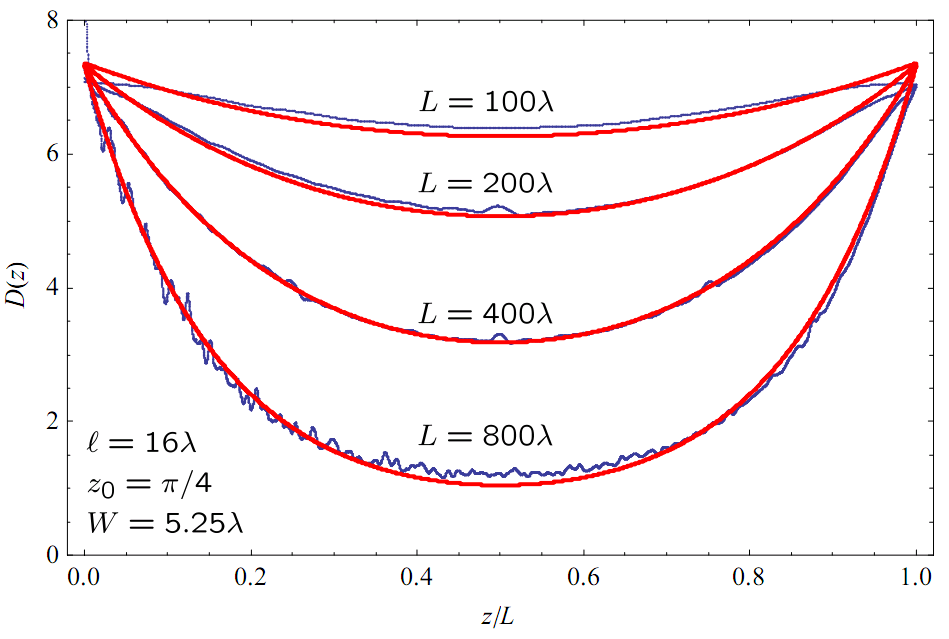
\includegraphics{pictures/Dz_passive}}}
\vskip -0.5cm
% NOTE: if a short caption is needed for figure list, use
%\caption[short desk]{long desk}
\caption[Position-dependent diffusion coefficient~$D(z)$ as predicted by self- consistent theory of localization (smooth red curves) and numeric results (rough blue lines) for quasi-1D waveguides with randomly-placed passive scattering potentials for varying system length~$L$, constant scatterer density, and width~$W$.]{Position-dependent diffusion coefficient $D(z)$ as predicted by self-consistent theory of localization (smooth red curves) and numeric results (rough blue lines) for quasi-1D waveguides with randomly-placed passive scattering potentials for varying system length~$L$, constant scatterer density, and width~$W$. Very good agreement for ballistic ($L=100 \lambda$), diffusive, and localized ($L=800 \lambda$) regimes. The term $\ell$ is transport mean free path, and $z_0$ is penetration depth.}
\label{fig:Dz_passive}
\end{figure}

%Method: How am I numerically modeling these criteria?}
To develop numerical models that can simulate wave transport in nonconservative media for individual realizations of disorder, this work implements the transfer matrix method~\cite{1981_MacKinnon_scaling,1992_Pendry,2003_Kettemann} 
% note: when MacKinnon cites tmm, he uses 1981_MacKinnon_scaling and 
% MacKinnon A 1994 J. Phys. Condensed Matter 6, 2511
for the entire waveguide. Essentially, the transfer matrix method matches boundary conditions before and after an event in a system where wave modes are quantized. Not only is the quasi-1D geometry experimentally viable~\cite{2009_Genack_PRB}, it also provides a convenient theoretical framework~\cite{1982_Dorokhov_DMPK,1988_Mello_Kumar_DMPK}. Here, waveguides described as ``quasi-1D'' have the following characteristics: (1)~quantized transverse modes due to boundary conditions, expressed as $E(y=0,W;\forall z)=0$ as for metallic edges, (2)~waveguide width $W$ less than $\ell_{tmfp}$ so that no significant transverse propagation occurs, and (3)~aspect ratio ($L:W$) is not fixed (i.e., $W$ is constant when $L$ is increased, with a fixed disorder density). Further, the propagation is confined to two dimensions in order to study a single polarization of electromagnetic radiation.

As shown in Appendix~\ref{sec:appendix_derivation_transfer_matrices_quasi1d}, the differential wave equation
\begin{equation}
\nabla^2 E(\vec{r}) = - \frac{\omega^2}{c^2} E(\vec{r})
\label{eq:wave_equation_electric_field_introduction}
\end{equation}
can be separated into perpendicular and parallel components (resolving wave vector $\vec{k}$ into $k_{\perp}$ and $k_{\parallel}$). Once the electric field solution is found, scattering potentials are introduced, initially as $\delta$ functions. The derivation of the transfer matrix method is \textit{ab initio} based on Maxwell's equations~\cite{1999_Jackson}, and no assumption about transport mean free path is made. 

For light waves, transverse wave quantization means that the modes of an electric field and its derivative can be written in the 
form of a vector. The translation of that field in vector form through a dielectric-filled space or past a scattering potential is described by a matrix, the rank of which is dependent on the number of transverse modes of the waveguide (c.f. Appendix~\ref{sec:appendix_derivation_transfer_matrices_quasi1d}). In 1D, the transfer matrix method takes the initial electric field $E_0$ and its derivative $E_0^{\prime}$ and translates to the field and its derivative over distance $\Delta x$:
\begin{equation}
 \left( \begin{array}{cc}
t_{11} & t_{12} \\
t_{21} & t_{22} \\
\end{array} \right)
\left( \begin{array}{c}
E_0 \\
E_0^{\prime}
\end{array} \right)
=
\left( \begin{array}{c}
E_{\Delta x} \\
E_{\Delta x}^{\prime}
\end{array} \right).
\end{equation}
Multiple scattering events are combined as $\hat{T}_{total} = \prod_i \hat{T}_i$. The product describes the effect of the medium on the transport of the incident light. Since the transfer matrices have finite rank, the scattering potentials used are actually a finite summation of Fourier components of the $\delta$ function. Although the purpose of the numerical model is a study of photonic transport in nonconservative media, the resulting electric field magnitude, plotted in Fig.~\ref{fig:electric_field_zoomed}, is a secondary benefit.

\begin{figure}
\vskip -0.5cm
\centerline{
\scalebox{.47}{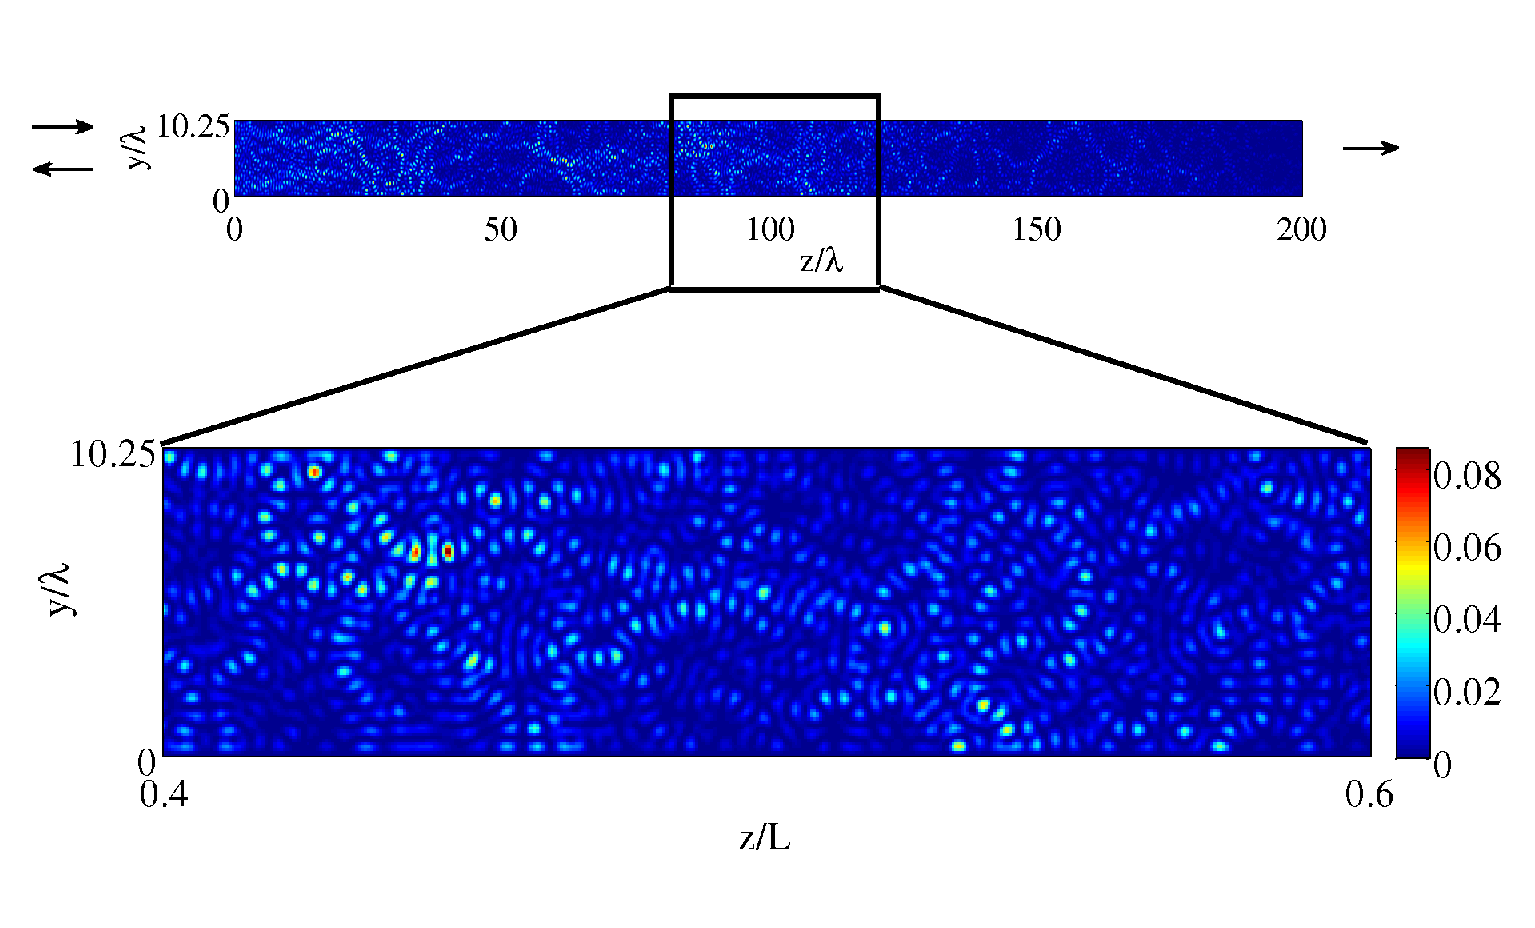
\includegraphics{pictures/electric_field_resonant_freq_zoom_normalized_z_box_arrows}}}
\vskip -0.5cm
% NOTE: if a short caption is needed for figure list, use
%\caption[short desk]{long desk}
\caption[Magnitude of electric field inside a quasi-1D waveguide for passive media in the diffusive regime.]{Magnitude of electric field inside a quasi-1D waveguide for passive media in the diffusive regime. Midsection of waveguide is shown (from $z/L=80/200$ to $z=120/200$) for a resonant frequency (higher than average transmission). Spatially varying field intensity (with continuous wave incident flux) demonstrates interesting microscopic behavior, even though the system is in the diffusive regime.
\label{fig:electric_field_zoomed}}
% The Poynting vector can plotted
% [don't say this because you aren't including a picture of the Poynting vectors.]
\end{figure}

The transfer matrix method is used in the field of transport~\cite{2007_Froufe-Perez_PRE}, but its application is usually limited either to RMT for perturbative study or directly only to the diffusive regime. These limitations are due to the fact that multiplication of numerical matrices results in inaccuracy due to divergent eigenvalues in the product~\cite{1968_Osedelec}.
% A simple showing of this would be nice
The numerical inaccuracy is detectable since each transfer matrix has determinant unity. % (due to conservation of flux?) 
The product of the matrices must retain a determinant of unity since 
%citation would be nice here, but most linear algebra books leave it as an exercise to the reader
%\begin{equation}
$\rm{det}(\hat{A})\rm{det}(\hat{B})=\rm{det}(\hat{A}\hat{B})$.
%\end{equation}
A self-embedding technique renormalizes the divergent eigenvalues and make this approach feasible~\cite{1999_yamilov_selfembed,1976_Bellman_Wing_embedding}.
%Although self-embedding technique applies to any numerical multiplication of many matrices, it is applied here to waveguides. %1D and planar quasi-1D waveguide geometries.
%In passive media, conservation of energy implies $T+R=1$ which is checked for validity of results.
The reliability of the transfer matrix method with self-embedding is demonstrated by comparing numerical simulation results of average unitless conductance $\langle g \rangle$ versus variance var$(g)$ to data yielded by a theoretical supersymmetry-based approach~\cite{2000_Mirlin}. With no fitting parameters, there is very good agreement (c.f. Fig.~\ref{fig:Mirlin_supersymmetry_g_varg}). Similarly, the diffusion coefficient from numerical simulation of passive media matches expected $D(z)$ (c.f. Fig.~\ref{fig:Dz_passive}).

\begin{figure}[t]
\vskip -0.5cm
\centerline{
\scalebox{.5}{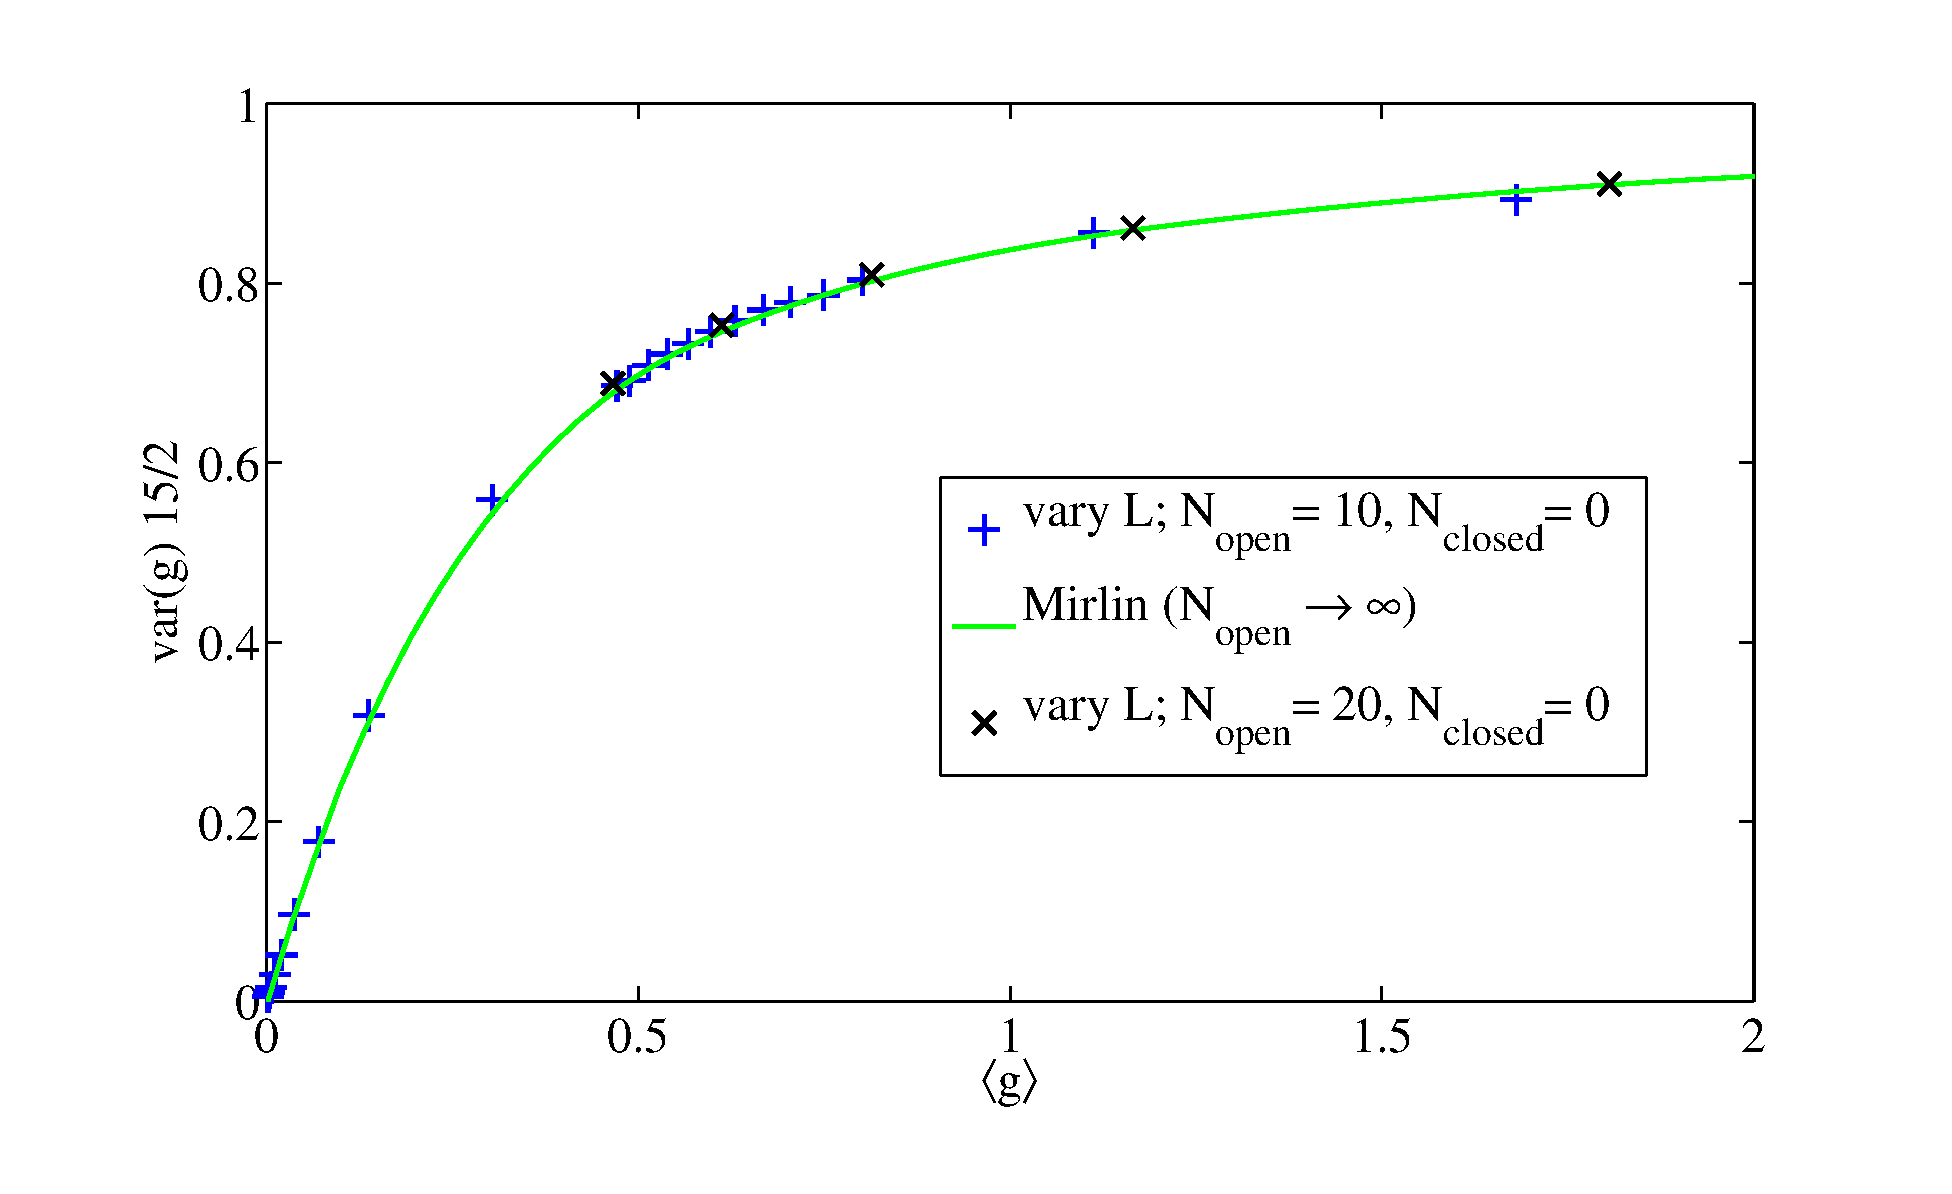
\includegraphics{pictures/var_g_versus_g_no_closed_channels}}}
\vskip -0.5cm
% NOTE: if a short caption is needed for figure list, use
%\caption[short desk]{long desk}
\caption[Theoretical prediction based on supersymmetric approach for average unitless conductance $g$ versus variance of $g$ for quasi-1D waveguide~\cite{2000_Mirlin} compared to results from numerical simulations described in Section~\ref{sec:method_numerical}.]
{Theoretical prediction based on supersymmetric approach for average unitless conductance $g$ versus variance of $g$ for quasi-1D waveguide~\cite{2000_Mirlin} compared to results from numerical simulations described in Section~\ref{sec:method_numerical}. No fitting parameters are used and good agreement is found. The $15/2$ accounts for the geometry of the waveguide. Many realizations of random media for each waveguide determined $\langle g \rangle$ and var$(g)$ for waveguides of two different widths (with the number of open channels $N_{open}$ determined by $W$) and varying system length $L$. The supersymmetry-based approach assumes the limit of an infinite number of propagating modes, but $N_{open}$ equal to 10 and 20 is sufficient.\label{fig:Mirlin_supersymmetry_g_varg}}
\end{figure}
  

\section{OUTLINE OF TRANSPORT REGIMES}
\label{sec:twod_plot}

To guide the study of the extension of the three passive regimes in nonconservative media, a two-parameter diagram (c.f.~Fig.~\ref{fig:regime_plot_main})  % Spring semester 2009, Ben and Dr Yamilov
enumerates types of transport behavior. The first parameter is system length $L$, which varies in relation to constant disorder density and waveguide width for passive media. The second parameter is gain or absorption strength. The two-parameter plot is needed to define specific signatures of diffusion and AL. The chapters that follow use the numerical model of waveguides to verify transitions between types of transport and to characterize behavior of LC such as the proposed $T/{\cal E}$ in nonconservative random media.

A single-valued parameter such as~$T/{\cal E}$ is useful even in this two-parameter space because it indicates only whether diffusion or AL descriptions apply to transport. However, not all single-valued LC are applicable for these systems due to the divergence of most observable parameters as RLT is approached with increased gain. Before determining which side of diffusion or AL is characterized by~$T/{\cal E}$, the behavior on both sides must be defined. Currently, no clear definitions of AL or diffusive behavior exist for nonconservative random media.

%\section{what is the plan?}
Figure~\ref{fig:regime_plot_main} describes types of transport in quasi-1D waveguides with random media; it has three passive regimes: ballistic (\textbf{B}), diffusive (\textbf{D}), localized (\textbf{L}) on the horizontal axis and gain (\textbf{G}) or absorption (\textbf{A}) strength on the vertical axis. The two-letter combinations on the plot denote a regime of specific behavior. The passive regime transitions (B/D/L) are characterized by the transport mean free path~$\ell_{tmfp}$ and localization length~$\xi$, as described in Section~\ref{sec:thesis_statement}. All lengths are normalized by wavelength~$\lambda$. 

\begin{figure}[t]
\vskip -.8cm 
% when scalebox=0.65, -2 gives the figure alone on page, -3cm give no margin at the top.
% when scalebox=0.65, -.8 is figure alone
% when scalebox=0.45, -2 gives not enough margin at top; -.5 and -.8 looks good
\centerline{
\scalebox{.65}{ % 0.65 would be largest
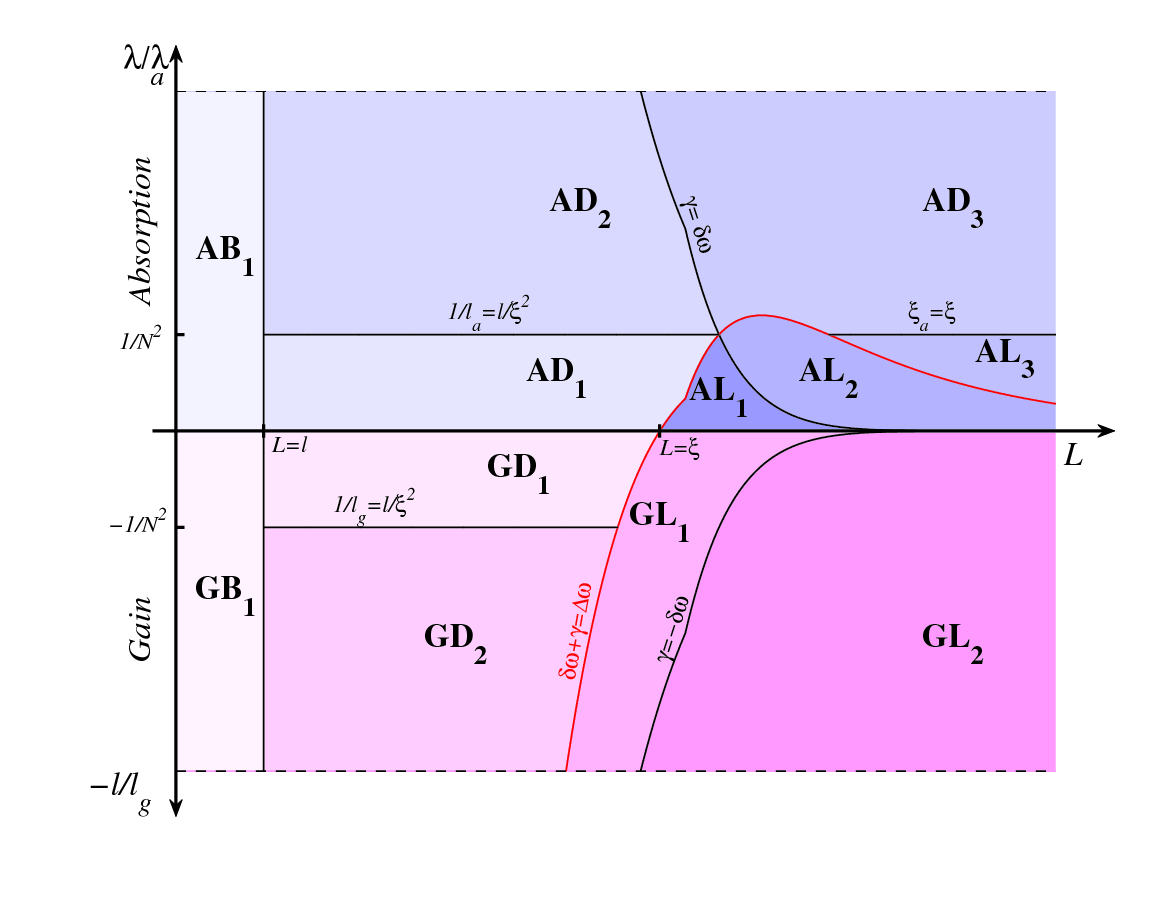
\includegraphics{pictures/regimes_plot_main}}}
\vskip -0.5cm
\caption[Various types of transport phenomena denoted by two-letter abbreviations (see text for explanation).]{Various types of transport phenomena denoted by two-letter abbreviations (see text for explanation). Each region is a permutation of the inequality of relevant characteristic lengths. Passive (conservative) transport regimes are on the horizontal axis, assuming constant disorder density and varying system length $L$. Plotted vertically, amounts of absorption or gain (nonconservative media) increase with distance away from the passive system horizontal axis. 
%Regime plot for quasi-1D random media. Lines denote transitions between regions of similar transport behavior; each region is denoted by a two-letter abbreviation. See text for explanation.
\label{fig:regime_plot_main}
}
\end{figure}

%It is important to note that characteristic lengths are defined in specific regimes. For example, 
%For brevity, only absorption is referred to, but the concepts apply equivalently to gain. 
The absorption (gain) rate $\gamma_{a,g}$ is the average number of absorption events per unit time, where an event refers to the particle removed (doubled) along a specific path. The absorption (gain) rate is the inverse of the absorption (gain) lifetime, 
%\begin{equation}
$\gamma_{a,g} = \frac{1}{\tau_{a,g}}$, 
%\end{equation}
where $\tau_{a,g}$ is the average propagation time of the particle before it is absorbed (doubled). The averaging is over many random particle paths. Given a characteristic time $\tau_{a,g}$, the characteristic absorption or gain length is 
%\begin{equation}
$\ell_{a,g} = \tau_{a,g} c$, 
%\end{equation}
where $c$ is the propagation speed of the particle. This characteristic length is the average distance prior to absorption (doubling) with respect to the path length. The $\ell_{a,g}$ is determined from the time-dependent diffusion equation in one dimension,
\begin{equation}
D \frac{\partial^2 I}{\partial z^2} = \frac{\partial I}{\partial t},
\label{eq:diffusion_equation_1D}
\end{equation}
to be 
% see /svn/bens/lab_notebook/20090422_dr_Yamilov_mtg_regime_change_for_plot.pdf
% equation 37
\begin{equation}
\ell_{a,g}= \left( \frac{d}{\pi^2}\right) \frac{L^2}{\ell_{tmfp}}.
\label{eq:ballistic_gain_abs}
\end{equation}
However, $\ell_{a,g}$ is already defined in the ballistic regime as the average length after which the particle is no longer present in a ballistic system due to absorption (doubled when gain is present). The system length $L$ (how far the particle would have gone along a ballistic path) should be replaced by a new diffusive-regime length, $\xi_{a,g}$. Eq.~\ref{eq:ballistic_gain_abs} can then be solved for $\xi_{a,g}$:
\begin{equation}
 \xi_{a,g} = \sqrt{\frac{\ell_{a,g} \ell_{tmfp}}{d}}.
\label{eq:diffusive_absorption_length}
\end{equation}
Physically, $\xi_{a,g}$ is the average length after which the particle is no longer present in a multiple-scattering system. To distinguish the two absorption (gain) lengths, $\xi_{a,g}$ is measured with respect to system length $L$ (rather than path length $L_D$), whereas $\ell_{a,g}$ is measured with respect to path length $L_D$. If $L$ is equal to $L_D$, then no diffusion is occurring and $\ell_{a,g}$ is equal to $\xi_{a,g}$. Usually, the literature does not distinguish between measurement of an absorption length with respect to diffusive path $L_D$ or measuring it with respect to system length $L$. There are two reasons for this ambiguity: first, experimentally, $L_D$ is harder to measure than $L$; second, the regime to which various lengths apply to is generally not specified.

For localized systems, it no longer makes sense to measure lengths with respect to path length since wave effects are dominant (i.e., ray optics do not apply). In this regime $\xi_{a,g}$ is used, but it is not defined in terms of $\ell_{a,g}$ as in Eq.~\ref{eq:diffusive_absorption_length}. The transition indicating whether or not absorption affects AL or not is set by $\xi_{a} = \xi$ (the horizontal line between $AD_3$ and $AL_3$ in Fig.~\ref{fig:regime_plot_main}). This transition in the diffusive regime is found by applying Eq.~\ref{eq:diffusive_absorption_length} to $\xi_{a,g} = \xi = N_{open} \ell_{tmfp}$ and solving 
\begin{equation}
N_{open}^2 \ell_{tmfp}^2 = \frac{\ell_{tmfp}\ell_{a,g}}{d}
\end{equation}
to get $\ell_{a,g} =d N_{open}^2 \ell_{tmfp}$. For the diffusive regime, this line indicates how much absorption (gain) is necessary to distinguish transport behavior from a passive system. The remaining curves in Fig.~\ref{fig:regime_plot_main} are derived from the density of state transitions, rather than the characteristic lengths.

For passive media, the width of peaks in transmission with respect to frequency ($\delta \omega$ of the Thouless criterion in Eq.~\ref{eq:Thouless_passive}) is inversely proportional to the escape lifetime (the average time until an input leaves the system). To account for absorption or gain, an additional term is needed~\cite{2005_Yamilov_correlations} in the form of a rate: 
%\begin{equation}
$\delta \omega +\gamma_{a,g}$.
%\end{equation}
Although the width of DOS $\Delta \omega$ also changes as a function of gain due to the Kramers-Kronig relation~\cite{1999_Jackson}, the perturbation can be disregarded since the amount of gain and absorption of interest is small. 
% boundaries
The Thouless criterion is adapted to nonconservative media by inclusion of the gain (sometimes referred to as negative absorption~\cite{1968_Letokhov}) or absorption rate $\gamma_{a,g}=\mp~c/\ell_{a,g}$:
\begin{equation}
\delta'=\frac{\delta \omega +\gamma_{a,g}}{\Delta \omega};
\label{eq:generalized_thouless}
\end{equation}
it is plotted as the red curve $\delta'=1$. Physically, this boundary signifies whether the width of quasi-modes or separation of spectral peaks is larger. An additional boundary introduced by inclusion of nonconservative media occurs when absorption or gain overcomes radiative leakage of an average quasi-mode of the system, as plotted by the black curve $\pm \gamma = \delta \omega$. %The remaining boundaries are straight lines and are determined by enumerating permutations of characteristic length scale inequalities. For example, in the diffusive regime, $L$, $\xi$, $\ell_{tmfp}$, and $\ell_{a,g}$ form a minimum basis for distinguishing transport behavior. 
%Enumerating all permutations of relevant length inequalities, a distinct set of transport behaviors has been found.
% caveat
Although each region is separated by a line in Fig.~\ref{fig:regime_plot_main}, the transition between regimes is actually continuous due to the use of many realizations of randomly placed scatterers. Given the boundaries between each region, two-letter abbreviations are defined for each unique transport behavior.

% transport behavior of each regime
In the ballistic regime $GB_1$, gain below ballistic lasing threshold is not expected to change transport behavior (and similarly for $AB_1$ when $\ell_a < L$). For a small amount of absorption or gain in regions $AD_1$ and $GD_1$, the diffusive transport is also expected to remain similar to passive media. The use of conditional statistics~\cite{2005_Yamilov_correlations} eliminates a small number of lasing media. With sufficient absorption, signatures of diffusion are reduced ($AD_2$) and suppressed ($AD_3$). In contrast, gain enhances fluctuations ($GL_1$) and leads to lasing ($GL_2$) on average for many realizations~\cite{1968_Letokhov}. Transport in region $GD_2$ is the equivalent of ``negative absorption'' in region $AD_2$. The remaining absorption regimes signify transition from distinct spectral peaks and leakage due to radiation ($AL_1$) to distinct spectral peaks with absorption dominating leakage ($AL_2$) to a continuous spectrum due to absorption with weak localization ($AL_3$).

% the hump of AL_2 is not separated because?

%The kink in the curves is the transition from diffusion based equations to Mirlin's projections~\cite{2000_Mirlin} in the localized regime.


% if I only have 10 minutes of the presentation, I will not have time for these regions
\begin{comment}
\begin{figure}
\vskip -0.5cm
\centerline{
\scalebox{.75}{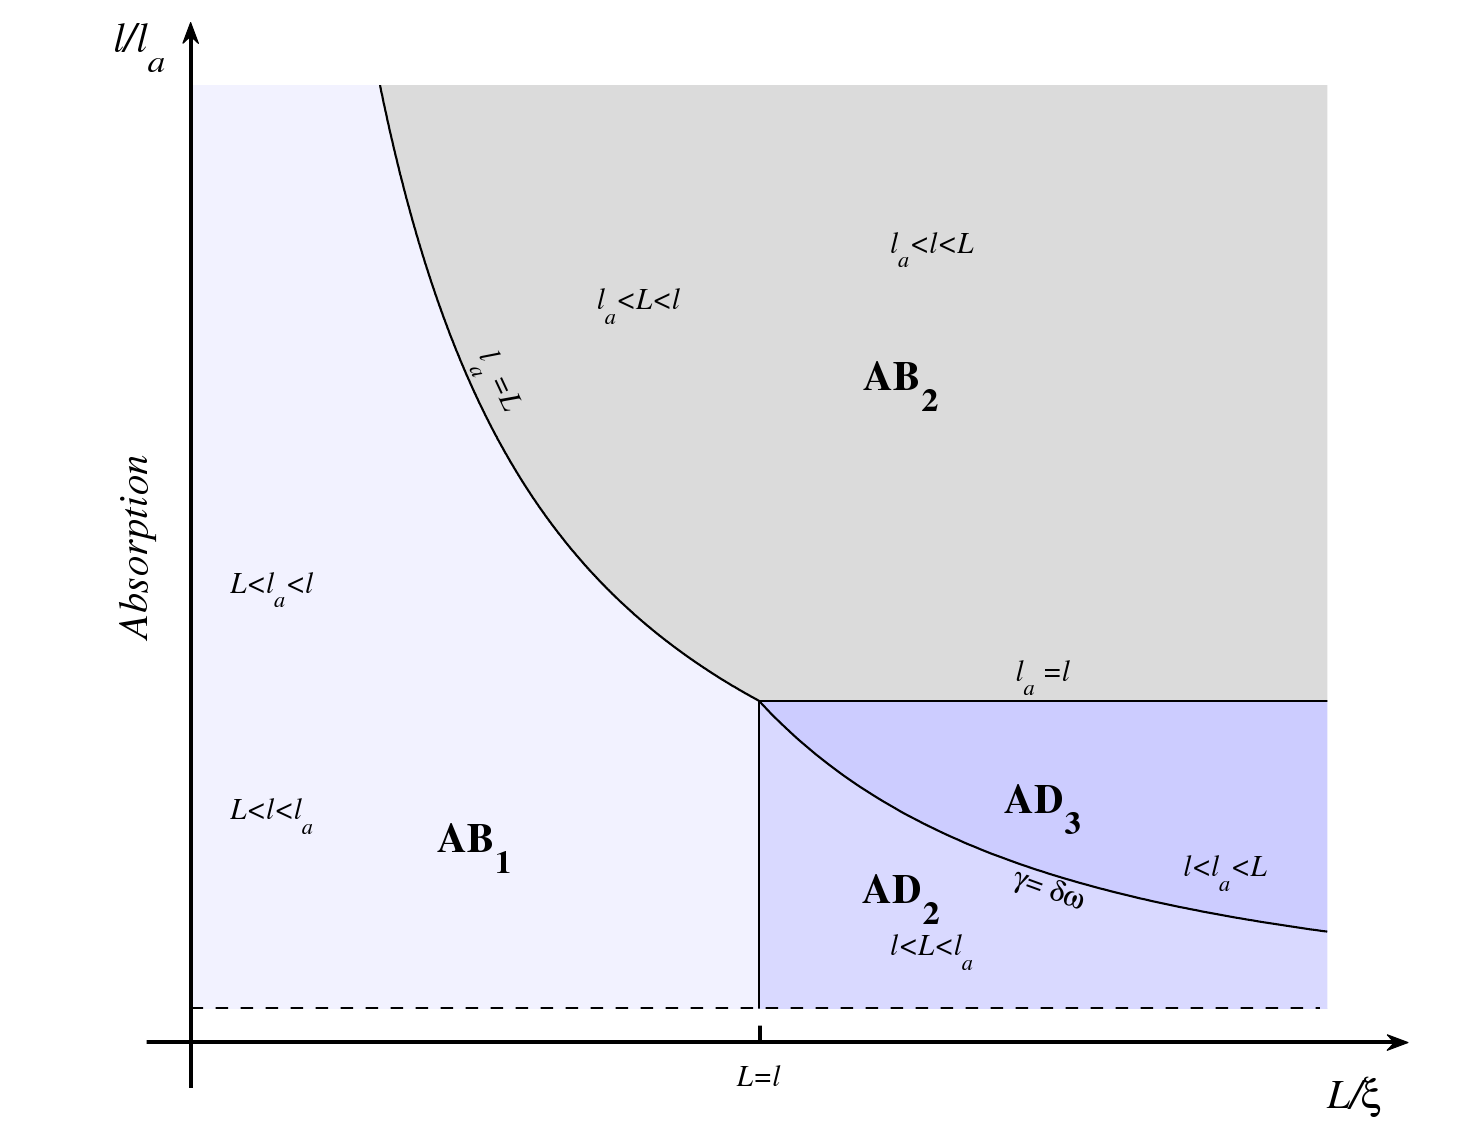
\includegraphics{pictures/regimes_plot_upper}}}
\vskip -0.5cm
%\caption[Upper regime plot (strong absorption) for quasi-1D random media.]{Upper regime plot (strong absorption) for quasi-1D random media. Each region is associated with an inequality of lengths. See text for explanation.}
\label{fig:regime_plot_upper}
\end{figure}

\begin{figure}
\vskip -0.5cm
\centerline{
\scalebox{.75}{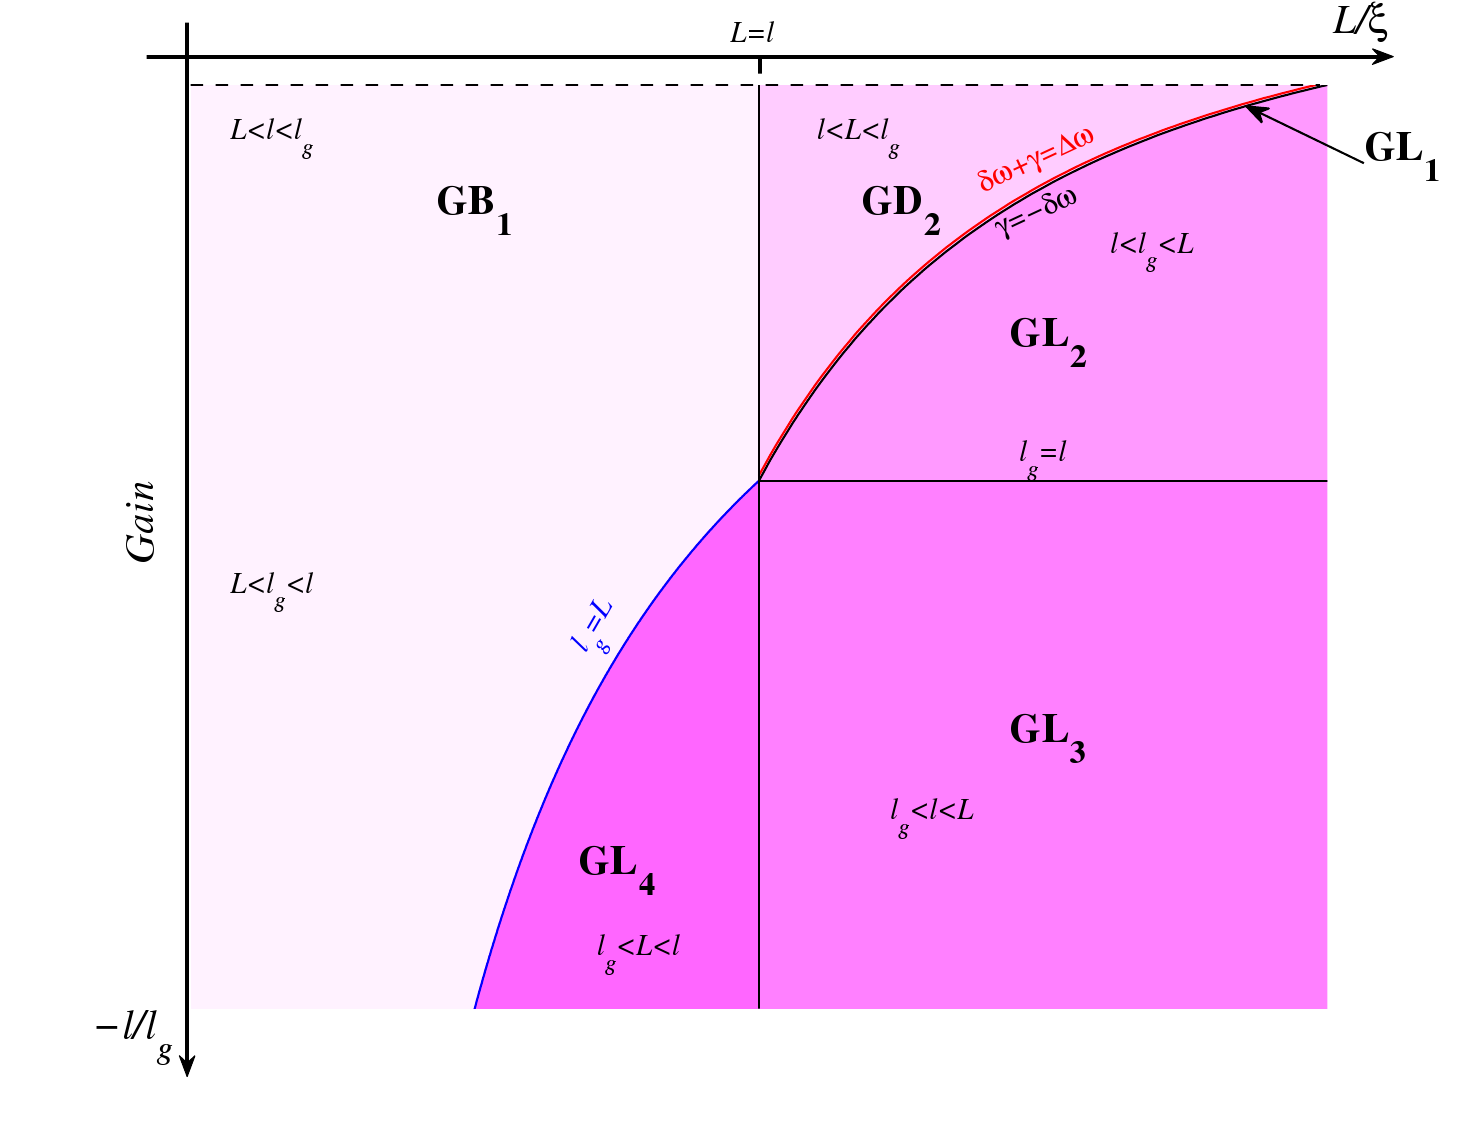
\includegraphics{pictures/regimes_plot_lower}}}
\vskip -0.5cm
%\caption{[Lower regime plot (strong gain) for quasi-1D random media.]Lower regime plot (strong gain) for quasi-1D random media. See text for explanation.}
\label{fig:regime_plot_lower}
\end{figure}
\end{comment}

% Note: analytical quasi-1D solution found by~\cite{1994_Beenakker_exact}

%I expect to be successful because I have sufficient tools (numerical model) and the plan is detailed and well-defined. Also, it is not too broad or too narrow.

To verify the boundaries and transport behaviors specified in Fig.~\ref{fig:regime_plot_main}, the numerical model for waveguides with random media is used to measure the criterion $T/{\cal E}$. In addition to determining the applicability of other LC such as $D(z)$, correlation functions, and the inverse participation ratio, this system makes possible the study of myriad other interesting topics. Examples include the effect of closed channels with gain~\cite{2010_Payne_closed}, wave front shaping~\cite{2008_Vellekoop_Mosk} to change transmission or focus field inside the medium, eigenmodes of transmission~\cite{1986_Imry}, and the visualization of Poynting vector field loops. The numerical model developed serves as a robust method for a comprehensive approach to investigating the transition from diffusion to AL for waveguides with nonconservative random media.

In this dissertation, each of the chapters are either published or in the process of submission to a peer-reviewed journal. Thus each chapter has an abstract, introduction, and conclusion. The first paper, Chapter~\ref{chap:TE_gain}, describes the applicability of the ratio of transmission to energy stored in a random media as a criterion for localization. Although both of these parameters diverge in the presence of optical gain, the ratio for each random medium does not. This criterion is developed in the context of a diffusive slab and also a numerical model of one dimensional layers of dielectric material. Since the lowest dimension for which the transition from diffusion to Anderson localization occurs in quasi-1D, there is a need for how to describe transport regimes with non-conservative media exists. The second paper, Chapter~\ref{chap:regimes}, details the development of boundaries between transport regimes in the two dimensional phase space for random media with gain and absorption. Another complication of the quasi-1D geometry is the inclusion of evanescent channels, which is studied in Chapter~\ref{chap:closed_channels}. We find that the effect of inclusion of evanescent channels is equivalent to renormalizing the transport mean free path. The last paper on random media in this dissertation, Chapter~\ref{chap:Dz_absorb}, demonstrates the validity of the position dependent diffusion coefficient $D(z)$ in the localized regime and in systems with absorption.

The remaining two chapters cover media with correlated disorder. Although random media exhibits unusual behavior, reproducibility is desirable for manufacturing. Thus algorithms specifying the non-random disorder (deterministic aperiodic systems) are of interest. The Thue-Morse pattern has a singular continuous Fourier spectrum, but this does not directly predict what transport properties are expected. In Chapter~\ref{chap:TM_to_TB} a mapping of the two dimensional Thue-Morse pattern is made to the tight-binding model. Then Chapter~\ref{eq:TM_physics} covers the anomalous transport properties, i.e.~coexistence of localized and extended states, exhibited by the Thue-Morse pattern.

% history
% current passive criteria
% mention self-embedding
%%20091214%%\section{one dimension}

\begin{comment}
 Outline:
1. T/${\cal E}$ as a criteria
  a. motivation
  b. why other criteria won't suffice
2. diffusive system
  a. solve diffusive equ analytically for slab with gain, 
       and we know diffusive system doesn't apply to localization
  b. find T, E. Plot a function of gain, L
  c. T/${\cal E}$ looks to be constant
  d. diffusion equation doesn't account for phase, which is the cause of localization
3. 1-D localization
  a. Setup: 1-D passive random system of alternating layers
  b. Results: peaks match/mismatch: T/${\cal E}$ is not smooth
  c. analysis: tunneling - look at analytical models
     i. double barrier potential 
     ii. periodic layers with single defect
  d. math analysis: energy is stored
  e. add gain
  f. closed system
  g. math reasoning, quantum well
  h. look for det[] = 0
  i. add gain
4. conclusion
5. future work

\end{comment}

%%%%%%%%%%%%%%%%%%%%%%%%%%%%%%%%%%%%%%%%%%%%%%%%%%%%%%%%%
\subsection {Motivation: T/${\cal E}$ as a parameter for localization with gain}
%%%%%%%%%%%%%%%%%%%%%%%%%%%%%%%%%%%%%%%%%%%%%%%%%%%%%%%%%

Localization criteria developed for passive systems may not be applicable for random media with gain. Transmission coefficients and the magnitude of their fluctuations diverge close to lasing threshold. In realistic systems, saturation prevents the divergence but introduces the dependence on saturation parameter. This may not carry the desired information about wave transport.

The Thouless criteria may not account for gain: % see NSF proposal, top of page 5,7
``The ensemble-averaged spectral correlation function might be dominated by the rare lasing configurations, thus the spectral correlation width could be equal to the lasing line width that depends on the properties of the gain material.'' [From NSF proposal.] [Need more background from NSF paper.] (Ioffe-Regel will not work in systems with gain?)

We confirm that transmission (T) and energy (${\cal E}$) both diverge as critical gain is approached in diffusive systems.  Either transmission~\cite{2000_chabanov_nature} or energy alone is not useful at critical gain, but perhaps a ratio of the two (T/${\cal E}$) will be non-divergent.

% what does the absorption model predict about resonant
% frequencies, standing waves, reciprocity?
% Perhaps we can extend our model to the absorption regime also?

%%%%%%%%%%%%%%%%%%%%%%%%%%%%%%%%%%%%%%%%%%%%%%%%%%%%%%%%%
\subsection {Diffusion: Slab geometry}
%%%%%%%%%%%%%%%%%%%%%%%%%%%%%%%%%%%%%%%%%%%%%%%%%%%%%%%%%

In starting to look for criteria for localization in systems with gain we first looked at diffusive systems. The reason for starting out in the diffusive model is because the diffusion equation can be solved analytically for the slab geometry, even when gain is added~\cite{1993_Lisyansky_diffusint}. We need to see how light is transmitted through media in general. 

We know there will not be any strong localization in systems described by the diffusion equation since the model does not keep track of phase.  Localization is based on interaction of waves and this interference is dependent on the phase.  Any model that does not account for phase or some derivative of phase will not be able to fully account for strong localization.

Gain cannot always be modelled by negative absorption. Close to lasing threshold the phase (i.e description of fields not intensities), fluctuations and the system dynamics become important. Far from lasing threshold, ``negative absorption'' is a reasonable way of introducing gain.
%Gain will be incorporated by adding an imaginary component to the dielectric constant.

Starting from the intensity distribution from Ref.~\cite{2004_Yamilov_intensity} we can find the transmission and reflection from Eq.~\ref{eq:diffusionequ}
\begin{equation}
J _{\pm} = \frac{c}{4} I \mp \frac{D}{2} \frac{dI}{dz}
\label{eq:diffusionequ}
\end{equation}
where $ J _- $ is the reflection flux, $ J _+ $ is the transmission flux, $I(z)$ is the intensity, and z is the position within the slab. Substituting the expression for $I(z)$ found in Ref.~\cite{diffusint}, we find
\begin{equation}
J _- (0) = \frac{c}{4} \frac{2 z _o q}{D} \\
\frac{\sinh(\alpha  (L-z _p)) + \alpha z_o \cosh(\alpha (L-z _p))}{\\
(1+ \alpha ^2 z_o ^2) \sinh(\alpha L) + 2 \alpha z_o \cosh(\alpha L)}
\label{eq:Jreflectionflux}
\end{equation}
and
\begin{equation}
J _+ (L) = \frac{c}{4} \frac{2 z _o q}{D} \\
\frac{\sinh(\alpha z_p) + \alpha z _o \cosh(\alpha z_p)}{(1+\alpha^2 z_o^2) \sinh(\alpha L) + 2 \alpha z_o \cosh(\alpha L)}
\label{eq:Jtransmissionflux}
\end{equation}
where $ J _{incident} = q $. We can also find the energy by integrating intensity over the entire system:
\begin{equation}
{\cal E} = \frac{q}{4 \pi D \alpha ^2} \left(1-\frac{\sinh(\alpha z_p) + \\
\sinh(\alpha (L-z_p))+\alpha z_o (\cosh(\alpha z_p) + \\
\cosh(\alpha (L - z_p))}{\sinh(\alpha L (1+\alpha^2 z_o^2))+\\
\cosh(\alpha L 2 \alpha z_o)}\right)
\label{fig:Jenergy}
\end{equation}
We plot transmission, Eq.~\ref{eq:Jtransmissionflux},and reflection, Eq.~\ref{eq:Jreflectionflux}, with and without normalization by energy ${\cal E}$, Eq.~\ref{fig:Jenergy}, as functions of gain and absorption in Fig.~\ref{fig:diffusiveRTRETE}.  
\begin{figure}
\vskip -0.5cm
\centerline{
\scalebox{0.4}{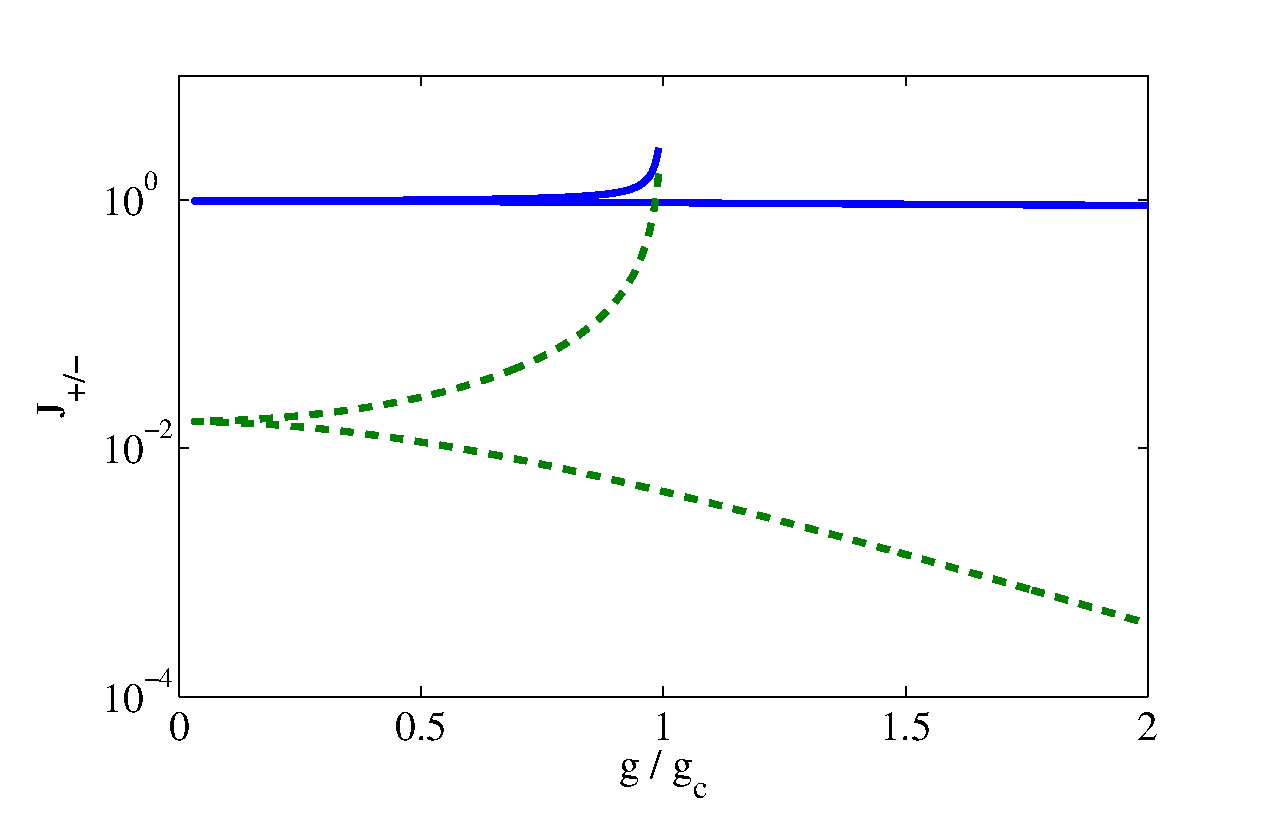
\includegraphics{pictures/yamilov_fixed_L_variable_gain_R_T}}
\scalebox{0.4}{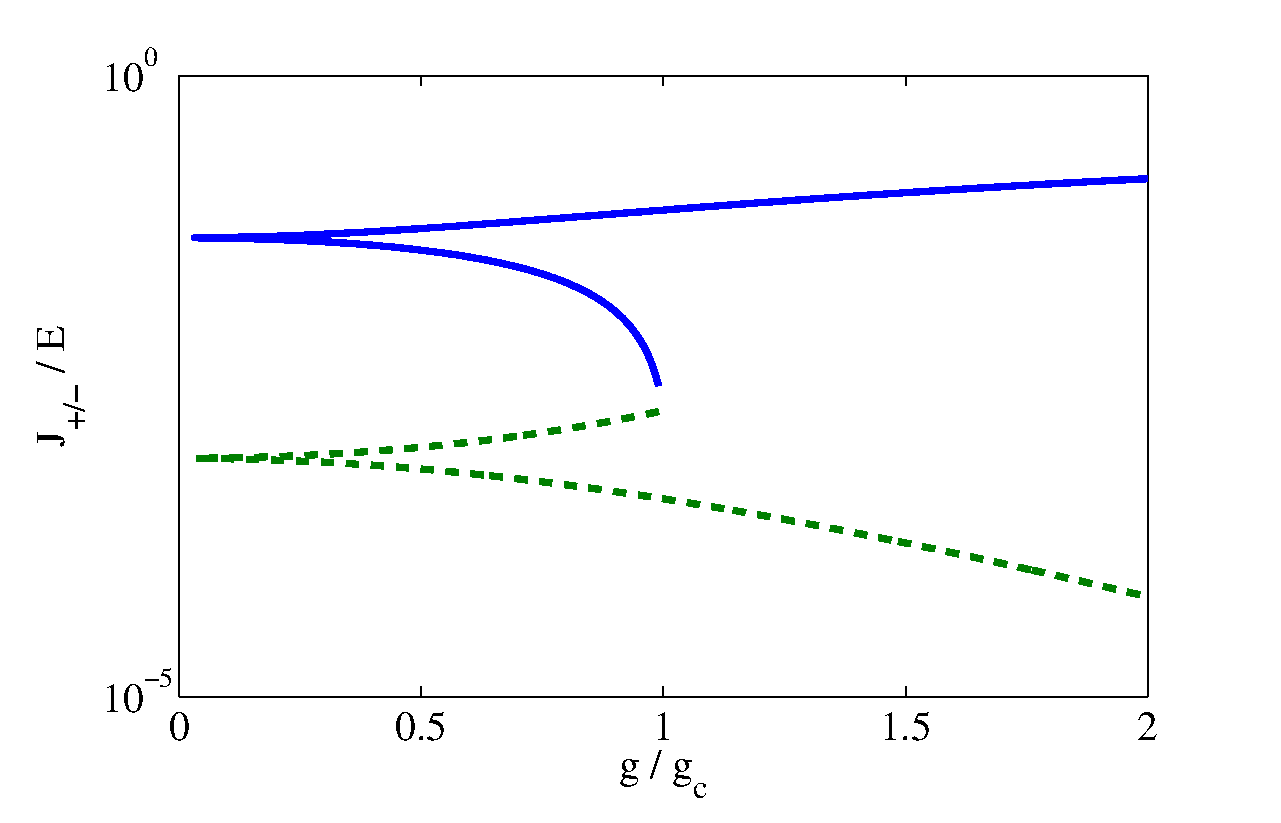
\includegraphics{pictures/yamilov_fixed_L_variable_gain_R_T_divided_by_Energy}}
}
\vskip -0.5cm
\caption[Transmission and reflection are plotted for increasing gain and absorption coefficients.]{Transmission and reflection are plotted for increasing gain and absorption coefficients. In the left plot dotted green line is transmission and solid line blue is reflection. In the left plot the upper dotted green and upper solid blue lines are transmission and reflection with increasing amounts of gain, both diverging at the critical gain value. The lower dotted green and lower solid blue lines are absorption.  In the right plot we see transmission/energy and reflection/energy.  Now when gain is added neither T/${\cal E}$ (upper dotted green line) nor R/${\cal E}$ (lower solid blue line) diverge at critical gain, and they both reach the same value. T/${\cal E}$ (lower dotted green line) and R/${\cal E}$ (upper solid blue line) in the absorption regime do nothing unexpected.}
\label{fig:diffusiveRTRETE}
\end{figure}

As critical gain is reached both transmission and reflection diverge asymptotically in Fig.~\ref{fig:diffusiveRTRETE} a according to
\begin{equation}
q \frac{z_o + z_p}{\pi} \frac{\alpha _c ^2}{\alpha _c - \alpha}
\end{equation}

Plotting the ratios of reflection to energy $( \frac{J_-}{\cal E} ) $
and transmission to energy $( \frac{J_+}{\cal E} ) $ in Fig.~\ref{fig:diffusiveRTRETE}
we see two things: T/${\cal E}$ does not diverge at critical gain, and the ratios 
of R/${\cal E}$ and T/${\cal E}$ match
at the critical gain. This tells us that T/${\cal E}$ may be a good
criteria for detecting localization (whereas both T and
R are divergant at critical gain).  Note that although
R/${\cal E}$ doesn't diverge, we don't use it because transmission may be 
easier to measure.

Another method for reaching a lasing state is to have a certain
amount of gain for a material and then adjust the length of the
sample until a critical length is reached such that the leakage
(this is an open system) is compensated by the cumulative
effect of the gain in the material. We see similar behavior
for the reflection and transmission (divergence of both transmission
and reflection in systems
near the critical length) versus R/${\cal E}$ and T/${\cal E}$ ratios (both converge
to same value at critical gain, both are non-divergent) in this
alternate analytical diffusion model.

The last thing we investigate in the diffusive system
is how the distribution of the intensity in the sample changes
for active systems and systems with absorption. When gain
is added there is more energy stored in the sample, as compared
to the passive and absorption regimes. See
Fig.~\ref{fig:diffusiveIntensityDistribution}. We also see that the intensity
decreases as it passes through the sample. If light were
shined on the other side of the sample we would see the decay
in intensity flip (decreasing from a maxium at x=L to near
zero at x=0).

\begin{figure}
\vskip -0.5cm
\centerline{\scalebox{0.4}{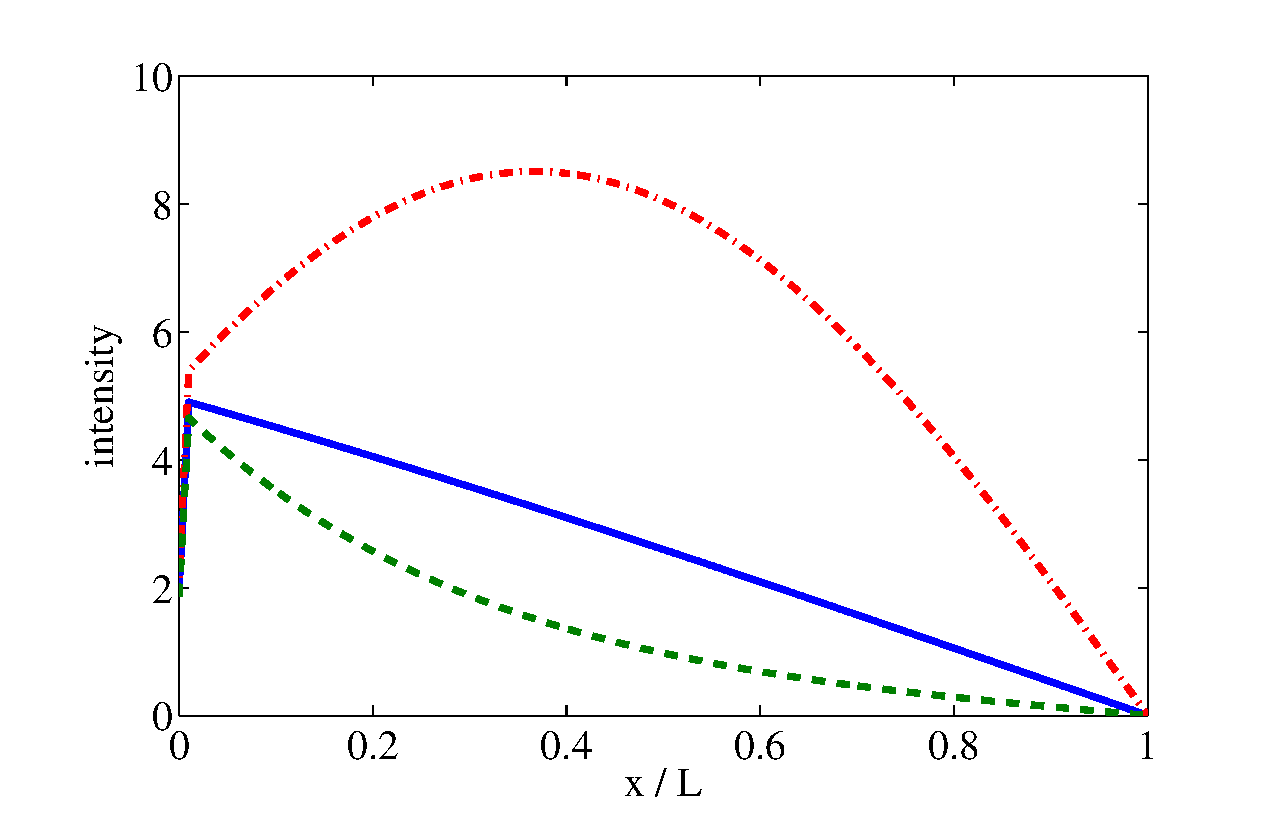
\includegraphics{pictures/yamilov_diffusive_intensity_distribution}}}
\vskip -0.5cm
\caption[Intensity distribution for the diffusive system.]{Intensity distribution for the diffusive system. Top red dotted line is 
the sample with gain, middle solid blue line is passive sample, lower dotted green line
is sample in the absorption regime. We can see that the amount of gain or absorption in the sample affects the field in the sample. This is verified in non-diffusive models.}
\label{fig:diffusiveIntensityDistribution}
\end{figure}

%%%%%%%%%%%%%%%%%%%%%%%%%%%%%%%%%%%%%%%%%%%%%%%%%%%%%%%%%
\subsection {Localization: stacks of dielectric layers model}
%%%%%%%%%%%%%%%%%%%%%%%%%%%%%%%%%%%%%%%%%%%%%%%%%%%%%%%%%

\subsubsection{Description of Setup}

We consider a passive system having layers of alternating ($\epsilon = 1$ and $1.2$) dielectric material, resulting in alternating refractive index ($n = \sqrt{\epsilon}$). This pair of layers is repeated to create 1000 pairs. One last $\epsilon = 1$ layer is added to the end to create a symmetric stack of 2001 layers. Then the total sample has length L. Randomness is introduced by varying the width of each $\epsilon=1.2$ layer. The variance of the random layers is such that localization length is between L/2 and L/5. Gain or absorption can be arbitrarily added by changing the value of the dielectric to be complex or negative, respectively, (but not both). Fig.~\ref{fig:dimaSetup} schematically shows the setup. These parameters put the model in the localization regime ($a\ll\lambda\ll L$). [What is a?] Where $\lambda$=wavelength, L is system length. The frequency range is chosen so that single parameter scaling is satisfied. [citation?]

\begin{figure}
\vskip -0.5cm
\centerline{\scalebox{0.8}{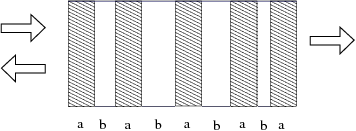
\includegraphics{pictures/dima_setup_cartoon}}}
\vskip -0.5cm
\caption[Layer setup for alternating pairs of dielectric.]{Layer setup for alternating pairs of dielectric. %``A'' and ``B'' form a pair.  
Solid blue layer A has a constant width, while the width of B has uniformly random variance of width between 1.1 and .9.  Light is incident on the left side of the sample with amplitude 1. Some light is reflected to the left and some is transmitted to the right.}
\label{fig:dimaSetup}
\end{figure}

Light is shone on one side of the material (from left to right) and the propagation of the light through the sample is calculated using Maxwell's equations and the transfer matrix method. The transfer matrix method is covered in detail around page 44 in a text book by Mello and Kumar\cite{2004_Mello_Kumar_book}. See also Appendix A.
% starting at equation 2.165
% see also notes 20080127
As a check, the magnitude of transmission and reflection add to one is verified.

% too technical
\begin{comment}
We multiply 2x2 matrices together (for 2001 layers). However, because of rounding error (using fortran 90) we need to use self-embedding technique~\cite{1999_yamilov_selfembed}. This means doing 200 matrix multiplications (resulting in a single 2x2 matrix) and then multiplying that by the next 200 matrices. Repeat for a total of five chunks. No re-normalization of the 2x2 matrices is necessary.

The amount of numerical data of this one-dimensional system scales with the number of layers (2001). Usually one considers many frequencies and/or many realizations. The results give managable dataset sizes (on the order of Megabytes) and the computational time is on the order of minutes.
\end{comment}

Using the computational model the cumulative energy in the system and the transmission are found for a given frequency. Then we scan many frequencies. Then in order to get generalized behavior we alter the random widths to produce another sample. Repeat to find ensemble behavior. 

We chose not to take any averages; rather we look at a single realization of disorder and attempt to understand it. Once the behavior is understood for a single instance we can develop a general phenomenological explaination.

\begin{figure}
\vskip -0.5cm
\centerline{\scalebox{0.5}{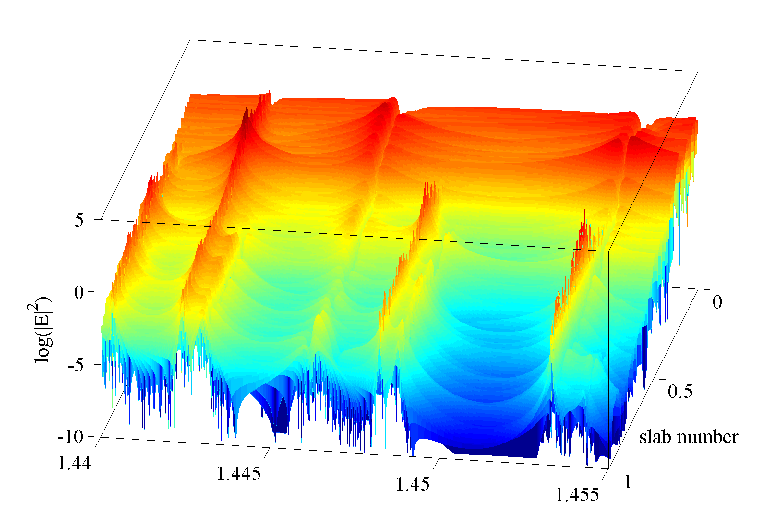
\includegraphics{pictures/electric_field_in_sample}}}
\vskip -0.5cm
\caption[The log of electric field in a random sample for a range of frequencies versus position in the sample.]{The log of electric field in a random sample for a range of frequencies versus position in the sample. Without localization pure exponential decay is expected. This can be seen between $\omega$ =  1.45 and 1.453 as a straight line descending from the incident side at x/L=0 down to a minimum at x/L=1. Everywhere else in the sample localization effects are observed. At $\omega$ = 1.4425 a peak higher than the incident value can be seen. This would correspond to Fig. \ref{fig:onequarterthreequarterelecfield}a. At $\omega$ = 1.4475 there is an intial linear decline, then a peak, then further linear decline  (exponential decay), similar to Fig.~\ref{fig:onequarterthreequarterelecfield}b. A 2-D version of this plot can be seen in~\cite{2006_Genack_1d}.}
\label{fig:electricFieldInSample}
\end{figure}

This computational configuration has been realized experimentally with one dimensional experiments using microwaves by Genack~\cite{2006_Genack_1d}, Luna-Acosta~\cite{2008_LunaAcosta} and John Scales~\cite{2006_Scales}. Fig.~\ref{fig:electricFieldInSample} is the electric field plotted on a log scale for many frequencies. The electric field is related to the energy distribution in the sample.  [Explain importance, compare to Genack Nov 07 paper]

%%%%%%%%%%%%%%%%%%%%%%%%%%%%%%%%%%%%%%%%%%%%%%%%%%%%%%%%%
\subsubsection {Results for Passive Random Layers Model}
%%%%%%%%%%%%%%%%%%%%%%%%%%%%%%%%%%%%%%%%%%%%%%%%%%%%%%%%%

From the computational model we see peaks in transmission do not always have the corresponding peaks in energy (Fig.~\ref{fig:tenkenergytransmission}). We will call the frequencies for which transmission peaks occur resonant frequencies. From this plot of transmission and energy versus frequency we can tell that the ratio T/${\cal E}$ is not going to be flat since there are spikes in transmission that do not have the counterpart in energy.

\begin{figure}
\vskip -0.5cm
\centerline{\scalebox{0.5}{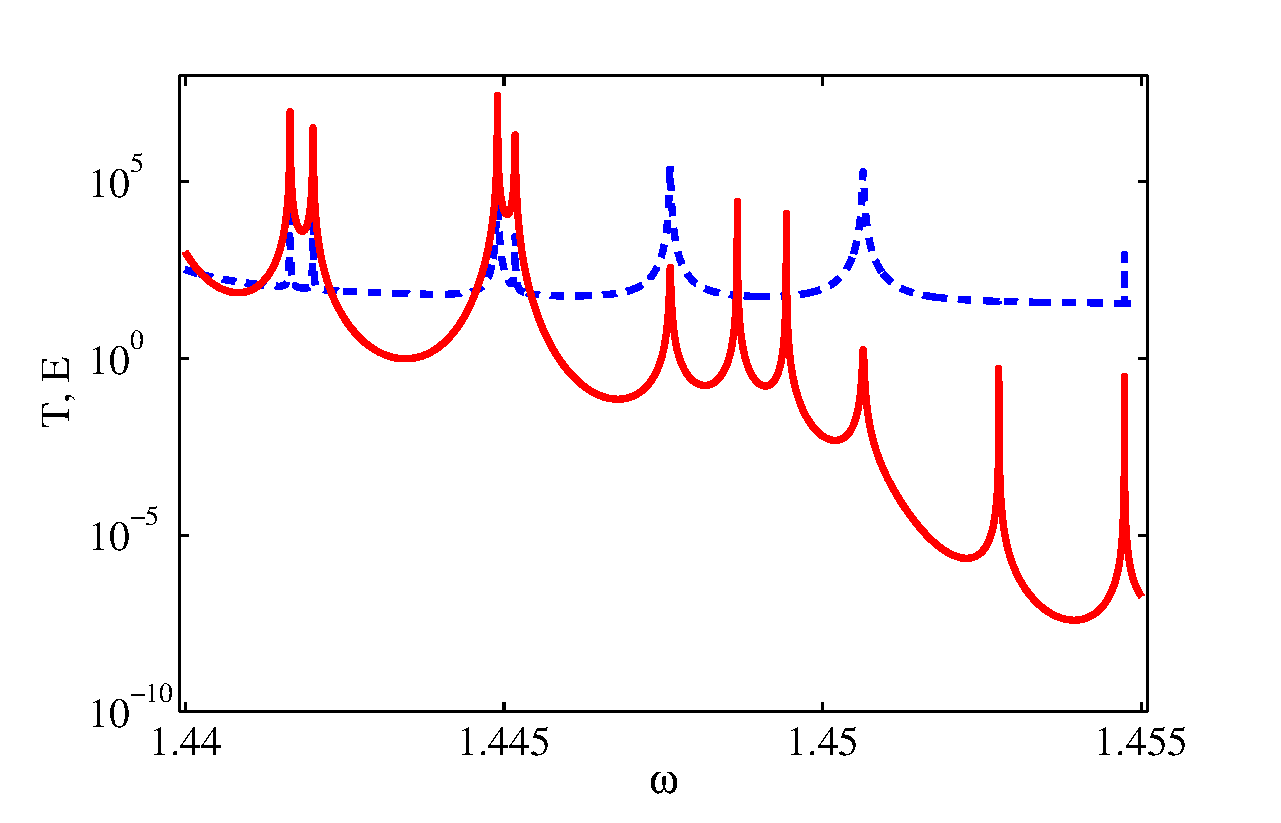
\includegraphics{pictures/tenk_energy_transmission_v_freq}}}
\vskip -0.5cm
\caption[Transmission as a function of frequency (omega) is compared to the total energy in the sample.]{Transmission as a function of frequency (omega) is compared to the total energy in the sample. This single represenative realization demonstrates that T/${\cal E}$ in the passive system will not be smooth. Transmission and energy sometimes share peaks for certain frequencies, but some peaks in transmission have no decernable peak in energy (even on a log plot with no noise).
%for left-to-right illumination.
}
\label{fig:tenkenergytransmission}
\end{figure}

% SIDE NOTE on A and B
Another quantity we can calculate in our computational model (in addition to the electric field and its derivative) is the amplitudes of the left and right traveling waves: A and B. Electric field in each layer is
\begin{equation}
\begin{gathered}
{\cal E}(x) = A \exp(i k n x) + B \exp(-i k n x) \\
A = \frac{1}{2} (E - i \frac{1}{k} \frac{dxi}{dx}) \\
B = \frac{1}{2} (E + i \frac{1}{k} \frac{dE}{dx})
\end{gathered}
\end{equation}
For resonant frequencies $ \| A \| \simeq \| B \| $ , which implies that it is almost like a standing wave with very little energy leakage, which is expected.

%                      For off resonant frequencies...(I don't have a plot of the A and B.)
% END SIDE NOTE

If the light is incident on the same sample but from the other side (ie right-to-left orientation) we see a different plot for transmission and energy versus frequency. Again, some peaks in transmission have no corresponding peak in energy while others do.

[Need a T, ${\cal E}$ v. freq plot showing RL is different]

Fluctuating T/${\cal E}$ is not of a significant concern, since we are in the passive system but the fact that it depends on illumination (from left of from right) is. % need to explain this concern more
It means that if we use this as a criterion, we will get a different value depending on how we perform the measurement. We will pay attention to this fact when we introduce the gain.

We investigate what is going on at those peak transmission frequencies. We would like to know why some peaks in transmission have corresponding peaks in energy while others do not. We also notice there are no cases where a peak in energy occurs and not transmission.

First, we confirm that for off-resonant frequencies we see exponential decay of the electric field through the sample. This is expected for random media in localization regime. When the exponential decay is plotted on a log scale we get a straight line.

Now we pick one resonant frequency and plot the electric field in the system. This is equivalent to looking at the energy inside the system. 
\begin{figure}
\vskip -0.5cm
\centerline{
\scalebox{0.4}{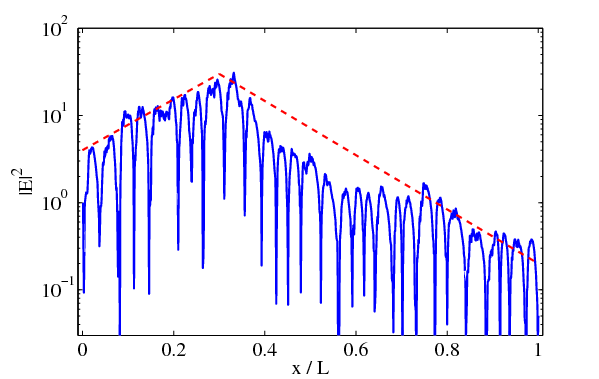
\includegraphics{pictures/rlz1_elecfield_14}}
\scalebox{0.4}{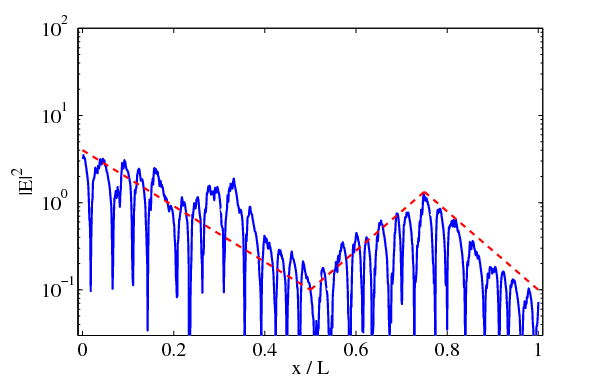
\includegraphics{pictures/rlz1_elecfield_34}}}
\vskip -0.5cm
\caption[In the left plot of the electric field (which is proportional to the energy stored in the sample) in the random media at resonant frequencies on a log scale there is a maximum near $ \frac{L}{4}$.]{In the left plot of the electric field (which is proportional to the energy stored in the sample) in the random media at resonant frequencies on a log scale there is a maximum near $ \frac{L}{4}$. This means there was exponential growth to the  center of localization, followed by exponential decay. The ratio of the amplitude at x=0 to x=L is approximately equal to the transmission. In the right plot we see a peak in electric field (energy) at $ \frac{3L}{4} $. For light to reach the center of localization  the light first exponentially decays, then grows, and falls again. The red dotted lines are the estimated slopes, which correspond to $\exp(\pm x/\xi)$.} 
\label{fig:onequarterthreequarterelecfield}
\end{figure}

Based on our analysis of many peaks in transmission, we conclude:
(i) At the frequencies where peaks in transmission 
and energy occur together there is a center of localization at $ 0 < x < \frac{L}{2}$. 
(ii) Where there is no corresponding peak in energy 
for a peak in transmission the center of localization occurs $ \frac{L}{2}<x<L $. 
We will use examples where the center of localization
happens at $ \frac{1}{4} $L, $ \frac{1}{2} $L, 
and $ \frac{3}{4} $L as canonical centers of localization
and we will treat them as specific examples.  Other 
positions can be interpolated.

We would like to know why the energy distributions 
change when the position of the center of localization changes.
The linear (when viewed on a semilogy scale) slopes
in these plots correspond to the localization length.
This behavior has been considered by Azbel, but only for $ 0 < x < \frac{1}{2} $L.~\cite{1983_Azbel_zeroTemp}

We calculate the energy stored in the system for 
different positions of a single center of localization
and plot Eq.~\ref{eq:energyposition} in 	% need to say how we got this equation?
Fig.~\ref{fig:peaksmatchnotmatch}, which explains
different ratios of the energy peak to the peak transmission.

\begin{equation}
{\cal E}(x) = \left\{
\begin{array}{l l}
%  \xi (-1 + 2\exp( \frac{x_1}{\xi} ) -  \exp( \frac{2 x_1-L}{\xi} )       \\ %& \quad \mbox{if x < \frac{1}{2}L}\\
%  \xi ( 1 + 2\exp( \frac{2 L-3 x_2}{\xi} ) - 3\exp( \frac{-2 x_2-L}{\xi} )  %& \quad \mbox{if x > \frac{1}{2}L}
  \xi (-1 + 2\exp( \frac{x_1}{\xi} ) -  \exp( \frac{2 x_1-L}{\xi} )      &  \quad \quad  if \quad x < \frac{1}{2}L  \\
  \xi ( 1 + 2\exp( \frac{2 L-3 x_2}{\xi} ) - 3\exp( \frac{-2 x_2-L}{\xi} )  & \quad \quad if \quad x > \frac{1}{2}L
\end{array} \right.
\label{eq:energyposition}
\end{equation}

%%%%%%%%%%%%%%%%%%%%%%%%%%%%%%%%%%%%%%%%%%%%%%%%%%%%%%%%%
\subsubsection {Passive Non-random 1D Models}
%%%%%%%%%%%%%%%%%%%%%%%%%%%%%%%%%%%%%%%%%%%%%%%%%%%%%%%%%

Normally when an electromagnetic wave is incident on a
material that does not allow transmission the wave
exponentially decays in the material.

Any wave that does make it through the material can be
said to have tunneled through the material.  Tunneling phenomenon
is present in quantum mechanics and band gap materials.
We analyze two idealized passive analytical models to confirm 
the behavior observed in the previous section. 

The first system consists of a potential barrier 
and the energy of incident wave is smaller then height of the barrier.
To introduce what would be a center of localization in
a random system we add a small well in the barrier (making
two close potential barriers).
The second model is a periodic structure with a single
defect acting as the analog of the center of localization.
The advantage of these analytical models is that we can
manually position what would be the center of localization
by specifying where the well is and where the defect
is, respectively. This is in comparison to the random model,
where we can not specify where the center of localization should be.

On a linear scale the behavior of the wave magnitude 
in the double barrier potential model is not
obvious, but when the same wave is plotted on a log
scale (Fig.~\ref{fig:barrierdefectlog}) it is
easy to see the comparison to the
random model.  Straight lines of increasing and
decreasing wave amplitude for a and c are the same as the canonical
wave forms in Fig.~\ref{fig:peaksmatchnotmatch} a and b.

\begin{figure}
\vskip -0.5cm
\centerline{
\scalebox{0.3}{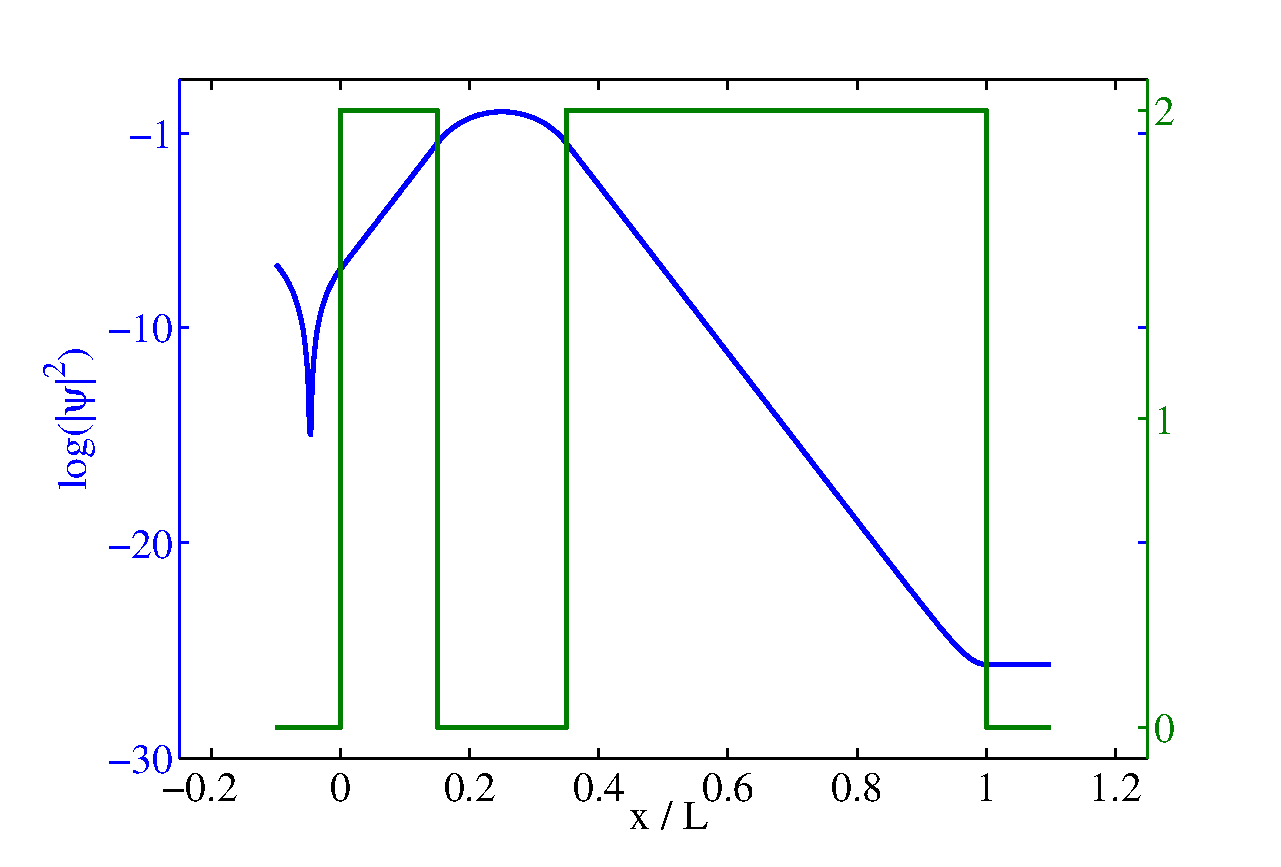
\includegraphics{pictures/barrier_defect_at_14_waveform_log}}
\scalebox{0.3}{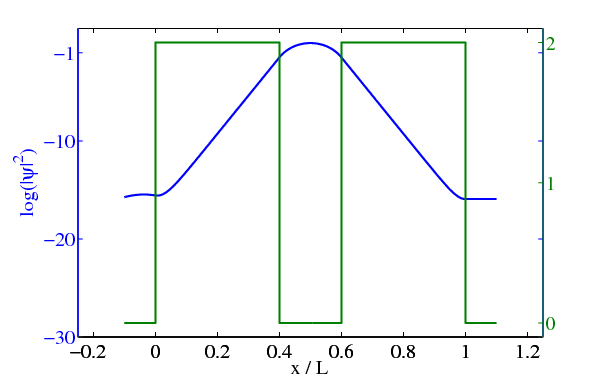
\includegraphics{pictures/barrier_defect_at_12_waveform_log}}
\scalebox{0.3}{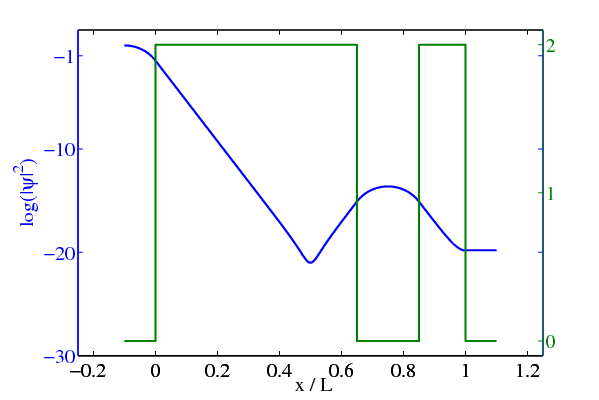
\includegraphics{pictures/barrier_defect_at_34_waveform_log}}}
\vskip -0.5cm
\caption[A wave incident from the left (solid blue line) on a potential barrier with potential well (dotted green) on semilogy scale looks  very similar to the electric field (aka energy) in the random system (Fig.~\ref{fig:peaksmatchnotmatch}).]{A wave incident from the left (solid blue line) on a potential barrier with potential well (dotted green) on semilogy scale looks  very similar to the electric field (aka energy) in the random system (Fig.~\ref{fig:peaksmatchnotmatch}).
We hypothosize that tunneling may be the reason for the
exponential decay and growth. Also seen in 
\cite{2004_Bliokh_wavelet}, but this is cleaner.}
\label{fig:barrierdefectlog}
\end{figure}

In the periodic layers with single defect the plots are the similar to the potential barrier model results, but with a more pronounced peak. For this analytical model we manually position the defect (instead of the potential well).

\begin{comment}
\begin{figure}
\vskip -0.5cm
\centerline{
\scalebox{0.3}{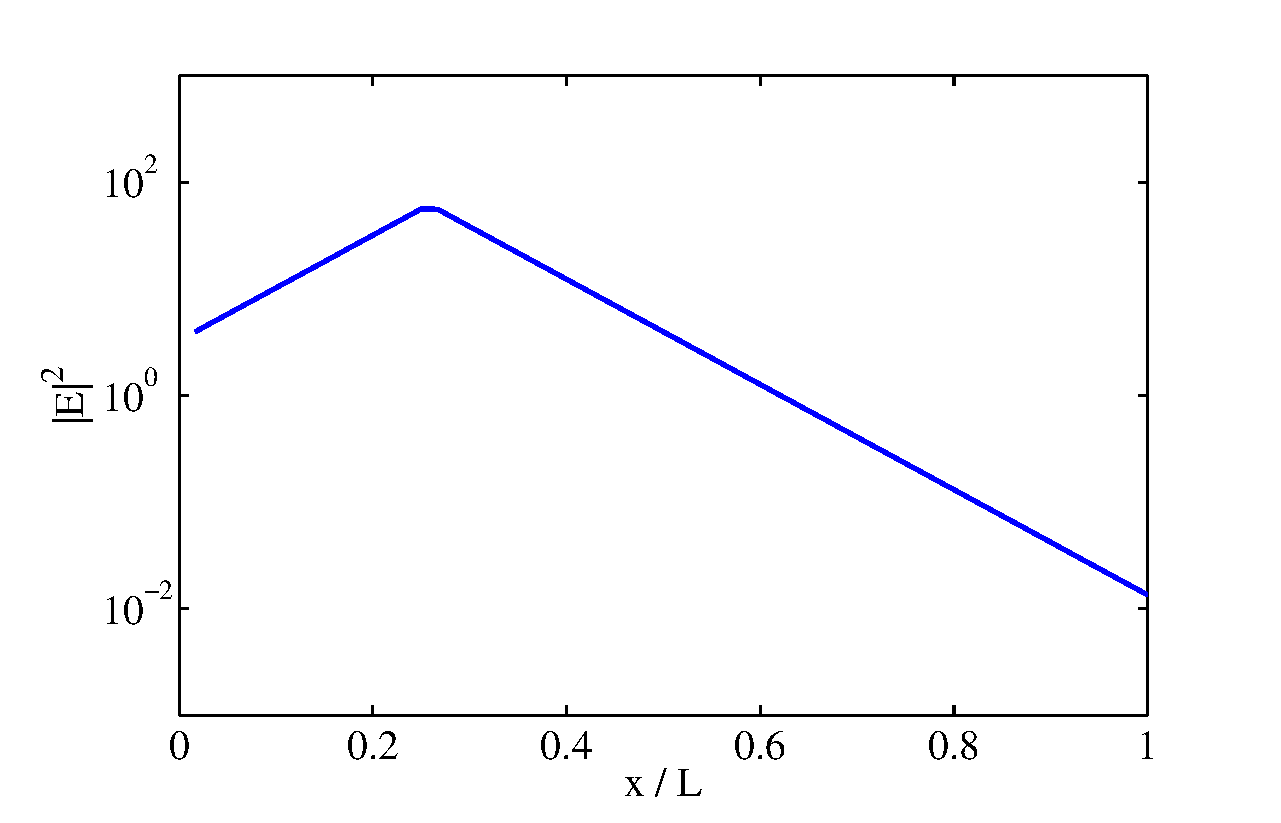
\includegraphics{pictures/passive_defect_14}}
\scalebox{0.3}{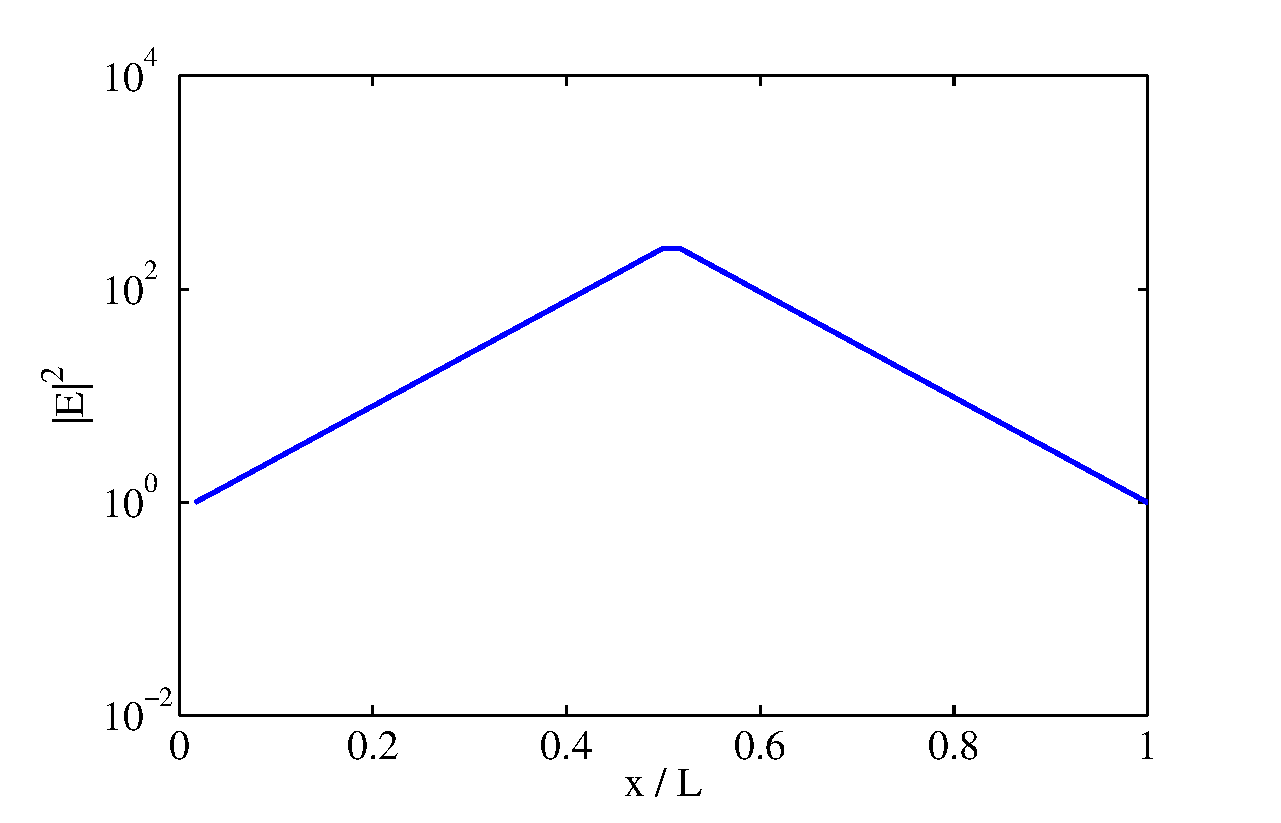
\includegraphics{pictures/passive_defect_12}}
\scalebox{0.3}{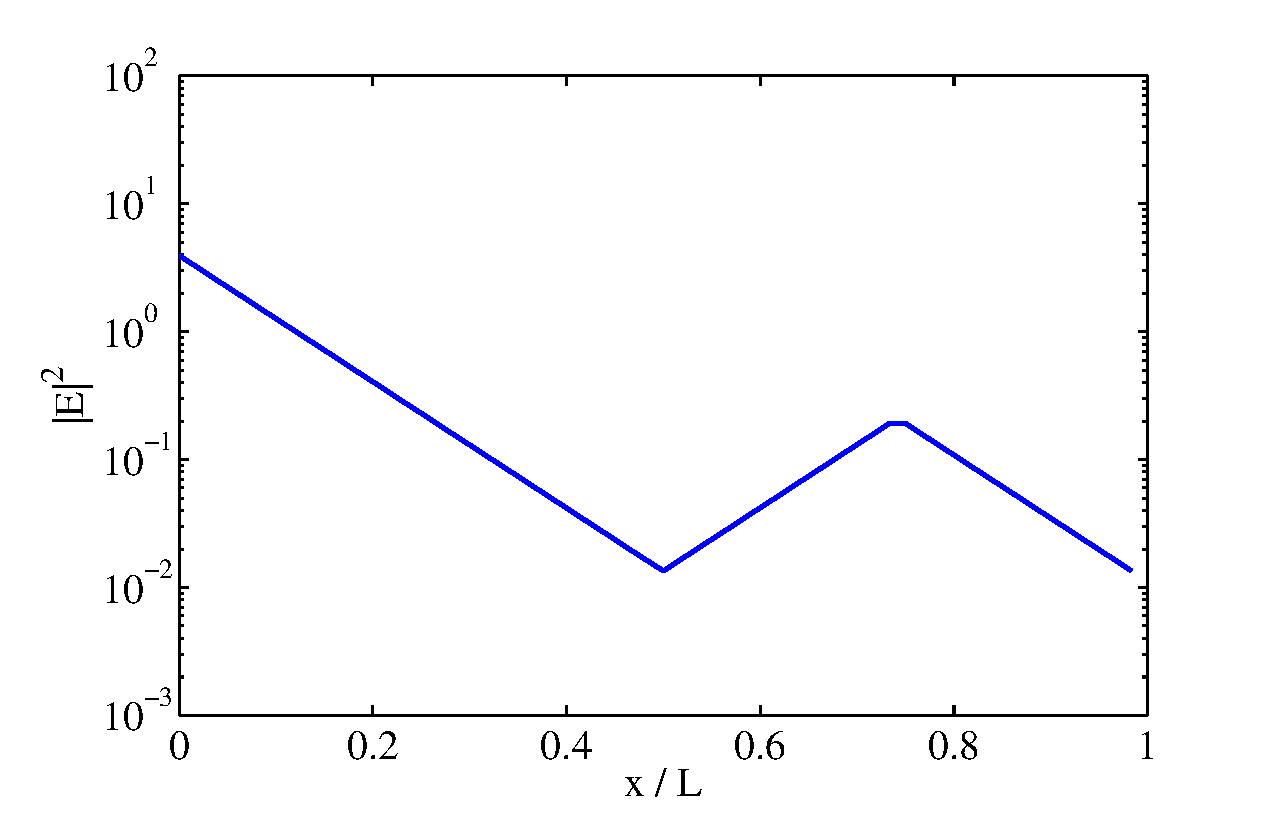
\includegraphics{pictures/passive_defect_34}}}
\vskip -0.5cm
\caption[The three plots correspond to a single defect at at $\frac{1}{4}$L, $\frac{1}{2}$L, and $\frac{3}{4}$L, respectively, for the passive periodic system
on semilogy scale (another analytical model).]{The three plots correspond to a single defect at at $\frac{1}{4}$L, $\frac{1}{2}$L, and $\frac{3}{4}$L, respectively, for the passive periodic system
on semilogy scale (another analytical model). We see the same
results we saw for Fig.~\ref{fig:barrierdefectlog} so
now we are confident that tunneling is causing the effect
seen in Fig.~\ref{fig:peaksmatchnotmatch}.}
%\label{fig:passivedefect}
\end{figure}
\end{comment}

These three models (random dielectric layers, potential barrier, and periodic layers) are closely related since all three are wave based.

Based on the passive analytical models we gain confidence that the light is tunneling through the material.  If there is a center of localization present in the random layers this is akin to the light tunneling to the potential well between the barriers and then tunneling out.

Also based on the analytical models we determine that the position of the center of localization/potential well/single defect directly affects how much energy is stored in the system.

\begin{comment}
\begin{figure}
\vskip -0.5cm
\centerline{
\scalebox{0.5}{\includegraphics{pictures/T_E_on_resonance_vs_xo}}}
\vskip -0.5cm
\caption[Transmission and energy and their ratio as a function of
the position of the center of localization.]{Transmission and energy and their ratio as a function of
the position of the center of localization. The energy plot is
similar to the theoretical energy in Fig.~\ref{fig:peaksmatchnotmatch}
As a result of the asymmetry in energy with respect
to defect position, the ratio of transmission to energy is not constant.}
\label{fig:defectpositionTE}
\end{figure}
\end{comment}

This variation of stored energy based on the position of
the center of localization explains why there are peaks
in energy but not always corresponding peaks in energy.
It also explains why peaks in energy imply peaks 
in transmission: the energy stored in the sample
means there is a center of localization in the sample, which
allows for increased transmission.  Now when we see a transmission and
energy plot versus frequency we can determine the location
of the center of localization by inspection.  If there is
a peak in transmission and energy,
then $ 0 < x < \frac{1}{2} L $.  If there is a peak
in transmission but not energy then the center of
localization is between $ \frac{1}{2} L < x < L $.

Presence of a center of localization for some frequency can be detected
through the deviations from a simple exponential 
decay in the field distribution inside the sample.

%%%%%%%%%%%%%%%%%%%%%%%%%%%%%%%%%%%%%%%%%%%%%%%%%%%%%%%%%
\subsubsection {Theory of Passive 1-D Systems}
%%%%%%%%%%%%%%%%%%%%%%%%%%%%%%%%%%%%%%%%%%%%%%%%%%%%%%%%%

% warning: the following figure may be redundant
% it is included for initial conceptual understanding

\begin{figure}
\vskip -0.5cm
\centerline{
\scalebox{0.9}{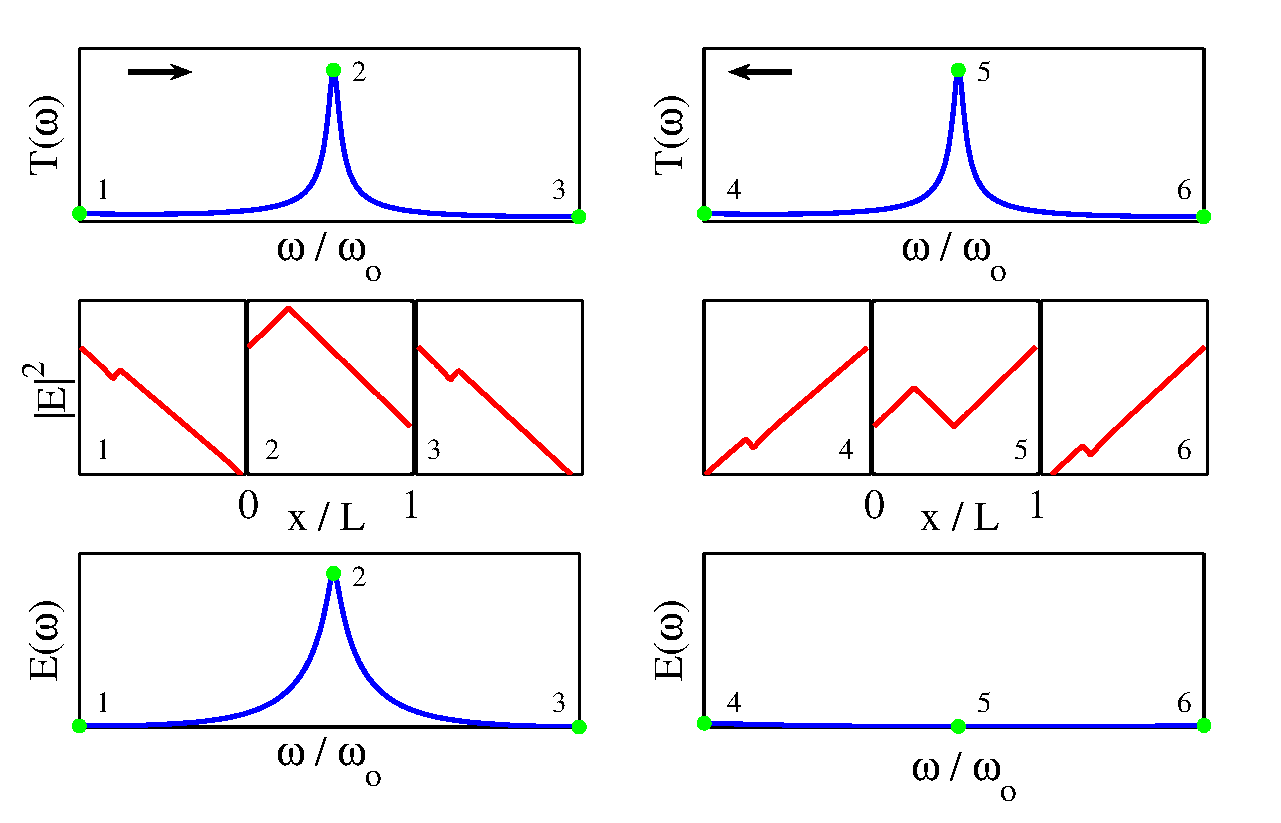
\includegraphics{pictures/peaks_match_peaks_dont_match}}}
\vskip -0.5cm
\caption[The above plots are from the periodic layers with
single defect model.]{The above plots are from the periodic layers with
single defect model. The left half are from the defect occuring
at $ \frac{1}{4} $L and the right set of plots are from the defect
at $ \frac{3}{4} $L, all without gain.  The top plot on both 
sides is transmission versus frequency centered at the resonant
frequency. For both $ \frac{1}{4} $L and $ \frac{3}{4} $L the resonant
frequency means a spike in transmission.  However, the lower plot
on both side (Energy versus frequency) shows that the amount of
energy is dependent on the defect position (which corresponds to
the center of localization in a random model).  Looking at
the behavior of the energy inside the sample for resonant
and off-resonant frequencies, the behavior of the wave changes
as close the resonant frequency. When off resonance there is
pure exponential decay, which translates to a straight decreasing
slope on the semilogy scale. On resonance there is a peak in energy
for both defect positions. However, the total energy in the sample
is much less for $ \frac{3}{4} $L (remember that these are semilogy
plots).  This demonstrates why T/${\cal E}$ is not constant in passive samples:
the ratio is affected by the position of the defect (center of localization
for random layers).}
%In the upper left figure we suppose there is 
%a peak in energy and corresponding peak in transmission.
%The amount of  energy in the sample is relatively large.
%In the upper right sketch we see what happens when 
%there is no peak in energy but there is a peak in transmission:
%much less energy is in the sample. 
%When the amount of energy in the media is plotted 
%as a function of center of localization, we see that there is an asymmetry.
%This is why T/${\cal E}$ is not smooth - it ratio is affected 
%by the position of the center of localization.}
\label{fig:peaksmatchnotmatch}
\end{figure}

We derive the T/${\cal E}$ ratio. The transmission T as a 
function of frequency $\omega$ and center of localization position $x_o$ 
is a lorentz distribution of the form

\begin{equation}
T = T(\omega, x_o) = \frac{(\exp(-\frac{L}{\xi}))^2}{ 
(\omega-\omega _o)^2 + (\exp(-\frac{L}{\xi})\frac{1}{2}\exp(\frac{\mid L-2 x_o \mid}{\xi}))^2 }
\label{eq:transmission}
\end{equation}
Where we have appoximated cosh() as $\frac{1}{2}\exp()$. 


From work done in Appendix B,
\begin{equation}
{\cal E}(x,\omega) = \frac{\xi}{2} ( T ( \exp\left(\frac{2(L-x_o)}{\xi}\right) - \exp\left(\frac{2(L-2 x_o+x_1)}{\xi}\right) + \exp\left(\frac{2(L-x_o))}{\xi}\right) -1 ) + 4 (1-\exp\left(-\frac{2 x_1}{\xi}\right)) )
\label{fig:energy}
\end{equation}

As a check on Energy we can look at the resonant frequencies as the center of localization position $x_o$ varies. We recover Fig.~\ref{fig:energydistrib}.

\begin{figure}
\vskip -0.5cm
\centerline{
\scalebox{0.5}{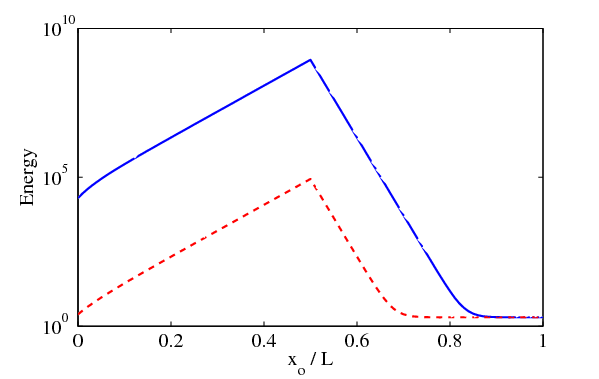
\includegraphics{pictures/energy_distribution_g0_and_99gc}}}
\vskip -0.5cm
\caption{Energy distribution as a function of position of center
of localization $x_0$ on resonant frequencies without gain (dotted
red) and with 99\% of critical gain (upper solid blue). See 
Eq.~\ref{fig:energy}. These
plots show why the peaks in transmission do not always have a corresponding
peak in energy, as seen in Fig.~\ref{fig:peaksmatchnotmatch}. and 
Fig.~\ref{fig:tenkenergytransmission}. Even when gain is added the 
asymmetry does not go away.}
\label{fig:energydistrib}
\end{figure}

Now we will look only at resonant frequencies
($\omega = \omega_0$) with sufficient gain that $x_1$ goes to zero (then
$y_2$ has a range from zero to $x_1$. This includes passive systems where the defect is in
the first half of the sample and if the defect is in
the second half, then the gain is sufficient that there 
is no initial exponential decay regardless of defect position. Visually, the plot has a single clusp.  

\begin{equation}
\frac{\cal E}{T} = \frac{\xi}{2} ( 2 \exp\left(\frac{2(L-x_0)}{\xi}\right) - \exp\left(\frac{2(L-2 x_0)}{\xi}\right) -1 ) )
\end{equation}

\begin{figure}
\vskip -0.5cm
\centerline{
\scalebox{0.5}{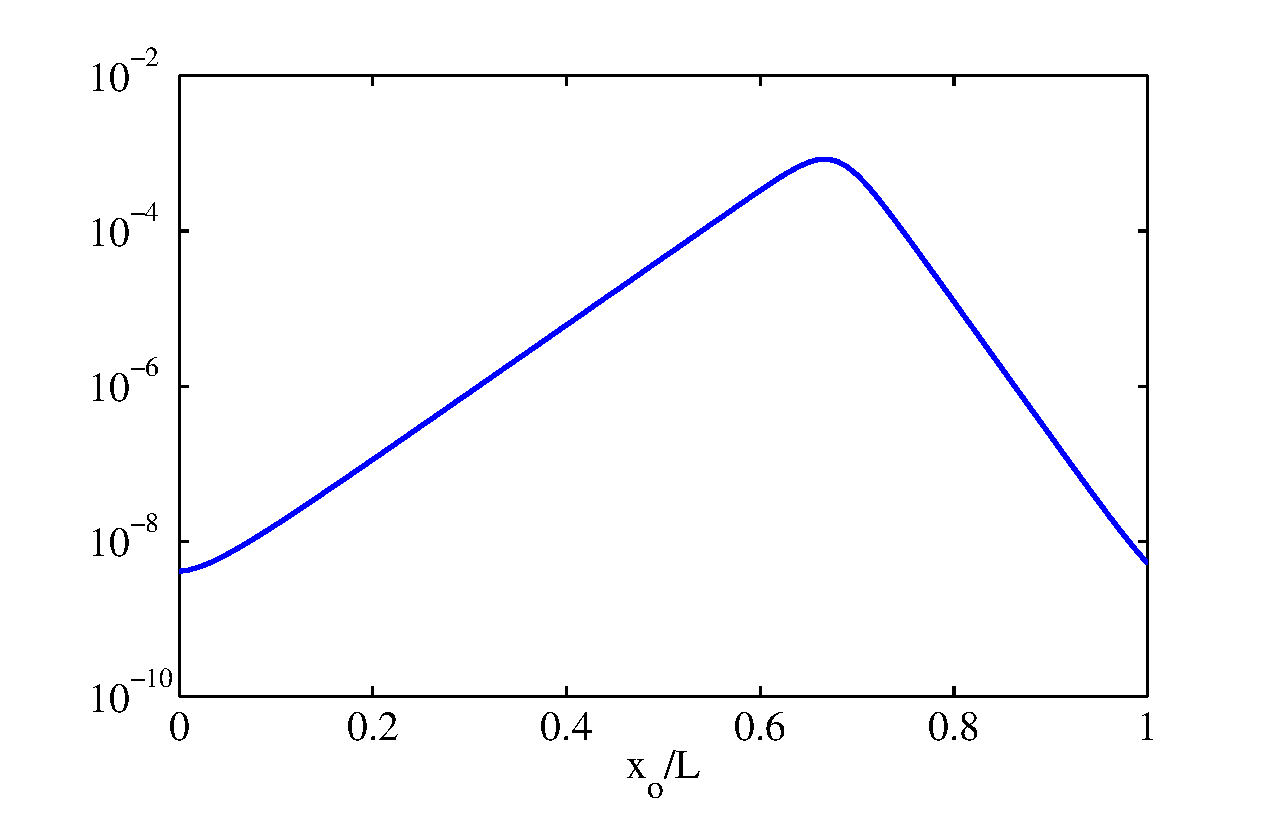
\includegraphics{pictures/log_TE_v_defect_position_passive}}}
\vskip -0.5cm
\caption{Transmission/Energy as a function of position of center
of localization $x_0$ on resonant frequencies without gain. Eq.~\ref{fig:energy}
divided by Eq.~\ref{fig:correctedtransmission}. This is why T/${\cal E}$ will not work
for a criteria; the ratio depends on where the center of localization occurs. 
One can not average over all possible positions.}
\label{fig:energytranspassive}
\end{figure}

If we assume $x_0$ is not near the edges of the sample $x_0 > 0$ and $x_0 < L$ with $L > \xi$ then we can drop the last two terms, leaving
\begin{equation}
\frac{\cal E}{T} = \xi \exp\left(\frac{2(L-x_0)}{\xi}\right)
\end{equation}

Inverting that to get T/${\cal E}$,

\begin{equation}
\frac{T}{\cal E} = \frac{1}{\xi} \exp\left(-\frac{2(L-x_o)}{\xi}\right)
\end{equation}

Note that the log of either results in a non-exponential form which could be integrated. Neither T/${\cal E}$ nor ${\cal E}$/T is particularly useful. When one averages ${\cal E}$/T the background dominates, whereas for T/${\cal E}$ the resonant frequency behavior dominates. See Fig.~\ref{fig:logTEET}.

\begin{figure}
\vskip -0.5cm
\centerline{
\scalebox{0.5}{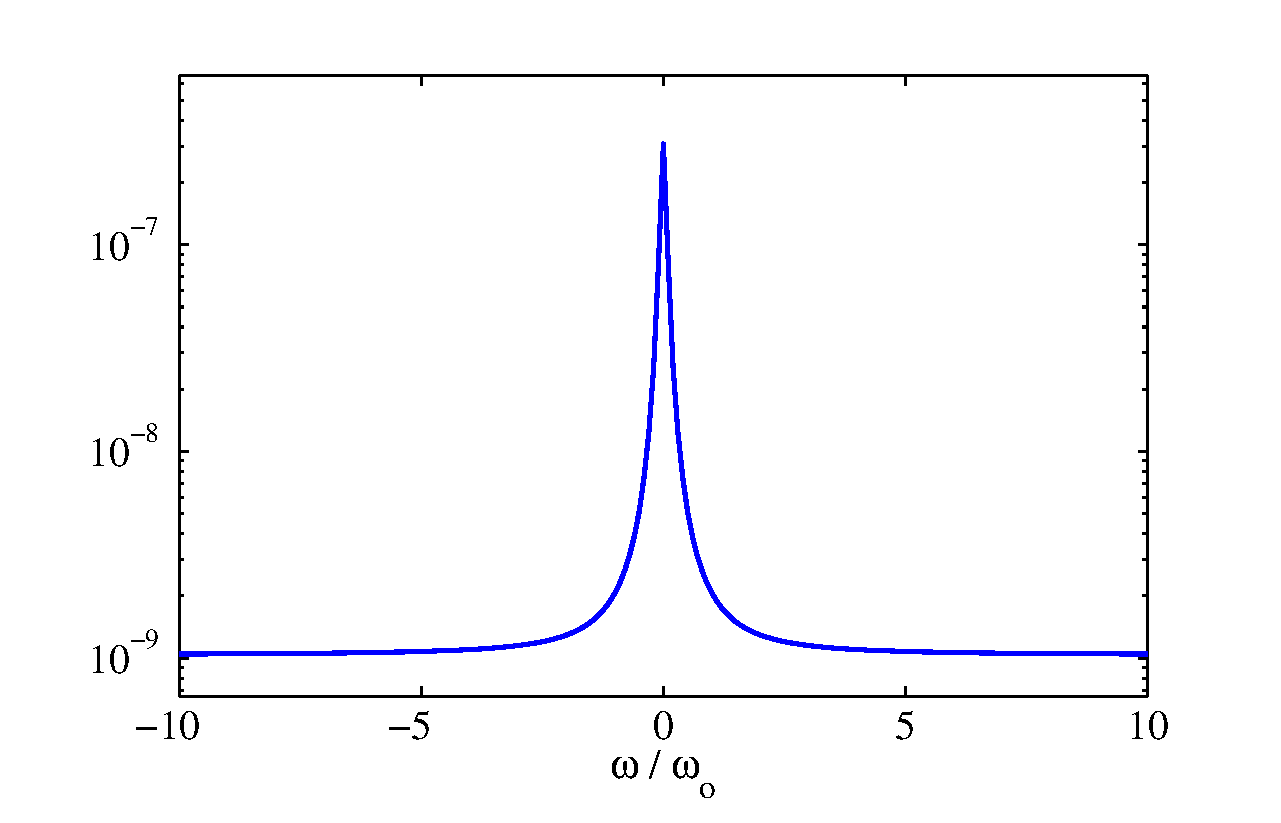
\includegraphics{pictures/log_TE_v_freq}}}
\vskip -0.5cm
\caption{T/${\cal E}$ versus frequency for passive systems
with the correction from Eq.~\ref{fig:correctedtransmission}. Frequency 
is zero on resonance. This plot show that
if T/${\cal E}$ is attempted to be used as a criteria for 
finding localization for an ensemble of samples, the peak and background
obsure each other. The problem is the same for ${\cal E}$/T.}
\label{fig:logTEET}
\end{figure}

When gain is added, the left boundary condition ($y_1=4$ at $x=0$) is no
longer valid. The entire field distribution grows in height, including
the end points. This would be equivalent to letting $x_1$ (the turning
point) become negative, which is non-physical. In order to prevent this
we change the limits of integration to be max($x_1$,0) instead of $x_1$ 
in Eq.~\ref{fig:Eintegral}.

Another problem arises with T from Eq.~\ref{eq:transmission} in 
that the ``worst case'' (minimum for T) is when we are so far off resonance
that only exponential decay occurs. As the above equations are given
T goes to zero, which is incorrect. Physically, T asymptotically reaches the exponential
decay value. Thus in order to make this correction, we shift the 
Eq.~\ref{fig:transmission} up by the exponential decay background.

\begin{equation}
T = T(\omega, x_0) = \frac{(\exp(-\frac{L}{\xi}))^2}{
(\omega-\omega _0)^2 + (\exp(-\frac{L}{\xi})\frac{1}{2}\exp(\frac{\mid L-2 x_0 \mid}{\xi})-g)^2
} + \exp\left(-\frac{L}{\xi}\right)^2
\label{fig:correctedtransmission}
\end{equation}

%%%%%%%%%%%%%%%%%%%%%%%%%%%%%%%%%%%%%%%%%%%%%%%%%%%%%%%%%
\subsubsection {Adding Gain}
%%%%%%%%%%%%%%%%%%%%%%%%%%%%%%%%%%%%%%%%%%%%%%%%%%%%%%%%%

Now we understand why the ratio of transmission to energy (T/${\cal E}$) is not smooth in passive systems: the ratio depends on the position of the center of localization. When gain is added to the random system we hope that T/${\cal E}$ becomes smoother because we do not expect such a dramatic dependence on the position of the localization center.

In order to reach the critical gain we investigate the periodic system with single defect. We did not test the addition of gain in the double potential single well model.

When gain is added to the three canonical cases we see a rise in the peaks and the peak position remains the same. The tail for the $ \frac{3}{4} $L does not change, only the peak increases.  (Fig.~\ref{fig:periodicdefect}).

\begin{figure}
\vskip -0.5cm
\centerline{
\scalebox{0.3}{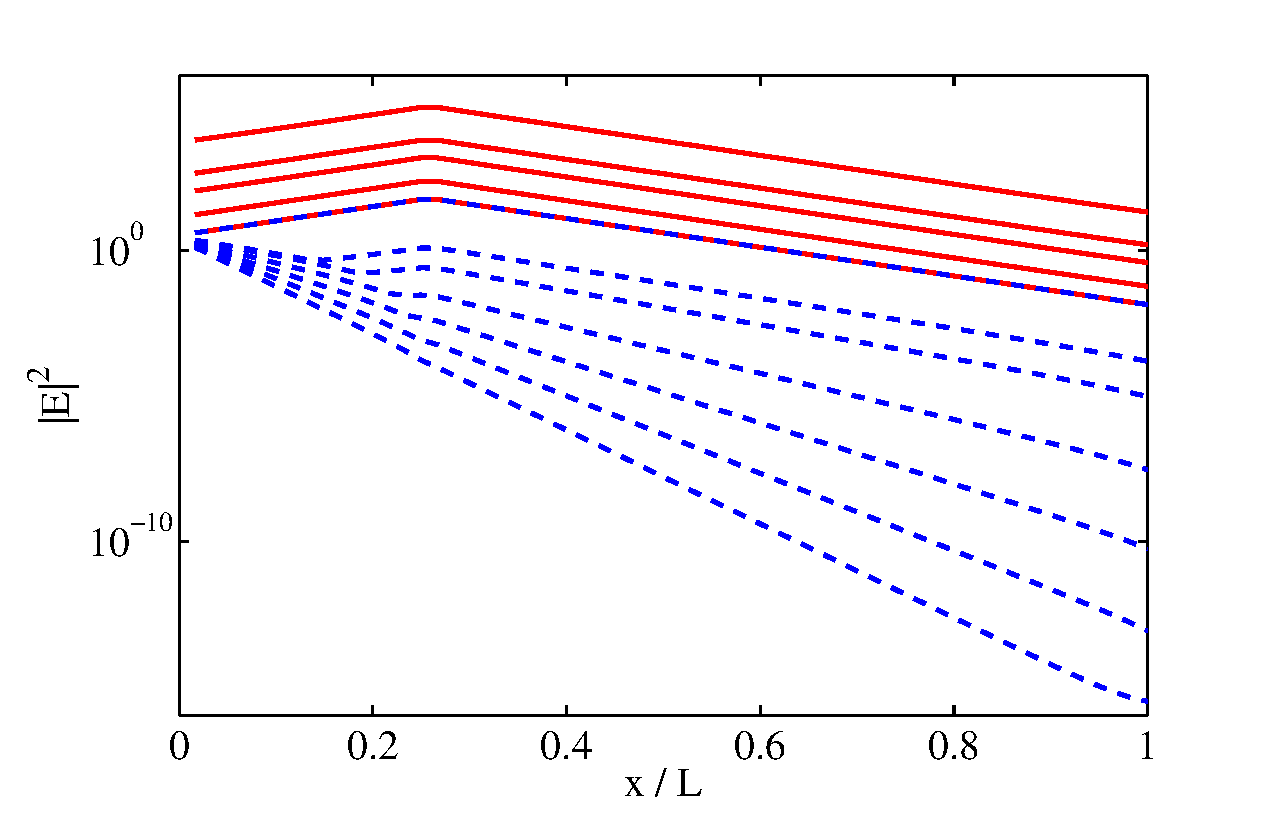
\includegraphics{pictures/periodic_14_defect_absorb_to_gain}}
\scalebox{0.3}{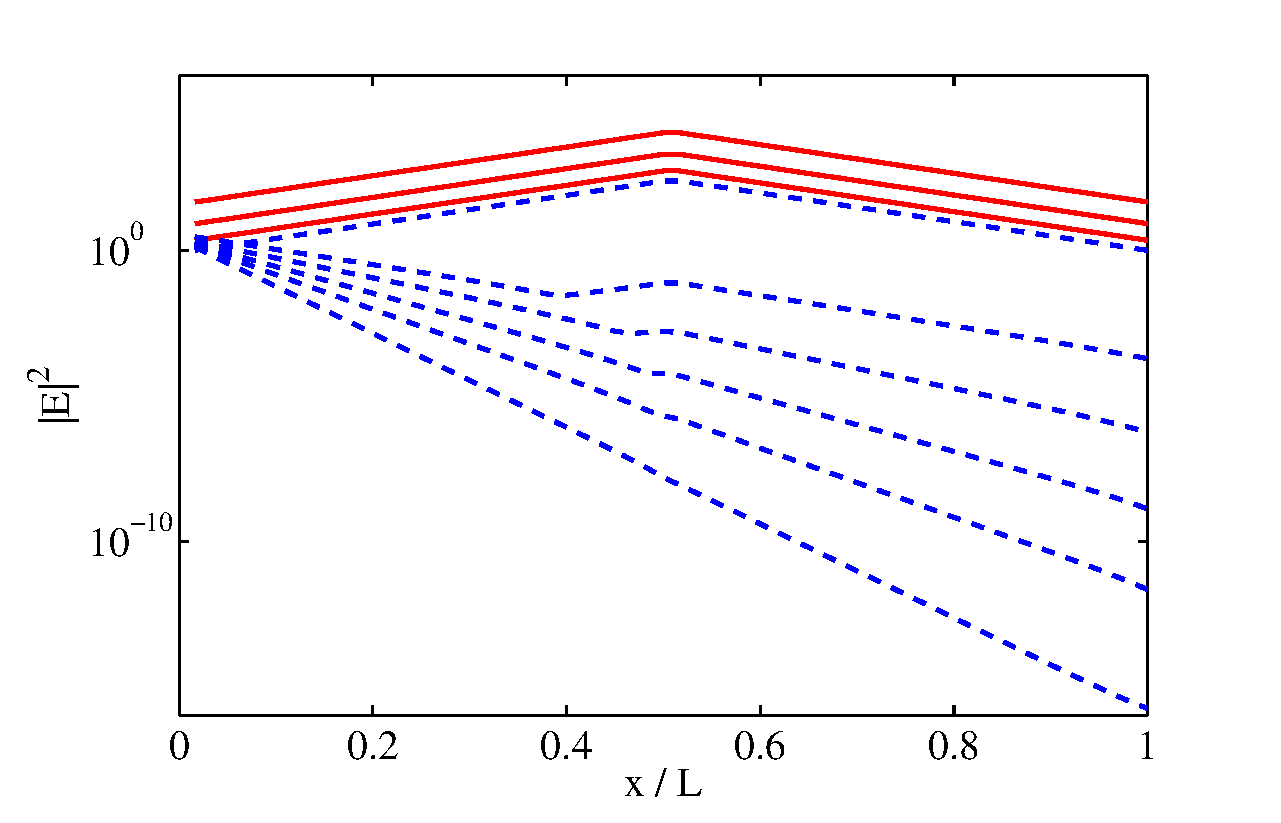
\includegraphics{pictures/periodic_12_defect_absorb_to_gain}}
\scalebox{0.3}{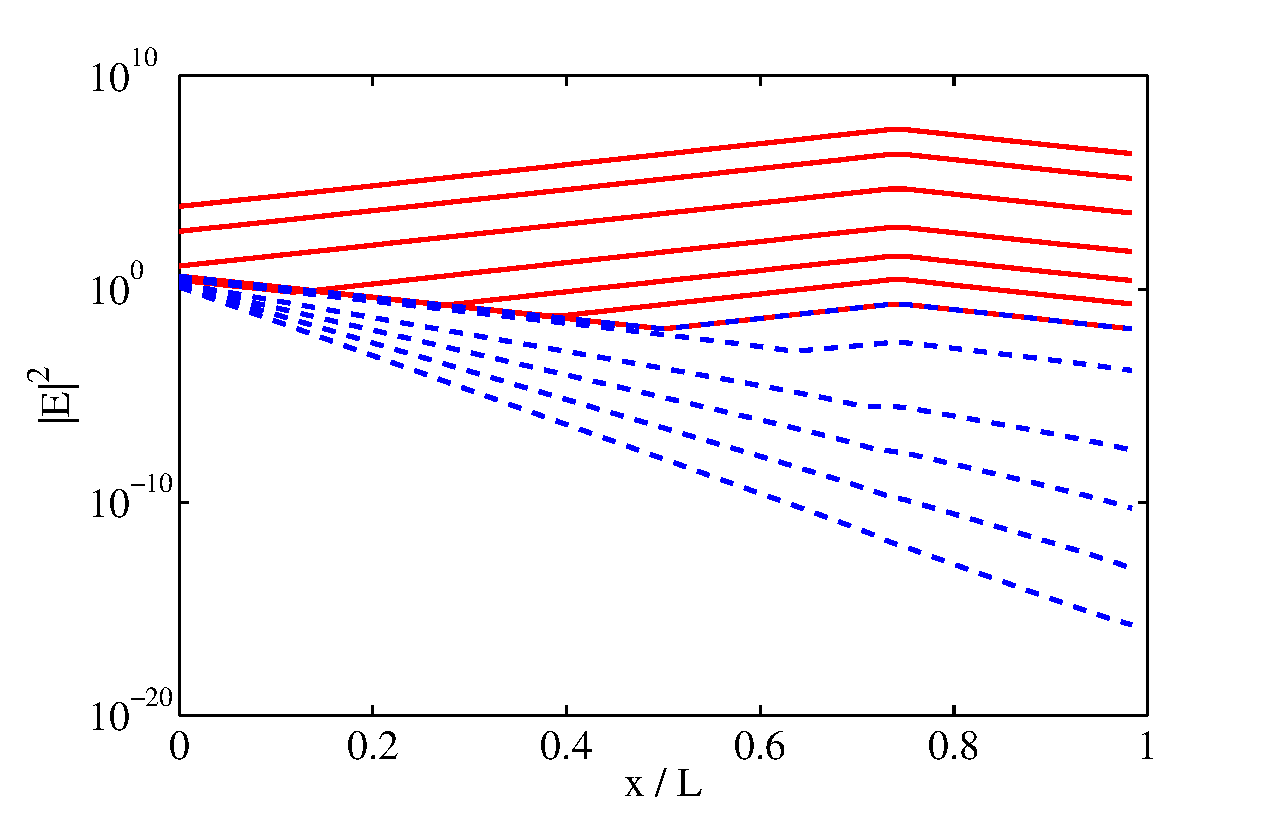
\includegraphics{pictures/periodic_34_defect_absorb_to_gain}}}
\vskip -0.5cm
\caption[The log of the field in the sample for three canonical positions for the periodic 1-D structure with single defect.]{The log of the field in the sample for three canonical positions for the periodic 1-D structure with single defect. In this analytical model the single anomalous layer is at $ \frac{1}{4} $L, $ \frac{1}{2} $L, and $ \frac{3}{4} $L, respectively and the amount of absorption or gain is varied. The lowest dotted blue straight line is full absorption. On a log scale the exponential scale appears as a more obvious straight negative slope line. As absorption is decreased and the passive system is approached a turning point appears. For the $ \frac{1}{4} $L and $ \frac{1}{2} $L systems this turning point disappears at the passive system incident side. Then gain is added to the model (solid red line). For the $ \frac{1}{4} $L and $ \frac{1}{2} $L defects the peak simply increases, as expected in active media. For the $ \frac{3}{4} $L system the turning point moves toward the incident side. Thus in active media the wave form changes for defects occuring in the second half of the sample. Eventually the gain is sufficient that the $ \frac{3}{4} $L position is symmetric with the  $ \frac{1}{2} $L position. Now in all three canonical positions with gain the field in the sample grows exponentially to a peak before falling.}
%The analytical periodic model with defects at . We scan from the absorption (blue) regime
%to gain (red).}
\label{fig:periodicdefect}
\end{figure}

Note that near the critical gain, the transmission and the field distribution inside the sample becomes very sensitive to the amount of gain added to the system. %[foreshadowing.]

At the critical gain the defect at $ \frac{1}{4} $L and the
defect at $ \frac{3}{4} $L
cases are symmetric with respect to each other about the y axis.
The defect at $ \frac{1}{2} $L is symmetric about x=$ \frac{1}{2} $L
and the defect at $ \frac{1}{4} $L would be symmetric
with the defect at $ \frac{3}{4} $L if
it were flipped around. [Foreshadowing, we will get back to this.]

At the critical gain the ratio of transmission to energy
is smoother than the passive system,
but there are some issues for when the center of
localization is between $ \frac{1}{2}$L and L. We have
found that T/${\cal E}$ is
a ``good'' parameter for 1-D systems with gain, in that it is
not divergent (unlike T and ${\cal E}$ are separately).  It can be
measurable.  However, it is not perfect as it depends on sample orientation.

%%%%%%%%%%%%%%%%%%%%%%%%%%%%%%%%%%%%%%%%%%%%%%%%%%%%%%%%%
\subsubsection {Closed and Open Systems Theory for Passive 1D Models}
%{closed and open systems: the importance of phase}
%%%%%%%%%%%%%%%%%%%%%%%%%%%%%%%%%%%%%%%%%%%%%%%%%%%%%%%%%

The idea of flipping the sample orientation warrants
attention.  If there is a center of localization
at $ \frac{1}{4} $L and
the sample is flipped (sample goes from L to 0 instead
of the standard 0 to L) then we know there will be a center
of localization at $ \frac{3}{4} $L.  The waveform for
these two localization centers is the same in the region
of localization.

An equivalent to flipping the sample orientation is
to change the orientation of the light.  If one keeps
the sample fixed and shines light on the x=L side of the
sample then we get the same result as fixing the light and
flipping the sample orientation.  The math is slightly
different for the two cases. %As flipping the light source
%is more common in literature we will stick with that.

We will call the case where light is incident on the left side ``LR''
as light moves left to right. Conversely we will call the
light being incident on the right side ``RL''.  Also,
we will call the resulting LR field 
distribution $ \psi _1(x) $ and the RL wave $ \psi  _2(x) $. 
The flipping we will term ``reciprocity.'' 

A reality check for flipping the sample (or flipping the
light source) is that the transmission should be the same for the
two cases since the light is traveling through the
same material.  Note that flipping both the sample and the
light gets one back to the original setup.

Thouless criteria says that a small change in boundary
conditions should not affect energy spectrum. However, we 
find that flipping the beam (which is a small change
in boundary conditions) does cause an enormous 
change {\it in the waveform in the sample}. This  affects
how much energy is in the system, ie the waveform for
localization at $ \frac{1}{4} $L becomes the
waveform for localization at $ \frac{3}{4} $L.
There is a lot less energy in the system for the
$ \frac{3}{4} $L waveform as compared to $ \frac{1}{4} $L. A
small change in the boundary conditions leads to
a significant change in how much energy is stored
in the sample.

How can reciprocity help to identify localization? Experimentally one can shine light on either side of a given sample, so reciprocity is straight forward to execute.  What follows is	% don't tell experimentalist what is "easy"
the mathematical analysis of using reciprocity.

We start by showing that the two wave forms are functionally independent by finding the Wronskain for the left sides of the two orientations. It can be shown that for our Maxwell equation the Wronskian is position independent.
 % see notes 20080117

\begin{figure}
\vskip -0.5cm
\centerline{
\scalebox{0.8}{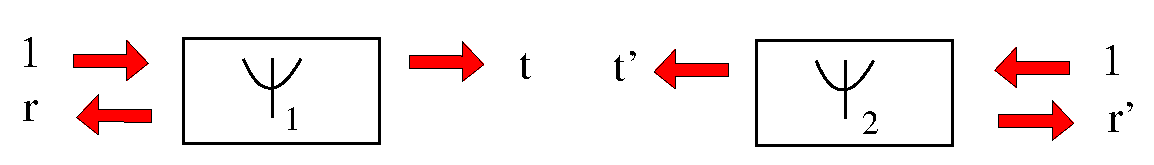
\includegraphics{pictures/wronskian_LR_RL}}}
\vskip -0.5cm
\caption[For the two orientations, left-to-right and right-to-left, two wave functions are assigned: $ \psi _1$ and $ \psi _2$.]{For the two orientations, left-to-right and right-to-left, two wave functions are assigned: $ \psi _1$ and $ \psi _2$. The wronskian for is the same for both since the transmission is the same for both orientations.}
\label{fig:wronskainLRRL}
\end{figure}

\begin{equation}
\begin{vmatrix}
1 \exp(i k x) + r \exp(-i k x) & t' \exp(-i k x) \\
i k \exp(i k x) - i k r \exp(-i k x) & i k t' \exp(i k x)
\end{vmatrix}
 = -2 i k t'
\label{eq:wronskleft}
\end{equation}

Similarly, the Wronskain for the right sides is: % semi-redundant

\begin{equation}
\begin{vmatrix}
 t \exp(i k x) & 1 \exp(-i k x) + r' \exp(i k x)\\
i k t \exp(i k x) & -i k \exp(-i k x) + i k r' \exp(-i k x)
\end{vmatrix}
 = -2 i k t
 \label{eq:wronskright}
\end{equation}

Note that the two Wronskians are non-zero and are the same since t = t'. Now that we have to independent functions we can use them as a basis to create a new linear combination.

An analog is the one dimensional potential well with an eigen state in the well.In a closed system we can find eigen states and eigen frequencies.  For the passive random model this would be equivalent to adding mirrors to the edges of the sample so that no light escapes to the environment.

For the open system (both for potentials and in the case we are working with, layers of dielectric) there will be two solutions, a left and right traveling wave.  For closed systems there is one solution (composed of two waves - standing wave).

Closed system solution can be expressed in terms of $\psi _1(x), \psi _2(x)$:
\begin{equation}
\psi (x) = c_1  \psi _1(x) + c_2  \psi _2(x)
\end{equation}
%   Y(x) = c_1 Y_1(x) + c_2 Y_2(x)
where $\psi _1$ and $ \psi  _2 $ are the wave functions associated with the LR and RL orientations in the random system. To find the eigenstates apply the boundary conditions: the function $\psi$(x) is zero at the edges of the closed system. 
\begin{equation}
\begin{gathered}
\psi (x=0) = c_1  \psi _1(0) + c_2  \psi _2(0) = 0 \\
\psi (x=L) = c_1  \psi _1(L) + c_2  \psi _2(L) = 0
\end{gathered}
\end{equation}
%  Y(0) = c_1 Y_1(0) + c_2 Y_2(0) = 0
%  Y(L) = c_1 Y_1(L) + c_2 Y_2(L) = 0
This can only be valid when the determinant is zero
\begin{equation}
det
\begin{bmatrix}
\psi _1(0) & \psi _2(0) \\
\psi ' _1(L) & \psi ' _2(L) 
\end{bmatrix}
 = 0
\end{equation}

This $ \psi _1 $ and $ \psi _2 $ can be interpreted as either the electric field at the edges or related to the reflection and transmission coefficients:
\begin{equation} % see notes 20080130
\begin{gathered}
E(0) =  \psi _1 (0) = 1+r \\
k E'(0) = \psi ' _1 (0) = k i (1-r)
\end{gathered}
\end{equation}
or equivalently t t' - (1+r) (1+r') = 0. %notes 20080117 last page

Now we can go back to the random system and find the determinant given $\psi  _1$(x) and $\psi _2 $(x). When the determinant is zero that implies the frequency is an eigen frequency (in a closed system) and the wave function is an eigenstate.  Since the layers actually make an open system, we will call these ``resonant frequencies.'' Scanning the range of frequencies yields points on the T and ${\cal E}$ versus frequency plot that correspond (perfectly) with the peaks in energy in transmission.

Note that when the transmission and energy versus frequency is plotted then the transmission for the LR and RL cases is the same (t=t'), whereas the energy is not the same for the LR and RL orientation. The energy peaks at different frequencies, resulting in two lines for energy, whereas there is one for transmission.  The dots are where the determinant is zero.

\begin{figure}
\vskip -0.5cm
\centerline{
\scalebox{0.5}{\includegraphics{pictures/trans_energy_det}}} 
\vskip -0.5cm
\caption[Transmission, energy, and determinant=0 for LR and RL orientations versus frequency.]{Transmission, energy, and determinant=0 for LR and RL orientations versus frequency. This is similar to Fig.~\ref{fig:tenkenergytransmission}, except now we can predict where the peaks occur.}
\label{fig:energytransmissiondet}
\end{figure}
We can test that the states at these resonant frequencies are orthogonal. See Deych's paper\cite{2005_Deych}.
% see notes 20080214
\begin{equation}
\frac{\int _0 ^L \psi _1 \psi _2 ^* \epsilon(x) dx}
{\sqrt{\int _0 ^L \psi _1 \psi _1 ^* \epsilon(x) dx}
 \sqrt{\int _0 ^L \psi _2 \psi _2 ^* \epsilon(x) dx}} = 0
\end{equation}

%20080213 page 1
Note that when the center of localization is at $ \frac{1}{4} $L for resonant frequencies the electric field at x=0 is close to zero.  (See Fig.~\ref{fig:standingwave}.) Reason: the waves outside the material are cancelling out due to interference.  This results in a standing wave.   r=-1 (from 1+r=0).

\begin{figure}
\vskip -0.5cm
\centerline{
   \scalebox{0.5}{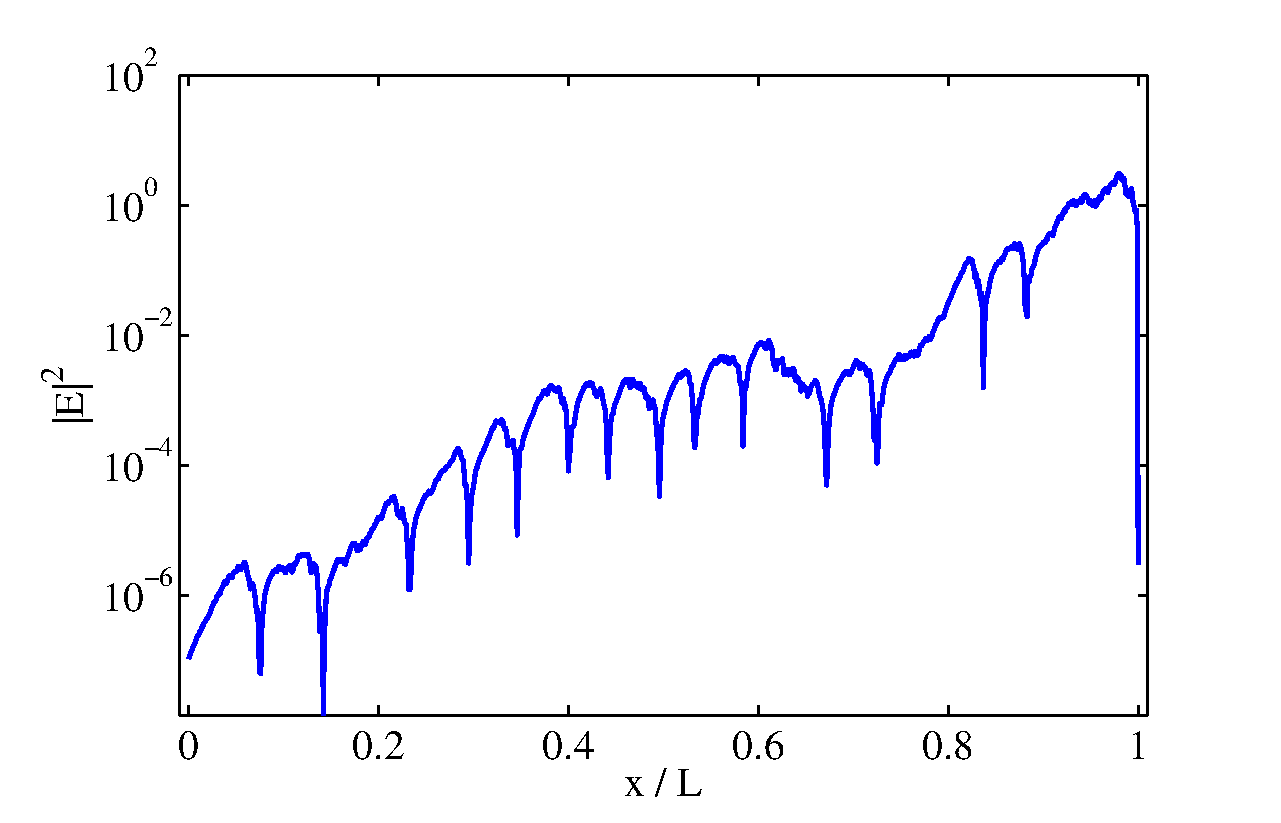
\includegraphics{pictures/standing_wave_electric_field}}
}
\vskip -0.5cm
\caption[A resonant frequency showing drop-off at x=L.]{A resonant frequency showing drop-off at x=L. Even though the center of localization may not be obvious for this resonant frequency, the fact that the electric field approaches zero on both sides of the sample means the field is approaching a closed system resonance.}
\label{fig:standingwave}
\end{figure}

This is a reliable and accurate method for find lasing threshold in computational models. To find the critical gain first find a resonant frequency by calculating where the determinant is zero. Then for each resonant frequency plot the transmission versus gain. The transmission will diverge at critical gain. The amount of gain added becomes very sensitive near the critical gain, but one can find arbitrarily small bounds on what the critical gain is by zooming in on the peak.

An alternative method for finding the critical gain is to look at the transmission versus frequency plot and measure the full width at half maximum (FWHM), $\gamma$.
\begin{equation}
g_{critical} = \frac{\gamma}{2} / \frac{2 \pi}{ \lambda }
% old: \frac{\frac{\gamma}{2}}  {\frac{2 \pi}{ \lambda }}
\end{equation}

Experimentally the light has to be shone from both left-to-right and right-to-left, but the result is to find what would be eigen frequencies of the closed system.  We will still call these the resonant frequencies since we are in the open system.

As a reality check, the wave coefficients A and B should be equal throughout the sample at resonant frequencies since the left and right-traveling waves are equal (see Fig.~\ref{fig:ABLRRLlog}.  A=B also implies that there is no oscillation in energy at the resonant frequency, thus there is no energy leakage out of the sample.

If A=B then the two complex waves should sum to a real wave:
\begin{equation}
A \exp(i k x)+A \exp(-i k x) = A \cos(k x)
\end{equation}

\begin{figure}
\vskip -0.5cm
\centerline{\scalebox{0.8}{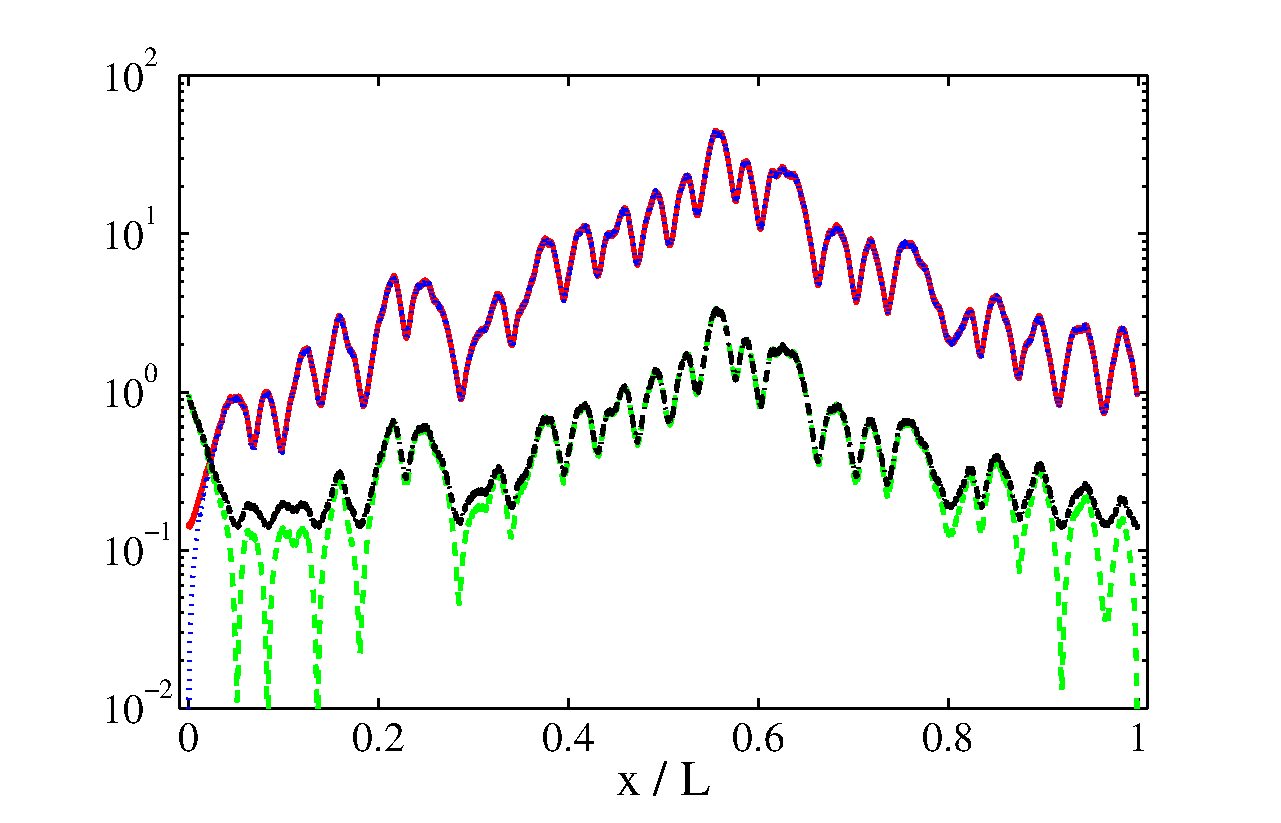
\includegraphics{pictures/AB_LR_and_RL}}}
\vskip -0.5cm
\caption[A and B coefficients for the two orientations (left to right and right to left).]{A and B coefficients for the two orientations (left to right and right to left). The lower two lines (dotted green and dotted black) are the backward (B) and forward (A) propagation coeffients, respectively of the electric field for the left-to-right orientation (both start out near unity on the incident side). The forward propagation A is non-zero on the transmission side of the sample and dotted green B falls to zero. The upper red and blue lines are hard to distinguish through most of the sample because they overlap. The red and blue lines are A and B for the right-to-left orientation since both start out near unity on the right side and only near the transmission side does it become apparent that the solid red is forward propagating A whereas dotted blue falls to zero and is the B coefficient. There is very little difference between A and B for each orientation which means there is little energy difference in the two wave directions. Normally for non-resonant frequencies A and B are very different.}
\label{fig:ABLRRLlog}
\end{figure}


Claim: the standing wave has constant phase throughout the sample %[so far unsubstantiated in our models]. 
[We should go back and study this.]

%%%%%%%%%%%%%%%%%%%%%%%%%%%%%%%%%%%%%%%%%%%%%%%%%%%%%%%%%
\subsubsection{Overview of Finding Criteria for Localization}
%%%%%%%%%%%%%%%%%%%%%%%%%%%%%%%%%%%%%%%%%%%%%%%%%%%%%%%%%

In forming a criteria for localization (in both passive systems and systems with gain) it is important to remember what distinguishes localization from diffusion.  The diffusion equation does not keep track of phase, thus it can not account for localization, which is a result of wave interactions with phase.  Regardless of whether one is in the absorption, passive, or active system, a criteria for localization needs to be able to account for phase.  Constant phase means there is a center of localization occurring.  Since phase is not (?) an experimentally measurable quantity then the criteria is going to need to be able to be dependent on or directly related to phase.

%%%%%%%%%%%%%%%%%%%%%%%%%%%%%%%%%%%%%%%%%%%%%%%%%%%%%%%%%
\subsubsection{Add gain to random 1-D model}
%%%%%%%%%%%%%%%%%%%%%%%%%%%%%%%%%%%%%%%%%%%%%%%%%%%%%%%%%

In the passive system $ \psi _1 $ and $ \psi _2 $ form an orthonormal basis for $ \psi $(x) where $ \psi _1 $ and $ \psi _2 $ refer to the two orientations for shining light on the sample, left-to-right and right-to-left, respectively.

When gain is added to the system, we have a new $\tilde{\psi}$ which depends on the gain:
\begin{equation}
\tilde{\psi}(x,g) = \alpha(g)  \psi _1(x) + \beta(g)  \psi _2(x)
\end{equation}
Where we can find the complex coefficients
$\alpha$ and $\beta$ from
\begin{equation}  % see notes 20080225
\begin{gathered}
\beta _1 = \frac{\int _0 ^L \psi _1 \tilde{\psi _1 ^*} \epsilon(x) dx}
{\sqrt{\int _0 ^L \psi _1 \psi _1 ^* \epsilon(x) dx}
 \sqrt{\int _0 ^L \tilde{\psi _1} \tilde{\psi _1 ^*} \epsilon(x) dx}} \\
\alpha _1 = \frac{\int _0 ^L \psi _2 \tilde{\psi _1} \epsilon(x) dx}
{\sqrt{\int _0 ^L \psi _2 \psi _2 ^* \epsilon(x) dx}
 \sqrt{\int _0 ^L \tilde{\psi _1} \tilde{\psi _1 ^*} \epsilon(x) dx}}
\end{gathered}
\end{equation}

The coefficients depend on the orientation of the light, so there is another set of coefficients for the other orientation. Similarly for $ \beta _2 $ and $ \alpha _2 $,
\begin{equation}  % see notes 20080225
\begin{gathered}
\beta _2 = \frac{\int _0 ^L \psi _1 \tilde{\psi _2 ^*} \epsilon(x) dx}
{\sqrt{\int _0 ^L \psi _1 \psi _1 ^* \epsilon(x) dx}
 \sqrt{\int _0 ^L \tilde{\psi _2} \tilde{\psi _2 ^*} \epsilon(x) dx}} \\
\alpha _2 = \frac{\int _0 ^L \psi _2 \tilde{\psi _2} \epsilon(x) dx}
{\sqrt{\int _0 ^L \psi _2 \psi _2 ^* \epsilon(x) dx}
 \sqrt{\int _0 ^L \tilde{\psi _2} \tilde{\psi _2 ^*} \epsilon(x) dx}}
\end{gathered}
\end{equation}
A reality check on $\alpha$ and $\beta$ is that
\begin{equation}
\| \alpha \| ^2 + \| \beta \| ^2= 1
\end{equation}

These two sets of coefficients can be plotted with respect to gain. We scan gain (by adding complex refractive index) from zero (passive systems) up to the critical gain. 
\begin{figure}
\vskip -0.5cm
\centerline{
\scalebox{0.3}{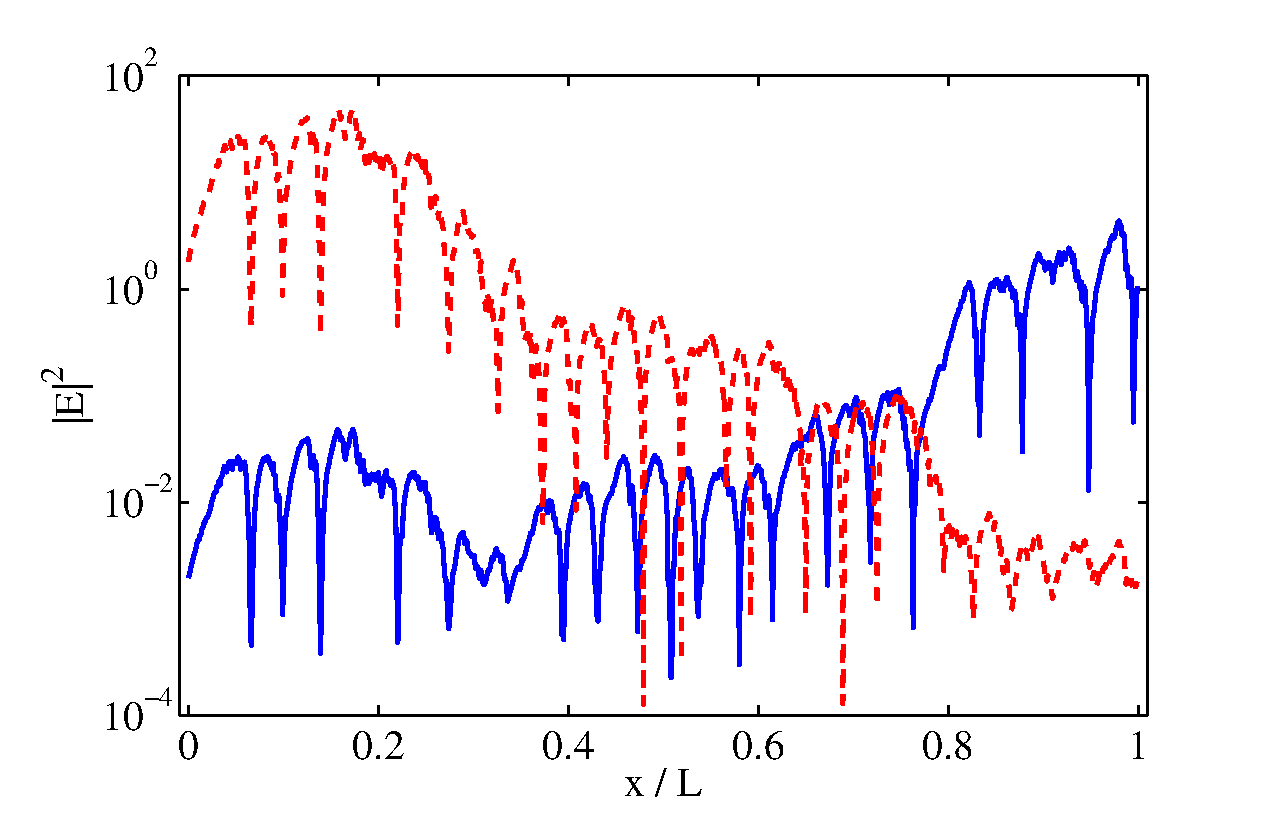
\includegraphics{pictures/alpha_beta_electric_field}}
\scalebox{0.3}{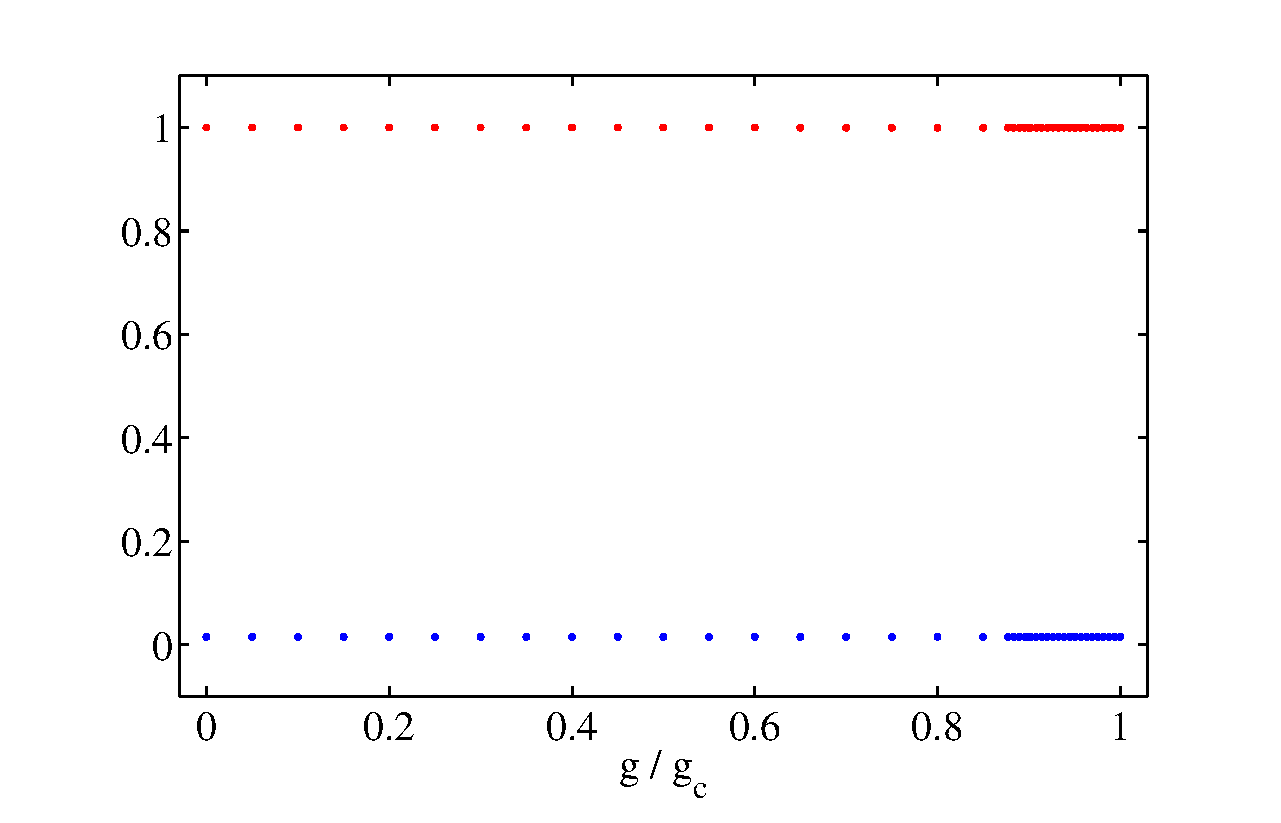
\includegraphics{pictures/alpha2_beta2}}
\scalebox{0.3}{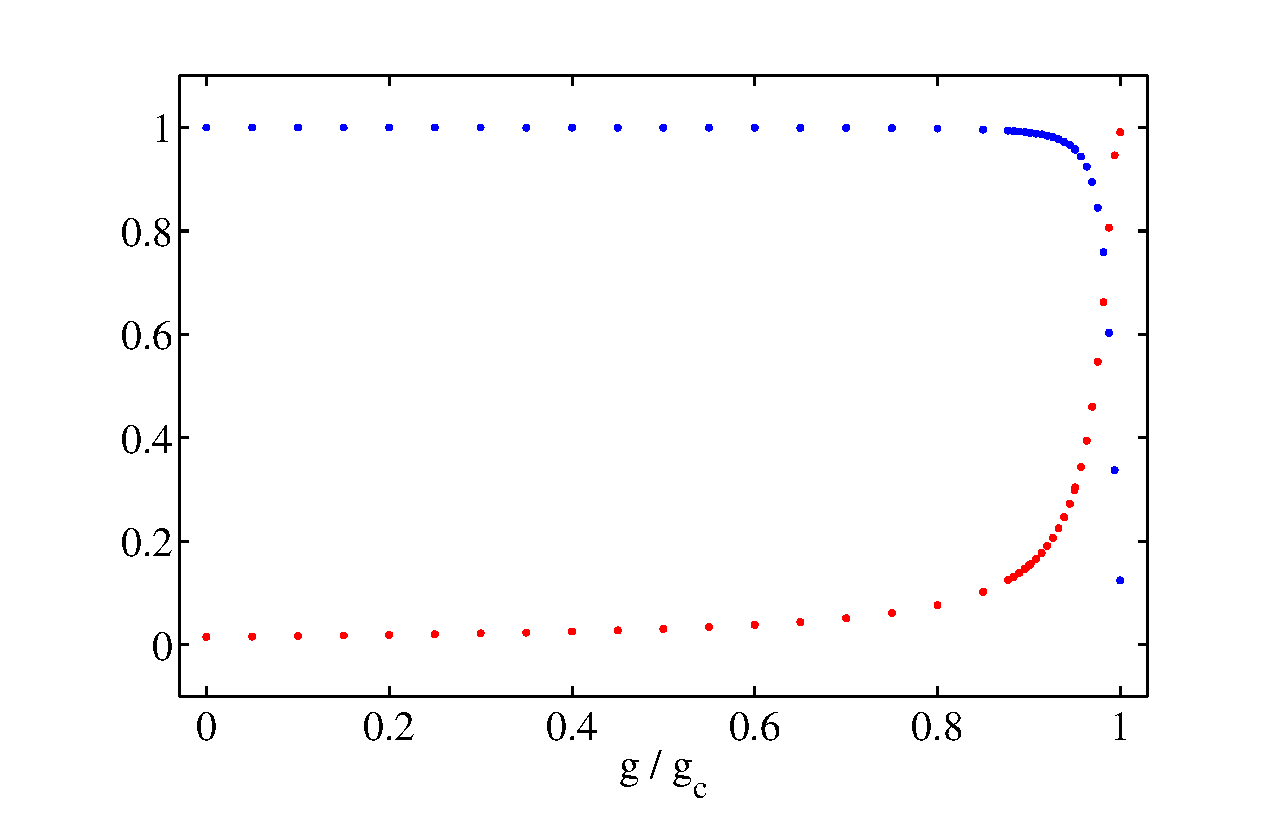
\includegraphics{pictures/alpha1_beta1}}}
%\scalebox{0.5}{\includegraphics{pictures/alpha_beta_reality_check}}}
\vskip -0.5cm
\caption[The left most plot is the electric field for a resonant frequency (blue shows a center of localization at $ \frac{1}{4} $L and is the LR orientation while red shows a center of localization at $ \frac{3}{4} $L and is the RL orientation.]{The left most plot is the electric field for a resonant frequency (blue shows a center of localization at $ \frac{1}{4} $L and is the LR orientation while red shows a center of localization at $ \frac{3}{4} $L and is the RL orientation. The other two plots are the alpha and beta coefficients scanning gain from  passive to critical gain at a resonant frequency for the two orientations. The center is LR and the right is RL. The crossover takes place very near critical gain. This explains why the amount of gain added is more sensitive near critical gain.}
\label{fig:alphabeta}
\end{figure}

What we get from these two plots in Fig.~\ref{fig:alphabeta} is that the two wave functions from the passive system are added up to get the wave form with gain, $ \tilde{\psi}$. The coefficients $\alpha$ and $\beta$ tell how much of each passive waveform to add. In the case of a wave function with center of localization at $ \frac{1}{4} $L there is hardly any contribution from the wave function with center of localization at $ \frac{3}{4} $L, so $\alpha$ and $\beta$ remain at their original 0 and 1 values. For the other canonical case $\alpha$ starts with hardly any contribution to $ \tilde{\psi}$ but as gain is added $\alpha$ dominates.

%%%%%%%%%%%%%%%%%%%%%%%%%%%%%%%%%%%%%%%%%%%%%%%%%%%%%%%%%
\subsection {Summary}
%%%%%%%%%%%%%%%%%%%%%%%%%%%%%%%%%%%%%%%%%%%%%%%%%%%%%%%%%

We were interested in finding a criteria for localization in media with gain.  We suspected the ratio of transmission and energy may be a good parameter.

The analytical diffusion model was the first thing we investigated.  Even though localization could not be present the diffusion equation demonstrated that T/${\cal E}$ was not divergent at the lasing threshold (even though transmission and energy both diverged). 

Next we created a computational model in Fortran for random layers of dielectric.  In this system there is no diffusion and localization does occur.  We used the transfer matrix method to propagate light using Maxwell's equations and recorded transmission, reflection, and electric field in the sample, (total energy in the sample).

Starting in the passive model we see that T/${\cal E}$ is neither smooth nor constant due to peaks in transmission that lack a corresponding peak in energy.  We then determined why this was occurring.  The electric field in the sample at that specific frequency lead us to show that localization is wave ``tunneling'' though the medium. We explain this by looking at two analytical models, the double barrier potential with varying well position and the periodic structure with a single defect. Now we know why there are peaks in transmission but not always energy. This explains why T/${\cal E}$ is not smooth.

Adding gain to the system makes T/${\cal E}$ smoother and it is a good parameter (in that it does not diverge) but T/${\cal E}$ is not constant due to the center of localization varying in the sample for different frequencies.

Flipping the sample and keeping the light that shines on the sample in the original orientation moves the center of localization to the opposite side. This is equivalent to keeping the sample fixed and flipping the light source orientation (now the light shines on the x=L side).

This change in boundary conditions (where the light is shined from) leads to insight on why the waveform of the electric field changes.  Reciprocity in the passive system allows us to construct two waveforms that constitute a basis, similar to the closed system and looking for eigenstates.  Adding gain to the system we use $\psi _1 $ and $\psi _2 $ as the basis.  We use coefficients $\alpha$ and $\beta$ to build the resultant waveform.

\begin{comment}

%%%%%%%%%%%%%%%%%%%%%%%%%%%%%%%%%%%%%%%%%%%%%%%%%%%%%%%%%
\subsection {Future work}
%%%%%%%%%%%%%%%%%%%%%%%%%%%%%%%%%%%%%%%%%%%%%%%%%%%%%%%%%

Now that we understand localization in systems with gain
we will go back and look at passive systems as a limit that
gain goes to zero.

We plan to investigate quasi 1-D systems,
then 2-D, and then 3-D. We should be able to verify that the
same ideas apply from the 1-D system.  Note that the 1-D potential
well extends easily to 2-D and 3-D, in that the boundary
conditions for the 1-D quantum mechanical potential well
are that the wave form is zero at the edges
of the well.

\end{comment}

\newpage
%\begin{appendices}
%%%%%%%%%%%%%%%%%%%%%%%%%%%%%%%%%%%%%%%%%%%%%%%%%%%%%%%%%
\subsection {Medium creation}
%%%%%%%%%%%%%%%%%%%%%%%%%%%%%%%%%%%%%%%%%%%%%%%%%%%%%%%%%
On first inspection, creating a media filled with random scatterers
seems a trivial task.  This is true for low density, as one simply
picks random positions and ensures that no two scatterers are too
close to each other.  However, localization occurs in high-density
scatterers.  There exists a maximum number of spheres that fits in a 
given volume, and as this upper limit is reach it becomes harder
to find the last available volumes to put the scattering sphere in.
For randomly positioned scatterers the upper limit is not well 
defined (realization specific), as the space between scatterers is not constant.

The initial algorithm implemented in code placed a scatterer in the medium by
choosing x,y,z from a uniformly random distribution. If the new position
conflicts with a previously choosen scatterer (distance between scatterers
is too small) then another choice of x,y,z is made. This process is repeated
until a valid scatterer position is found.  The number of unsuccessful 
choices grows with the number of total scatterers for a given volume as
$ ? $

To reduce this problem alternative algorithms were developed.

Instead of attempting to generate a random media, start with a 
lattice of scatterers and then let the scatterers take a random
walk.  However, this results on average that each scatterer is roughly
in the same place it started, a lattice.

Another option was to use a lattice and then allow the scattering
strength $\alpha$ to be random.  This is computationally simple but
introduces ?? band gap effects.

Breaking the medium into smaller containers

Stacking scatterers in the x direction. $\Delta x$ is not uniform, so
the distribution for choosing x,y,z was found.

\newpage
%\begin{appendices}
%%%%%%%%%%%%%%%%%%%%%%%%%%%%%%%%%%%%%%%%%%%%%%%%%%%%%%%%%
\subsection {propagation alternatives}
%%%%%%%%%%%%%%%%%%%%%%%%%%%%%%%%%%%%%%%%%%%%%%%%%%%%%%%%%
For 1D and quasi1D the incident light is a plane wave.  Using self-embedding
technique the eigen values numerical error in the transfer matrix was limited.
However, for certain parameters with quasi-1D the error prevented full investigation.

An alternative to plane wave is ray tracing, which introduces a different set
of complications. Instead of numerical inaccuracy, which can not be overcome, the 
difficulty is computational time. Individual photons are propagated through the 
medium, and a large number of photons is needed. There is error introduced in 
a discrete incident wave.  Even with a large number of incident photon paths, 
there exists the possibility of a path not being taken, since not all y-z choices 
are used.  Normally that would be acceptable, but localization demands that all 
paths be taken, less the one not taken results in the closed path.  By 
ignoring any path, we disregard a small number of localization occurrences.  
A finite number of incident photons ignores an infinite number of path possibilities.
The plane wave, continuous in y-z, takes all paths but error can build up in
the numerical accuracy of the transfer matrix eigenvalues.


\begin{comment}

useful sites for latex formatting
http://en.wikibooks.org/wiki/LaTeX/Mathematics
http://www.tex.ac.uk/cgi-bin/texfaq2html?label=appendix

********************************
conventions:

Fig.~\ref{fig:

Eq.~\ref{fig:

Ref.~\cite{

********************************

version history:

20080514
-changed energy from \xi to {\cal E}
-changed localization length from \zeta to \xi

20080506
-changed localization length \xi to \zeta
-added symbols appendix
-converted from pdf pictures to eps. Now run "latex" instead of "pdflatex"

20080421
-added hyperlinks
-changed energy E to \xi

\end{comment}




% model comparsion, tunneling
% T/E
%%20091214%%\section{quasi-1D}

\begin{comment}
 Outline:

Closed channels, renormalization of conductance *******************
0. Introduction
    a. motivation: why are closed channels important
    b. neglect them
1. Method
    a. numerical simulation model description
        i. generate random scatterer positions
        ii. free space and scatterer matrices multiplied
        iii. self-embedding technique
2. simulation results
    a. for N_c=0, model matches theory
    b. add N_c, there is a deviation in g.
        i. dependence on alpha, density
    c. with scaling, the N_c can be renormalized to N_c=0
        i. recovers lack of dependence on alpha, density
3. why it works
    a. folding technique description
        i. single scatterer
            -eliminate closed channels by matrix element renormalization
        ii. double scatterer
            -adds separation ("density") scaling
    b. supports conclusion on scattering strength alpha, density
4. conclusion
    a. review of main points
       -you can disregard N_c, as long as you do it correctly

Regimes plot development **********************
lengths
boundaries
explanation of regimes, characteristic behavior

Criterion for AL in active random media *****************
various passive criteria comparison


\end{comment}

In quasi-1D, the gain can be put in either the scatterers, the empty medium, or both. If one puts gain in the empty medium, then lasing can occur that is not due to localization (lasing due to boundary conditions of the waveguide). Since we are only interested in lasing due to strong localization, then the gain must be mathematically set in the scatterers. 


Note: our scattering potentials are based on $\delta$ functions, unlike the potentials developed in \cite{2007_Froufe-Perez_PRE} (in Appendix B).


Assume a rectangular metal waveguide with two dimensions, oriented such that the longer dimension is along the z-axis (length), and the shorter direction is the y-axis (width). The rectangular aspect ratio is such that there is no significant propagation along the y-axis (i.e. not two dimensional), but wide enough so that a scatterer does not cause only reflection (which would be one dimensional). Thus we define a quasi-1D waveguide between 1D and 2D. The motivation is to simplify a two-dimensional system using quantization of transverse momentum. This quasi-1D work scales to higher dimensions, unlike true one-dimensional models, which do not have closed channels. Two physical examples of quasi-1D systems are a mesoscopic metal wire and a disordered optical waveguide.

This model permits straightforward generalization to 3D waveguides. However, one would also need to consider the effect of polarization. %?Long-range mesoscopic correlations (?) of fields with different polarization (?)

our quasi-1D model  has the following adjustable parameters: $N_c$, $L$, $\alpha_s$, gain, $W$, $M$, $\omega$, sign of $\alpha_s$. These set the density and $N_o$. For output, we get directly $g$, ${\cal E}$, ${\cal E}^2$, $J_{pw}(z)$, $W_{pw}(z)$, $J_{uf}(z)$, $W_{uf}(z)$, $A(z)$, $B(z)$, $\hat{T}$, $\hat{R}$, correlation of energy(z). From these output, we can get $D(z)$, $\ell_{tmfp}$, $E(y,z)$. 

\subsection{assumptions and abstractions}
\glossary{name={model}, description={a mathematical abstraction of reality, for the purposes of capturing certain phenomena. As such, every model has limitations. }}

For a given model, assumptions must be enumerated.

% meta comment
%when can one be confident that the theoretical model is accurate? Only when the model accurately predicts experimental results

% meta comment
%Models are inherently non-physical because they seek generality. A model is only useful, though, if it captures the desired phenomena (and no extra phenomena). What are the limits of applicability for the models I use?

Specifically, a feature of the quasi-1D waveguide is the delta-function scatterers in free space. This simplifies the math by removing scattering physics, leaving transport physics.

choice of $\delta$-function scatterers has significant consequences:
\begin{itemize}
 \item easier to model mathematically (no spherical scattering math), while retaining the desired phenomenon: scattering from one channel to another
 \item inelastic scattering: no energy loss due to scattering when passive, and phase remains coherent [scatterers only affect amplitude].
 \item non-physical
 \item no saturation limit for number of closed channels
\end{itemize}

No noise is assumed (no spontaneous emission). This means that the transmission with gain will be slightly different compared to real output. Jon's model (from Yale) has noise (1D only).

The gain mechanism is purely mathematical: no atomic level modeling is included. This is part of being mesoscopic regime: independent of atomic conditions.

No input beam properties are assumed, other than the capability to be selectively incident on a specific channel.

By chosing planar quasi-1D geometry (and thus scalar waves), we implicitly assume that polarization will not significantly alter transport phenomena. Although planar geometry may be experimentally realizable, it is not as popular as 3D quasi-1D




\subsubsection{review of channels}

In a waveguide with two dimensions, the wave number $k = \frac{2 \pi}{\lambda} = \frac{\omega}{c}$ is broken into orthogonal components as $k^2 = k_{\parallel}^2 + k_{\bot}^2$. Solving for $k_{\parallel}$,
\begin{equation}
k_{\parallel} = \sqrt{k^2 - k_{\bot}^2}
\end{equation}
where $k_{\bot}$ is defined by the mode number of the sine function perpendicular to the direction of propagation, and is dependent on the waveguide width. %Due to boundary conditions imposed by the metallic (not leaky) waveguide, only wavefunctions that are zero at the boundary will propagate (sine functions in the y direction). Each sine function solution constitutes a ``channel.''
The two components are thus
\begin{equation}
 \begin{gathered}
  k_{\bot_n} =  \frac{n \pi}{W} \\
  k_{\parallel_n} = \sqrt{\left( \frac{2 \pi}{\lambda} \right)^2 - \left(\frac{n \pi}{W}\right)^2}
 \end{gathered}
\label{eq:wave_number_quasi1d}
\end{equation}
Note that for sufficient channel index, $k_{\parallel}$ becomes imaginary, denoted $i \kappa_{\parallel}$.  These channels, with an imaginary wave number, are the evanescent channels. The intensity decays exponentially because the exponent is real ($e^{i(i\kappa x)}$). 
% NOTE: Vellekoop's thesis says this is equivalent to spacial distribution (speckle) but gives no math


%%%%%%%%%%%%%%%%%%%%%%%%%%%%%%%%%%%%%%%%%%%%%%%%%%%%%%%%%%%%%%%%%%%%%%%%%%%%%%
\subsection {Introduction}
%%%%%%%%%%%%%%%%%%%%%%%%%%%%%%%%%%%%%%%%%%%%%%%%%%%%%%%%%%%%%%%%%%%%%%%%%%%%%%

In experimental studies of quasi-1D systems with randomly positioned 
scatterers there are open (propagating) channels and closed (evanescent)
channels.  
Dorokhov-Mello-Pereyra-Kumar (DMPK) theory 
%\cite{1988_Mello_Kumar_DMPK} 
%\cite{1982_Dorokhov_DMPK}
for quasi-1D geometry assumes
(1) all open channels are the same, and (2) closed channels can be disregarded.

Since the closed channels decay exponentially one normally
neglects these contributions in numerical simulations. If the detector is far way from the media
then the closed channels won't contribute. 

This is desirable, as the math is easier 
(which translates computationally to faster), and it is justified analytically
by calculations done for single scatterers~\cite{1990_Bagwell}~\cite{1991_Kumar_Bagwell}
and by rationalizing that if the density of scatterers is low enough, then 
there is sufficient separation between scatterers that closed channels do 
not contribute to interaction. However, since we are interested in Anderson 
localization, we will be in the high density, low scattering strength regime.
In this regime it would appear that we can not ignore the effect
of closed channels.  Then the ability to numerically model systems becomes
questionable since real systems have an infinite number of closed channels.

A numerical simulation is described that models an arbitrary number of point scatterers
in a quasi-1D waveguide where each has the same scattering strength. 
We can vary the number of open and closed channels,
scattering strength, system dimensions, and scatterer density. 
The significance of closed modes can be studied through 
numerical simulation to determine how a finite number of these modes 
affect the wave propagation through the random medium.  In a real 
system there are an infinite number of closed channels.  It is
shown that closed channels can be ignored, which is useful as accounting for an infinite
number is difficult or impossible.
Using this computational model we verify theoretical concepts. Self-embedding 
technique
%~\cite{1999_yamilov_selfembed}
~\cite{1976_Bellman_Wing_embedding}
extends the limits of numerical simulation when closed channels are added, but this
does not allow for an arbitrary number of closed channels as numerical inaccuracy
still emerges.

The scattering matrices for one scatterer and two scatterers are also
derived. We show that folding the closed channels is both possible, and in numerical 
simulation, necessary.  

This work applies to higher dimensions in that it scales, unlike one-dimensional
models which do not have closed channels. Physical examples of quasi-1D systems 
are mesoscopic metal wire and disordered optical waveguide.

Conductance g is observed to be uniform, even if contribution of the channels
are non-uniform [need more here]. 

\begin{equation}
g = \sum_a \sum_b T_{a,b}
% See Ben's notes, 20080610
\end{equation}

Scattering length as a function of three parameters, density, scattering strength, and number of closed, or 
evanescent, channels is determined. (?)

Quantization of transverse momentum allows for the simplification of 
this two-dimensional system to a one-dimensional system referred to as 
quasi-1D. This model permits straightforward generalization to 3D waveguides, 
in which one would need to consider the effect of polarization, such as long-range mesoscopic 
correlations (?) of fields with different polarization.

%%%%%%%%%%%%%%%%%%%%%%%%%%%%%%%%%%%%%%%%%%%%%%%%%%%%%%%%%%%%%%%%%%%%%%%%%%%%%%
\subsubsection {Numerical Simulation Model Description}
%%%%%%%%%%%%%%%%%%%%%%%%%%%%%%%%%%%%%%%%%%%%%%%%%%%%%%%%%%%%%%%%%%%%%%%%%%%%%%

Evolution of electric field through the system is 
described with a set of transfer matrices in terms of open and closed channels
of the waveguide.  This ensures the continuity of both the electric field 
and its derivative throughout the waveguide.  Parameters such as the length
and width of the waveguide, the number of open and closed channels (real 
and evanescent modes), the number of scatterers, and the scattering strength
of scatterers determine how the light will propagate through the 
waveguide. The wave vector k for both open and closed channels is calculated,
n being the mode number, W the width, c speed of light in a vacuum.

\begin{equation}
\begin{gathered}
k_{\perp n}=n\pi /W \\
k_{\parallel n}=\sqrt{(w/c)^2-k_{\perp n}^2}
\end{gathered}
\label{kwaveguide}
\end{equation}

The wavelength is normalized to one for all simulations.  
% Maybe not?: 
%[wavelength] lambda * [frequency] f = [angular frequency] omega / [wavenumber] k
Each channel, open and closed, has both a perpendicular and parallel wave vector components.
From Equ.~\ref{kwaveguide} if $K_{\parallel n}$ is real the channel is open, $K_{\parallel n}$ imaginary 
corresponds to closed.  The total number of channels ($N_{max}$) is
studied systematically to determine the effects of closed channels and 
includes the open channels.

Wave propagation is described as follows.  The values for the electric 
field and its derivative are stored for each mode at each layer, scatterer 
or free space, in matrices. The electric field and its derivative for free 
space propagation of open channels are given by:

\begin{equation}
\begin{gathered}
E_n(x+\Delta x)=E_n(x)cos(K_{\parallel n}\Delta x)+K_{\parallel n}^{-1}
E_n^{'}(x)sin(K_{\parallel n}\Delta x) \\
K_{\parallel n}^{-1}E_n^{'}(x+\Delta x)=-E_n(x)sin(K_{\parallel n} \Delta x)
+K_{\parallel n}^{-1}E_n^{'}(x)cos(K_{\parallel n}\Delta x)
\end{gathered}
\label{electricfield}
\end{equation}

For the closed channels, the field equations are the similar to 
Equ.~\ref{electricfield} except $K$ is replaced by the imaginary $\kappa$.

\begin{comment}
%% REDUNDANT
\begin{equation}
\begin{gathered}
E_n(x+\Delta x)=E_n(x)cosh(\kappa_{\parallel n}\Delta x)+
\kappa_{\parallel n}^{-1}E_n^{'}(x)sinh(\kappa_{\parallel n}\Delta x)\\
\kappa_{\parallel n}^{-1}E_n^{'}(x+\Delta x)=E_n(x)sinh(\kappa_{\parallel n}
\Delta x)+\kappa_{\parallel n}^{-1}E_n^{'}(x)cos(\kappa_{\parallel n}\Delta x)
\end{gathered}
\end{equation}
\end{comment}

The electric field after each scattering event must be equal to the
initial field, where the first derivative is given by:

\begin{equation}
\begin{gathered}
E_n(x+\Delta x)=E_n(x)\\
E_n^{'}(x+\Delta x)=E_n^{'}(x)-\alpha(\frac{\omega}{c})^2\sum_{m=1}^{n_{max}}
A_{nm}E_m(x) 
\end{gathered}
\end{equation}

and

\begin{equation}
A_{nm}=\frac{2}{W}sin(K_{\perp n}y)sin(K_{\perp m}y)
\end{equation}
\begin{equation}
K_{\parallel n}=i\kappa_{\parallel n}
\end{equation}

Alpha describes the scattering strength of the scatterers. Thus wave
propagation can be described by $2 N_{max} x 2 N_{max}$ matrices of two types:
propagation or free space matrices, and scattering matrices. 
See Fig.~\ref{fig:tomsmatrices}

\begin{figure}
\vskip -0.5cm
\centerline{
\scalebox{1}{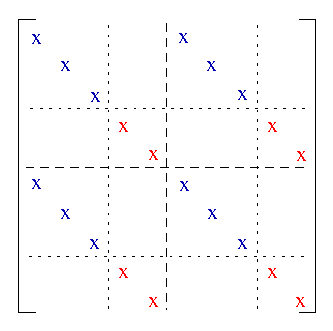
\includegraphics{pictures/propagation_matrix}}
\quad \quad \quad \quad
\scalebox{1}{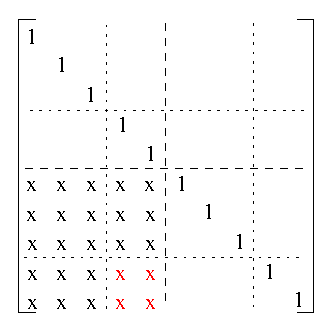
\includegraphics{pictures/scattering_matrix}}}
\vskip -0.5cm
\caption{Propagation or Free Space Matrices (left),
and Scattering Matrices (right). ``x'' denotes non-zero terms, which are not necessarily the same. 
Each matrix is separated into four $N_{max} x N_{max}$ quadrants 
(long dashed portions), each containing information from open channels
(upper left short dashed portions) as well as closed (lower right short
dashed portions). }
\label{fig:tomsmatrices}
\end{figure}

These matrices are combined to form a total matrix.
This matrix contains the propagation of the CW electric field information through the 
waveguide. The total matrix is used to calculate the reflection and
transmission coefficients for each mode.

%%%%%%%%%%%%%%%%%%%%%%%%%%%%%%%%%%%%%%%%%%%%%%%%%%%%%%%%%%%%%%%%%%%%%%%%%%%%%%
\subsubsection {Self-Embedding}
%%%%%%%%%%%%%%%%%%%%%%%%%%%%%%%%%%%%%%%%%%%%%%%%%%%%%%%%%%%%%%%%%%%%%%%%%%%%%%

Due to the numerical instability which builds up in longer disordered
waveguides, the computation of the simple product of individual matrices is
not sufficient, as the eignvalues become divergent. The self-embedding method is introduced 
slow the growth of computational error inherent in numerical matrix multiplication.
This method consistently corrects any deviation caused by rounding on every step of the multiplication and 
gives increased accuracy to the final result.  % I don't think this is correct; it just prolongs the time until matrices become unstable (determinant not equal to 1)

Start with the vector describing $N$ open and $N_c$ closed channels for both
the electric field and the field derivative, total length $N+N_c+N+N_c$, on the
incident side of the medium: $\vec{v}(0)$.  There is a similar vector on the otherside
of the quasi-1D waveguide, $\vec{v}(L)$, of the same dimension. For $\vec{v}(0)$, assume a an
input beam in one channel, $n_0$. (Later on the input channel will be iterated over
all open channels. The input could be to closed channels, but that is not investigated
in this letter.)

Given $\vec{v}(0)$ and $\vec{v}(L)$ a pair of matrices is sought that satisfies
\begin{equation}
\hat{G}\vec{v}(0) + \hat{H}\vec{v}(L) = \vec{v}_{BC}
\label{selfEmbedGHvBC}
\end{equation}
such that $\vec{v}_{BC}$ has no dependence on variables, transmission, or reflection.
Any $\hat{G}$ and $\hat{H}$ that satisfies these conditions can be used. We use
Fig.~\ref{fig:HGmatrix} which results in $\vec{v}_{BC}$ having zeros in all elements
except for the input channel, where there is a ``2''.  

Now that $\hat{G}$ and $\hat{H}$ are set, S is

\begin{equation}
\hat{S} = (\hat{H} + \hat{G})^{-1}
\label{selfEmbedSinvGH}
\end{equation}



Self-embedding uses inverses, which add to computational time.


%~\cite{1999_yamilov_selfembed}
%~\cite{1976_Bellman_Wing_embedding}

\begin{figure}
\vskip -0.5cm
\centerline{
\scalebox{1}{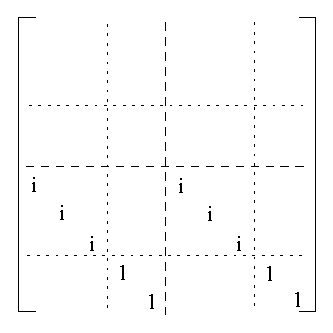
\includegraphics{pictures/H_matrix}}
\quad \quad \quad \quad
\scalebox{1}{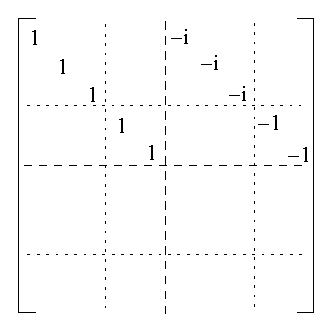
\includegraphics{pictures/G_matrix}}}
\vskip -0.5cm
\caption{Boundary conditions (?). H on left, G on right.}
\label{fig:HGmatrix}
\end{figure}

Transmission and reflection vectors are related to the S matrix
(part of the total matrix(?)) that is determined via the self-embedding procedure:

Each time the simulation self-embeds multiple matrix inversions must
be calculated (?).  These calculations take longer than a simple matrix
multiplication, but the method prevents the buildup of numerical
error (describe this more).  More self-embedding loops means a longer simulation run time.

Even with self-embedding technique, the number of closed channels is computationally limited.
The numerical limits depend on scattering density, system length (number of transfer matrices).

%%%%%%%%%%%%%%%%%%%%%%%%%%%%%%%%%%%%%%%%%%%%%%%%%%%%%%%%%%%%%%%%%%%%%%%%%%%%%%
\subsection {Numerical simulation results}
%%%%%%%%%%%%%%%%%%%%%%%%%%%%%%%%%%%%%%%%%%%%%%%%%%%%%%%%%%%%%%%%%%%%%%%%%%%%%%
%
%outline:
%    a. for N_c=0, model matches theory
%    b. add N_c, there is a deviation in g.
%        i. dependence on alpha, density
%    c. with scaling, the N_c can be renoralized to N_c=0
%        i. recovers lack of dependence on alpha, density

This table shows the preliminary results of the scattering lengths
obtained using this method.  The scattering lengths describe the rate at which
the energy is removed from the input channel.  It is a function of two
parameters, the scattering density and the strength of the individual
scatterer.  The results displayed on the following page show, as expected,
the scattering lengths decrease as the scattering strength increases.  This is
also the trend for density.

\begin{figure}
\vskip -0.5cm
\centerline{
\scalebox{.5}{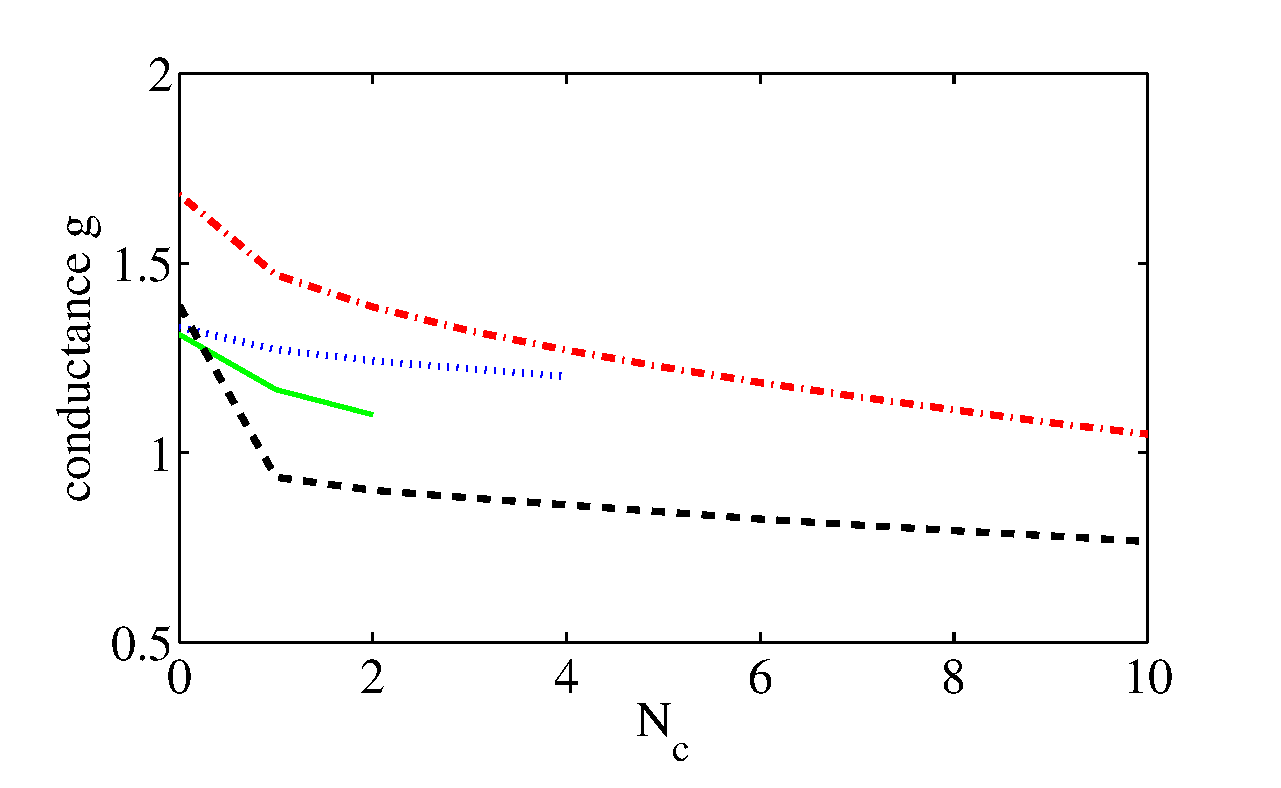
\includegraphics{pictures/conductivity_g_versus_N_closed}}}
\vskip -0.5cm
\caption{conductance versus number of closed channels $N_c$ for varying
scattering strength and density. (Which is which?) Dotted blue is, solid
green is, dot-dashed red is, and dashed black is .}
\label{fig:gVersusNc}
\end{figure}
  %Supporting charts or tables that demonstrate the scattering length
  %dependence on density and alpha

The figures above illustrate the transition which occurs in the transmission
matrix ($T_{ab}$) as the length of the sample increases for a fixed density and
scattering strength.  A is the input channel number (Horizontal axis) and B is
the output channel number (Vertical axis).  One can see initially that the
shortest sample (left) only the diagonal components of not equal to zero.
This corresponds to the wave emerging from the same channel as it was launched
into.  One can see from the right panel, for a very long system, the light
emerges in all output channels.

\begin{figure}
\vskip -0.5cm
\centerline{
\scalebox{.3}{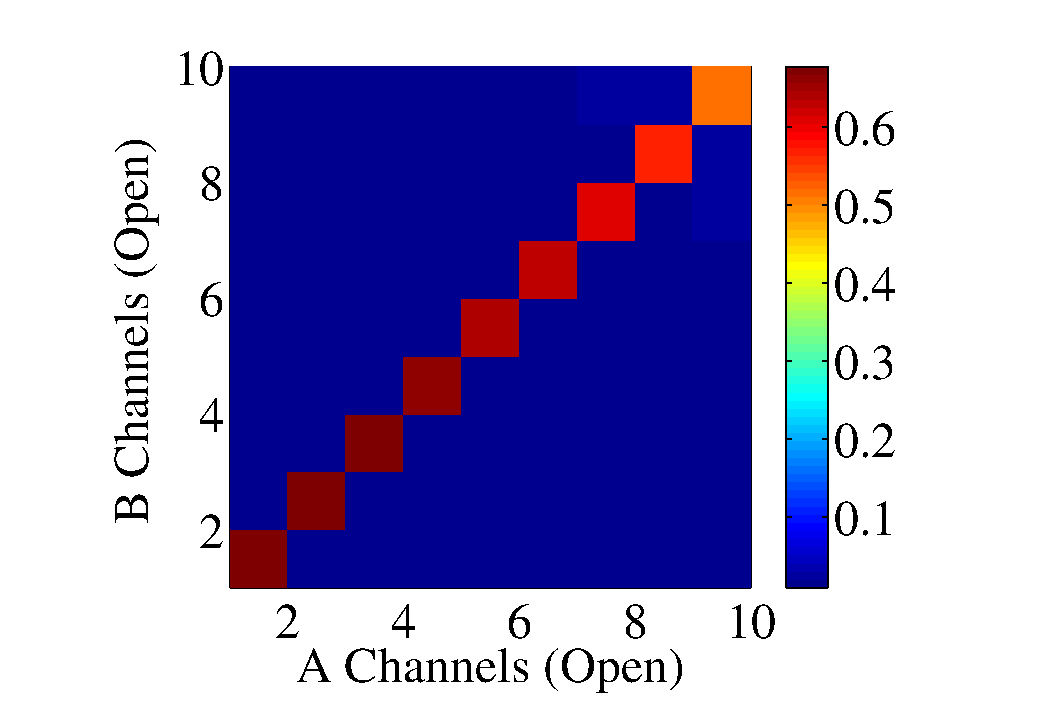
\includegraphics{pictures/low_scattering}}
\scalebox{.3}{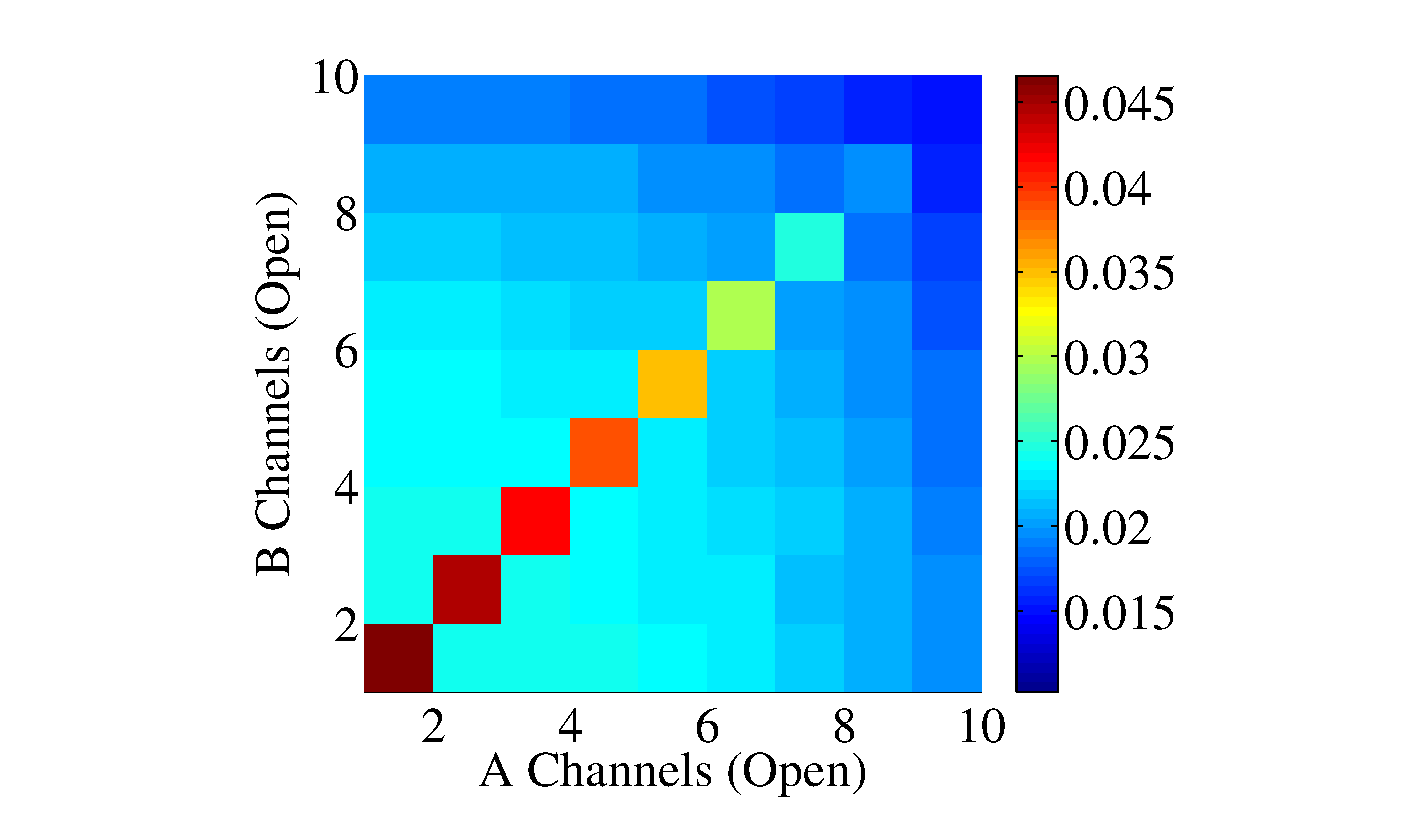
\includegraphics{pictures/mid_scattering}}
\scalebox{.25}{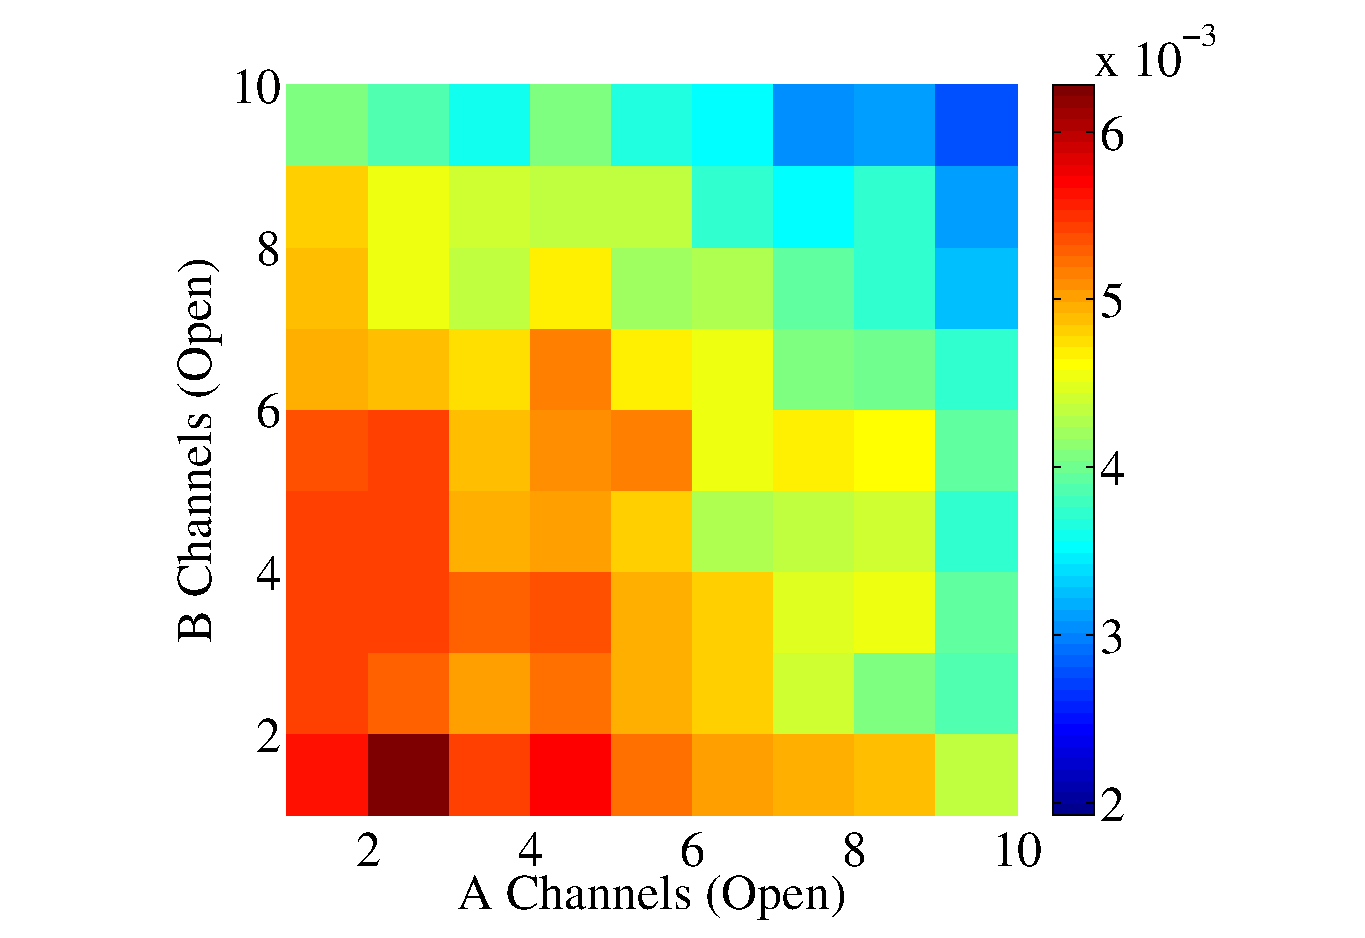
\includegraphics{pictures/high_scattering}}}
\vskip -0.5cm
\caption{Matrices describing scattering from an input channel to an output channel
for 10 open channels; arbitrary units?  Left: for few scattering events in the 
medium it is likely that light will not scattering into a different channel. Even
at low scattering probability the channels are not uniform (higher concentration
of (?) in lower channel numbers). As the scattering event probability is increased
(higher scatterer density or longer system length), inter-channel scattering is 
observed.  At high scattering density (?)}
\label{fig:channelMatrices}
\end{figure}


The model suggests that saturation (a finite number of closed 
channels) is attainable given that the parameters fit a constraint:
\begin{equation}
(m / (\hbar^2 \kappa _n))(\lambda/W) <<1
\end{equation}
% page 358 of \cite{1990_Bagwell}



%%%%%%%%%%%%%%%%%%%%%%%%%%%%%%%%%%%%%%%%%%%%%%%%%%%%%%%%%%%%%%%%%%%%%%%%%%%%%%
\subsection {Why closed channels can be renormalized: Quasi-1D theoretical models}
%%%%%%%%%%%%%%%%%%%%%%%%%%%%%%%%%%%%%%%%%%%%%%%%%%%%%%%%%%%%%%%%%%%%%%%%%%%%%%
%    a. folding technique description
%        i. single scatterer
%            -eliminate closed channels by matrix element renormalization
%        ii. double scatterer
%            -adds seperation ("density") scaling
%    b. supports conclusion on scattering strength alpha, density

In order to model quasi-1D system with random defects one must know how to 
deal with a single defect. It is then assumed that additional defects can be
extrapolated. The math for a single defect in a waveguide can be dealt with 
using transfer matrices or Greene's functions %~\cite{??}.

A matrix that describes open and closed channels is of size $(N+N_c)x(N+N_c)$
where $N$ is the number of open channels, $N_c$ is the number of closed channels.
We derive in appendix A how to reduce matrices of rank $N_c$ to rank $N$,
called folding, as the closed channels are incorperated into the open channels.
There is a conservation of information, in that the information stored in the original
$(N+N_c)x(N+N_c)$ matrix is still contained within the new ``folded'' $NxN$
matrix, albeit messier elements.  Although messier, by
induction (using the developed recursion relation) it has been demonstrated that 
an $NxN$ matrix can account for N open channels and an infinite number of closed channels $N_c$.  The math
done is a correction to ~\cite{1990_Bagwell} and is a more explicit reworking of~\cite{1991_Kumar_Bagwell}.

With a single scatterer model scattering strength can be modeled, 
but the separation between two scatterers is not present. Thus if 
there are many scatterers the effect of density on scattering length can not
be accounted for by a single scatterer. In order to model interaction of 
scatters by both the open and closed channels, one needs to derive the math
for at minimum two scatterers, as is done in %~\cite{??}.

%%%%%%%%%%%%%%%%%%%%%%%%%%%%%%%%%%%%%%%%%%%%%%%%%%%%%%%%%%%%%%%%%%%%%%%%%%%%%%
\subsection {Conclusion}
%%%%%%%%%%%%%%%%%%%%%%%%%%%%%%%%%%%%%%%%%%%%%%%%%%%%%%%%%%%%%%%%%%%%%%%%%%%%%%
% outline:
% i structure of the model
% divergence of closed channels
% Nc is important to include but hard to model (due to divergence)
% conclusion: can ignore Nc, but need to renormalize mean free path
% include a discussion of self-embedding
% why self-embedding necessary:
% 	exponential behavior of closed channels
% 	open and closed channels cause divergence in matrices
% 	 -> self-embedding renormalizes the matrices and reduces the divergence

Using a numerical simulation of a quasi-1D waveguide with densely packed
randomly placed scatterers the effect of closed channels on was investigated.
Using transfer matrices, open and closed channels are varied.  The number of
matrices multiplied is limited by numerical accuracy, and is extended using self-embedding technique.

However, even with a perfect numerical simulation the effect of closed channels
can not be accounted for, as (?) does not reach an asymptote.

Thus analytically folding the closed channels is necessary.  The effect on 
numerical simulations is acceptable by renormalizing conductance.

Verified that the numerical model, analytical single scatterer, and 
analytical two scatterer results match.


Increasing $N_c$ is effectively the same as increasing system Length. Thus we can 
disregard $N_c$ (?) Or maybe this is a way to account for it?

The folding (in the appendix) shows that one can disregard $N_c$ by using a 
different NxN matrix


% closed channels
% regimes plot
% criteria
%%20091214%%\section{3D waveguide}

I'll call this system quasi-1D cubic, to avoid confusion



\subsection{applictions}
%%20091214%%%\begin{center}SECTION\end{center}

\chapter{CONCLUSIONS}

\section{CHARACTERIZATION OF TRANSPORT REGIME TRANSITIONS IN NON-CONSERVATIVE RANDOM MEDIA}

The purpose of the first portion of this dissertation was to characterize the effect of absorption and gain in ballistic, diffusive, and localized transport regimes. Particle and wave-based transport models were studied in one dimension (1D) and quasi-1D geometries. 

An investigation of the ratio of transmission to energy in the system, $T/{\cal E}$, was performed in 1D using theoretical and numerical methods~\cite{2010_Payne_TE}. %~(c.f.~Section \ref{sec:TE2009}). 
The numerical model uses the transfer matrix method~\cite{1981_MacKinnon_scaling} with self-embedding~\cite{1999_yamilov_selfembed} to simulate layers of dielectric material with random widths. Since diffusion cannot occur in 1D, the response of the parameter $T/{\cal E}$ in the regime of Anderson localization when gain is present was found. A decrease of $T/{\cal E}$ from the value given by the classical un-renormalized diffusion coefficient may be attributed to wave-interference localization effects. Although $T/{\cal E}$ does not diverge as the random lasing threshold is approached, there is a dependence on the position of the center of localization. This position dependence is closely related to the existance of necklace states~\cite{1987_Pendry}. 

To investigate the transition from diffusion to Anderson localization, the previous numerical model was extended to quasi-1D geometry. To guide our efforts we developed a phase space diagram with 15 different transport regimes~\cite{2010_Yamilov_Regimes}. A way of characterizing which regime a given system is in was clearly needed. In the process of using the numerical model in this geometry, we showed that evanescant channels do not need to be included in simulations of passive media~\cite{2010_Payne_closed}. The effect of evanescant channels is renormalize the transport mean free path while conforming to single parameter scaling. 

A parameter related to $T/{\cal E}$, the position dependent diffusion coefficient $D(z)$, was investigated for use in characterizing the multiple transport regimes in quasi-1D non-conservative random media~\cite{2010_Payne_PRL}. Our results indicate that $D(z)$ may serve as a useful criterion for the enumerated transport regimes. 

\section{ANALYSIS OF DETERMINISTIC APERIODIC STRUCTURES}



Although random media produces novel features, these systems lack easy reproducibility. For applications such as photonic integrated circuits we are interested in novel features unavailable to periodic media while maintaining reproducibility. Thus media correlated disorder is a natural avenue of pursuit. The numerical model used in this dissertation can simulate any arrangement of scatters, making it amenable to aperiodic media. %The same simulation tool used for random media was applied to aperiodic media. 

In the studies of deterministic aperiodic structures (DAS) we focused on the Thue-Morse pattern. This generation algorithm yeilds a singular continuous Fourier transform spectrum with self-similar features. We demonstrated the possibility of mapping the array of micro-cavities in the two dimensional (2D) Thue Morse DAS onto a periodic square lattice~\cite{2012_Payne_Mapping_2D_TM}. Such mapping allowed us to uniquely identify and enumerate the configurations of nearest and next-nearest neighbors. Thus the original aperiodic structure is reduced to the periodic structure with aperiodic arrangement of the limited set of pairings. 

Once this step was completed, we demonstrated the applicability of the tight binding approach in a deterministic aperiodic array of photonic micro-cavities. Under realistic conditions, we observed hybridization of the modes of individual micro-cavities into the eigenstates of the entire array. Our work adds the tight binding approach to the arsenal of theoretical tools for studying of 2D~Thue-Morse structures as well as for design and analysis of experiments.

The tight binding model allows us to investigate the size scaling of the density of the optical states in large arrays of optical micro-cavities; monitor the evolution of the spectra; and to study spatial properties of the eigenstates via e.g. the inverse participation ratio. The inverse participation ratio shows coexistence of localized and extended states in the same spectral regions. Some of the extended states have nearly constant intensity across the entire sample. This property makes the considered system extremely promising for practical applications in optical control of light propagation via e.g. wave-front shaping.
 


%\section{TEST OF BORDERS}

%Lorem ipsum dolor sit amet, consectetuer adipiscing elit. Ut purus elit, vestibulum ut, placerat ac, adipiscing vitae, felis. Curabitur dictum gravida mauris. Nam arcu libero, nonummy eget, consectetuer id, vulputate a, magna. Donec vehicula augue eu neque. Pellentesque habitant morbi tristique senectus et netus et malesuada fames ac turpis egestas. Mauris ut leo. Cras viverra metus rhoncus sem. Nulla et lectus vestibulum urna fringilla ultrices. Phasellus eu tellus sit amet tortor gravida placerat. Integer sapien est, iaculis in, pretium quis, viverra ac, nunc. Praesent eget sem vel leo ultrices bibendum. Aenean faucibus. Morbi dolor nulla, malesuada eu, pulvinar at, mollis ac, nulla. Curabitur auctor semper nulla. Donec varius orci eget risus. Duis nibh mi, congue eu, accumsan eleifend, sagittis quis, diam. Duis eget orci sit amet orci dignissim rutrum. Nam dui ligula, fringilla a, euismod sodales, sollicitudin vel, wisi. Morbi auctor lorem non justo. Nam lacus libero, pretium at, lobortis vitae, ultricies et, tellus. Donec aliquet, tortor sed accumsan bibendum, erat ligula aliquet magna, vitae ornare odio metus a mi. Morbi ac orci et nisl hendrerit mollis. Suspendisse ut massa. Cras nec ante. Pellentesque a nulla. Cum sociis natoque penatibus et magnis dis par turient montes, nascetur ridiculus mus. Aliquam tincidunt urna. Nulla ullamcorper vestibulum turpis. Pellentesque cursus luctus mauris. Lorem ipsum dolor sit amet, consectetuer adipiscing elit. Ut purus elit, vestibulum ut, placerat ac, adipiscing vitae, felis. Curabitur dictum gravida mauris. Nam arcu libero, nonummy eget, consectetuer id, vulputate a, magna. Donec vehicula augue eu neque. Pellentesque habitant morbi tristique senectus et netus et malesuada fames ac turpis egestas. Mauris ut leo. Cras viverra metus rhoncus sem. Nulla et lectus vestibulum urna fringilla ultrices. Phasellus eu tellus sit amet tortor gravida placerat. Integer sapien est, iaculis in, pretium quis, viverra ac, nunc. Praesent eget sem vel leo ultrices bibendum. Aenean faucibus. Morbi dolor nulla, malesuada eu, pulvinar at, mollis ac, nulla. Curabitur auctor semper nulla. Donec varius orci eget risus. Duis nibh mi, congue eu, accumsan eleifend, sagittis quis, diam. Duis eget orci sit amet orci dignissim rutrum. Nam dui ligula, fringilla a, euismod sodales, sollicitudin vel, wisi. Morbi auctor lorem non justo. Nam lacus libero, pretium at, lobortis vitae, ultricies et, tellus. Donec aliquet, tortor sed accumsan bibendum, erat ligula aliquet magna, vitae ornare odio metus a mi. Morbi ac orci et nisl hendrerit mollis. Suspendisse ut massa. Cras nec ante. Pellentesque a nulla. Cum sociis natoque penatibus et magnis dis par turient montes, nascetur ridiculus mus. Aliquam tincidunt urna. Nulla ullamcorper vestibulum turpis. Pellentesque cursus luctus mauris. Lorem ipsum dolor sit amet, consectetuer adipiscing elit. Ut purus elit, vestibulum ut, placerat ac, adipiscing vitae, felis. Curabitur dictum gravida mauris. Nam arcu libero, nonummy eget, consectetuer id, vulputate a, magna. Donec vehicula augue eu neque. Pellentesque habitant morbi tristique senectus et netus et malesuada fames ac turpis egestas. Mauris ut leo. Cras viverra metus rhoncus sem. Nulla et lectus vestibulum urna fringilla ultrices. Phasellus eu tellus sit amet tortor gravida placerat. Integer sapien est, iaculis in, pretium quis, viverra ac, nunc. Praesent eget sem vel leo ultrices bibendum. Aenean faucibus. Morbi dolor nulla, malesuada eu, pulvinar at, mollis ac, nulla. Curabitur auctor semper nulla. Donec varius orci eget risus. Duis nibh mi, congue eu, accumsan eleifend, sagittis quis, diam. Duis eget orci sit amet orci dignissim rutrum. Nam dui ligula, fringilla a, euismod sodales, sollicitudin vel, wisi. Morbi auctor lorem non justo. Nam lacus libero, pretium at, lobortis vitae, ultricies et, tellus. Donec aliquet, tortor sed accumsan bibendum, erat ligula aliquet magna, vitae ornare odio metus a mi. Morbi ac orci et nisl hendrerit mollis. Suspendisse ut massa. Cras nec ante. Pellentesque a nulla. Cum sociis natoque penatibus et magnis dis par turient montes, nascetur ridiculus mus. Aliquam tincidunt urna. Nulla ullamcorper vestibulum turpis. Pellentesque cursus luctus mauris. Lorem ipsum dolor sit amet, consectetuer adipiscing elit. Ut purus elit, vestibulum ut, placerat ac, adipiscing vitae, felis. Curabitur dictum gravida mauris. Nam arcu libero, nonummy eget, consectetuer id, vulputate a, magna. Donec vehicula augue eu neque. Pellentesque habitant morbi tristique senectus et netus et malesuada fames ac turpis egestas. Mauris ut leo. Cras viverra metus rhoncus sem. Nulla et lectus vestibulum urna fringilla ultrices. Phasellus eu tellus sit amet tortor gravida placerat. Integer sapien est, iaculis in, pretium quis, viverra ac, nunc. Praesent eget sem vel leo ultrices bibendum. Aenean faucibus. Morbi dolor nulla, malesuada eu, pulvinar at, mollis ac, nulla. Curabitur auctor semper nulla. Donec varius orci eget risus. Duis nibh mi, congue eu, accumsan eleifend, sagittis quis, diam. Duis eget orci sit amet orci dignissim rutrum. Nam dui ligula, fringilla a, euismod sodales, sollicitudin vel, wisi. Morbi auctor lorem non justo. Nam lacus libero, pretium at, lobortis vitae, ultricies et, tellus. Donec aliquet, tortor sed accumsan bibendum, erat ligula aliquet magna, vitae ornare odio metus a mi. Morbi ac orci et nisl hendrerit mollis. Suspendisse ut massa. Cras nec ante. Pellentesque a nulla. Cum sociis natoque penatibus et magnis dis par turient montes, nascetur ridiculus mus. Aliquam tincidunt urna. Nulla ullamcorper vestibulum turpis. Pellentesque cursus luctus mauris.



% Leave the following two lines alone:
\appendix            % This command is used only once!
                     % It resets the formatting for the appendices.
%\let\cleardoublepage\clearpage
%%20091214%%\section{layman's overview}

The minimum to understand Anderson Localization is the concept of wave interference. 

useful mathematical concepts: linear algebra, calculus, partial differential equations

-Emergence: whole is different from the sum of its parts
   -diffusion, localization can not be seen from the perspective of inter-molecular interactions.

localization, diffusion are processes that arise from multiple events. What's the minimum number of events to constitute diffusion, localization?  
-how many people constitute a society? 
-how many atoms needed to demonstrate a phase change?

Answer: as many samples as are needed to get ensemble behavior, such that adding more samples does not affect the distribution.

This is an important question computationally, as you want to be able to claim universal behavior using ensemble averages, but you want to be doing the minimum number of samples required.  For example, 100,000 realizations to yield 0.000001 accuracy. Another example, $L=5 \lambda$
%%20091214%%\section{1D transfer matrix and A,B}
We derive the transfer matrix for a 1D dielectric layer of length $a_1$ and index of refraction $n_1$. The block of material ``1'' is adjacent to another block ``0'' which contains the incident wave. The boundary conditions at each layer edge are that the electric field and the derivative match.
\begin{equation}
\begin{gathered}
E_o = E_1\\
\frac{dE_o}{dx} = \frac{dE_1}{dx}
\end{gathered}
\end{equation}
The general wave function $E=A \exp(-i k n x) + B \exp(i k n x)$ and its derivative must match coefficents: $A_o, B_o$ at $x=0$ with $A_1, B_1$ at $x=a_1$.
\begin{equation}
\begin{gathered}
A_o + B_o = A_1 \exp(-i k n_1 a_1) + B_1 \exp(i k n_1 a_1)\\
i k n_o (A_o - B_o) = i k n_1 (A_1 \exp(-i k n_1 a_1) - B_1 \exp(i k n_1 a_1))
\end{gathered}
\label{eq:match_field_deriv}
\end{equation}
The goal is to solve for $A_1$,$B_1$ in terms of $A_0$,$B_0$ and get the general form
\begin{equation}
\begin{gathered}
A_1 = A_o T_{11} + B_o T_{12} \\
B_1 = A_o T_{21} + B_o T_{22}
\end{gathered}
\end{equation}
The matrix $T$ will be the transfer of field from $A_0$,$B_0$ to $A_1$,$B_1$. First, rewrite Eq.~\ref{eq:match_field_deriv} as
\begin{equation}
\begin{gathered}
(A_o + B_o) \exp(-i k n_1 a_1) = A_1 \exp(-2 i k n_1 a_1) + B_1 \\
i k n_o (A_o - B_o) \exp(-i k n_1 a_1) = A_1 \exp(-2 i k n_1 a_1) - B_1
\label{fig:terms}
\end{gathered}
\end{equation}
Then Eq.~\ref{fig:terms} sums to
\begin{equation}
(A_o + B_o) \exp(-i k n_1 a_1) + \frac{i k n_o}{i k n_1} (A_o - B_o) \exp(-i k n_1 a_1) = 2 A_1 \exp(-2 i k n_1 a_1)
\end{equation}
Solve for $A_1$ in terms of $A_o$ and $B_o$. The coefficents of $A_o$ and $B_o$ are $T_{11}$ and $T_{12}$.
\begin{equation}
\begin{gathered}
T_{11} = \frac{1}{2} (1 + \frac{n_o}{n_1} ) \exp(i k n_1 a_1) \\
T_{12} = \frac{1}{2} (1 - \frac{n_o}{n_1} ) \exp(i k n_1 a_1)
\end{gathered}
\end{equation}
Similarly, solve for $B_1$ in terms of $A_o$ and $B_o$. The coefficents of $A_o$ and $B_o$ are $T_{21}$ and $T_{22}$.
\begin{equation}
\begin{gathered}
T_{21} = \frac{1}{2} (1 - \frac{n_o}{n_1} ) \exp(-i k n_1 a_1) \\
T_{22} = \frac{1}{2} (1 + \frac{n_o}{n_1} ) \exp(-i k n_1 a_1)
\end{gathered}
\end{equation}
These are the matrix elements for the transfer matrix.
\begin{equation}
T = \left[
\begin{array}{cc}
\frac{1}{2} (1 + \frac{n_o}{n_1} ) \exp(i k n_1 a_1) & \frac{1}{2} (1 - \frac{n_o}{n_1} ) \exp(i k n_1 a_1)\\
\frac{1}{2} (1 - \frac{n_o}{n_1} ) \exp(-i k n_1 a_1) & \frac{1}{2} (1 + \frac{n_o}{n_1} ) \exp(-i k n_1 a_1)
\end{array}
\right]
\end{equation}

As a check, the determinant of $T$ is 1. Physically, this is conservation of flux.

?Transformation from A,B to the field and its derivative basis gives the following transfer matrix:
\begin{equation}
\left[
\begin{array}{cc}
\cos(k n x) & \frac{1}{n}\sin(k n x) \\
-n \sin(k n x) & \cos(k n x)
\end{array}
\right]
\end{equation}
%%20091214%%\section{energy in one slab for 1D}

How to find the energy contained in a 1D slab:

Physically, there is a slab in the x-direction from $x=0$ to $x=a$. The wave propating in the positive x-direction has amplitude $A$ and the opposite direction has amplitude $B$. 

Method: match the wave and derivative at the boundary.

Electric field:
\begin{equation}
 E(x) = A e^{i k n x} + B e^{-i k n x}
\end{equation}

Energy density is $\epsilon |E|^2$, where $\epsilon$ is the dielectric constant and is related to the index of refraction $n$ by $\epsilon=n^2$. The total energy in a slab of size $a$ is 
\begin{equation}
 energy = {\cal E} = \epsilon \int_0^a |E|^2 dx
\end{equation}
The integrand is
\begin{equation}
 |E|^2 = (A e^{i k n x} + B e^{-i k n x})(A^* e^{i k n x} + B^* e^{-i k n x})
\end{equation}
Expanding,
\begin{equation}
 |E|^2 = |A|^2+ AB^* e^{2 i k n x} + A^* B e^{-2 i k n x} + |B|^2
\label{eq:expanded_energy}
\end{equation}

How do we know that A and B should be complex? Recall that the field is given by $E=A+B$, and the derivative of the field is
\begin{equation}
 \frac{1}{k} \frac{\partial E}{ \partial x} = i (A-B)
\end{equation}
Solving for $A$ and $B$, 
\begin{equation}
 \begin{gathered}
  A= \frac{1}{2} (E-i\frac{1}{k} \frac{\partial E}{ \partial x}) \\
  B= \frac{1}{2} (E+i\frac{1}{k} \frac{\partial E}{ \partial x})
 \end{gathered}
\end{equation}
Thus $A$ and $B$ are both complex.

Returning to Eq.~\ref{eq:expanded_energy} and re-grouping terms,
\begin{equation}
 {\cal E} = \epsilon \int_0^a |E|^2 dx = n^2 [(|A|^2+|B|^2)a + AB^* \frac{1}{2ikn}(e^{2 i k n x}-1) - A^*B\frac{1}{2ikn}(e^{-2 i k n x}-1)]
\label{eq:energy_integral}
\end{equation}
Even though the terms contain complex pieces, we expect the result to be real since energy is observable and doesn't have a phase.

If $z=x+iy$, then 
\begin{equation}
 z+z^* = x+iy +x-iy = 2x = 2 Re(z)
\end{equation}
Thus Eq.~\ref{eq:energy_integral} is real.

The middle term of Eq.~\ref{eq:energy_integral} can be expanded as
\begin{equation}
 AB^* \frac{1}{2ikn}(e^{2 i k n x}-1) = \frac{AB^* e^{ i k n x}}{kn} \left( \frac{e^{ i k n x} - e^{-i k n x}}{2i}\right)
\end{equation}

And then applying $z+z^*=2 Re(z)$, the energy in one 1D slab is

\begin{equation}
 {\cal E} =  n^2 \left[(|A|^2+|B|^2)a + 2 Re \left(  \frac{AB^* e^{ i k n x} sin(kna)}{kn}\right)\right]
\end{equation}

%%20091214%%\section{$\alpha$ and $\beta$ convention}

For systems with gain, 
\begin{equation}
\tilde{\psi} \equiv \alpha \psi _1 + \beta \psi _2
\end{equation}
where $\psi _1$ is the wave function in the passive system with a center of localization at $\frac{1}{4}$L for the orientation where the wave exponentially grows to a peak before exponentially decaying to x/L=1 (left-to-right).

This then implies that $\psi _2$ is the wave function for a center of localization at $\frac{1}{4}$L for the orientation where the wave exponentially decays before growing to a peak and then decaying again (right-to-left).

\begin{figure}
\vskip -0.5cm
\centerline{
\scalebox{0.3}{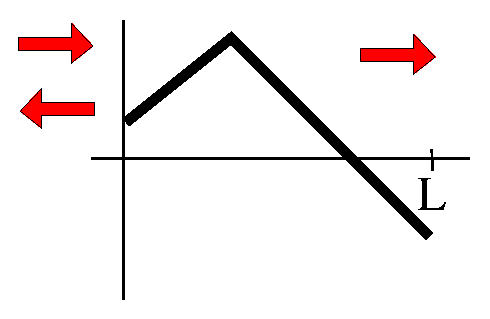
\includegraphics{pictures/transmission_derivation_14_LR}}
\scalebox{0.3}{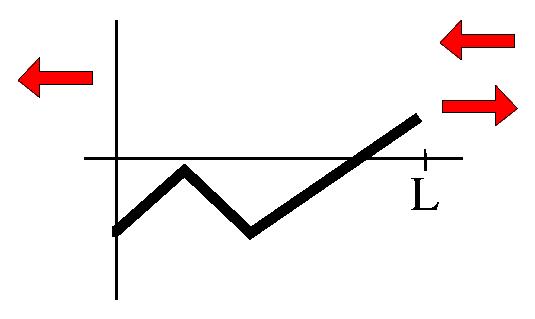
\includegraphics{pictures/transmission_derivation_34_RL}}}
\vskip -0.5cm
\caption{$\psi _1$ on the left and $\psi _2$ on the right for the passive models.}
\label{fig:alphabetacononicaldefectpositions}
\end{figure}

Similarily for $\tilde{ \psi} _1$ denoting the $\frac{1}{4}$L center of localization for left-to-right orientation and $\tilde{ \psi} _2$ being the $\frac{3}{4}$L center of localization for the right-to-left orientation.
%%20091214%%\section{single scatterer}

We derive the matrix for a single scatter in a quasi-1D channel of height w (where y goes from 0 to w) and the defect is at x = 0. The incident amplitude is A, reflection is B, and transmission is C.  These are later normalized to 1, r, and t, respectively.

For simplicity we assume there are two open channels (N=2) and two closed channels ($N_c$=2) and that the incident light is only in channel 2. The algorithm can be duplicated for any arbitrary open channel. It doesn't make sense to say the incident light is in the closed channel since those are not propagating modes. The algorithm show works for arbitrary number of open and closed channels. We show that closed channels can be ``folded'' into the open channels, which maintains conservation of information. The rank of the matrix is reduce from $N+N_c$ to N but the terms become messier.

Method for matrix setup: match boundary conditions for the amplitude and derivative at the scatterer.
% see Ben's notes, 20080617
The general equation describing the system is
\begin{equation}
A_2 \chi_2(y) \exp(i k_2 x) + \sum_{n=1}^4 B_n \chi_n(y) \exp(-i k_n x) = 
\sum_{n=1}^4 C_n \chi_n(y) \exp(i k_n x)
\label{singlescattererwave}
\end{equation}
where if $n>N$, then $k_n = i \kappa_n$.

Boundary condition: amplitudes match at x = 0. For each channel, multiply both sides by
\begin{equation}
\int dy \chi_m(y)
\end{equation}
which by orthogonality with $\chi_n(y)$ yields $\delta_{nm}$, so at x=0,
\begin{equation}
\begin{gathered}
B_1 = C_1 \\
A_2 + B_2 = C_2 \\
B_3 = C_3 \\
B_4 = C_4
\end{gathered}
\end{equation}

In order to have the derivatives match we detour to the Schr\"{o}dinger equation:

\begin{equation}
(-\frac{\hbar^2}{2 m}(\frac{d^2}{dx^2}+\frac{d^2}{dy^2})+\gamma \delta(x)\delta(y-y_o))\Psi = E \Psi
\end{equation}
(equation 1 in \cite{1990_Bagwell}).

separation of variables:
\begin{equation}
\Psi = \sum_n D_n(x) \chi_n(y)
\end{equation}

\begin{equation}
-\frac{\hbar^2}{2 m} \frac{d^2}{dy^2} \chi_n(y) = E_n \chi_n(y)
\end{equation}

boundary condition: $\chi_n(y)$ = 0 for y = 0 and y = w.

\begin{equation}
\begin{gathered}
\chi_n(y) = \sqrt{\frac{2}{w}sin(\frac{n \pi}{w}y} \\
E_n = \frac{\hbar^2}{2 m}(\frac{n \pi^2}{w})^2
\end{gathered}
\end{equation}

\begin{equation}
-\frac{\hbar^2}{2 m}\sum_m D_m^{''}(x) \chi_m(y) + 
\sum_m D_m(x) E_m \chi_m(y) + 
\gamma \delta(x) \sum_m D_m(x) \chi_m(y) \delta(y-y_o) = 
E_{total} \sum_m D_m(x) \chi_m(y)
\end{equation}
where $E_m \chi_m(y)$ = $\chi_m^{''}(y)$. Multiply both sides by 
$\int dy \chi_n(y)$ to get $\delta_{mn}$ which leads to 
\begin{equation}
-\frac{\hbar^2}{2 m} D_n^{''}(x) +D_n(x) E_n +
\delta(x) \sum_m D_m(x) \gamma \chi_n(y_o) \chi_m(y_o) = D_n(x) E
\end{equation}
re-arranging, we get Bagwell's equation 4,
\begin{equation}
\frac{d^2}{dx^2}D_n(x) + (\frac{E-E_n}{\hbar^2})D_n = 
\delta(x) \sum_m D_m(x) \Gamma_{nm}
\label{Bagwellsequ4}
\end{equation}
where
\begin{equation}
\begin{gathered}
k_n^2 = \frac{E-E_n}{\hbar^2}2 m \\
\Gamma_{nm} = \chi_n(y_o) \chi_m(y_o)
\end{gathered}
\end{equation}
Now we can match derivatives at x=0. Integrate over a small region, applying
\begin{equation}
\int_{0-\epsilon}^{0+\epsilon}dx
\end{equation}
to equation \ref{Bagwellsequ4}

\begin{equation}
\frac{dD_n}{dx}|^{+\epsilon}_{-\epsilon} + k_n^2 D_n 2 \epsilon = 
\sum_m D_m(0) \Gamma_{nm}
\end{equation}
which is Bagwell's equation 18. Now let $\epsilon \rightarrow$ 0
\begin{equation}
\frac{dD_n(+)}{dx} - \frac{dD_n(-)}{dx} = \sum_m^4 D_m(0) \Gamma_{nm}
\end{equation}
Where $D_{n}(+)$ is the derivative of the wave function x component on the left side of the scatterer, and similarly $D_{n}(+)$ is on the right side of the scatterer. Apply to equation \ref{singlescattererwave}
\begin{equation}
i k_n C_n - (i k_2 A_2 \delta_{2 n} - i k_n B_n) = 
\sum_{m=1}^4 C_m \Gamma_{nm}
\end{equation}
from the fist set of boundary conditions, $B_1=C_1$, $A_2+B_2=C_2$, $B_3=C_3$, $B_4=C_4$, thus $B_2=C_2-A_2$

For channels 1,3, and 4 =n
\begin{equation}
2 i k_n C_n = \sum_{m=1}^4 C_m \Gamma_{nm}
\end{equation}
and for channel 2,
\begin{equation}
\begin{gathered}
i k_2 (C_2 - A_2 +B_2) = i k_2 (C_2 -A_2 + (C_2 - A_2)) = 2 i k_2 (C_2 -A_2) = \sum C_m \Gamma_{2m} \\
-2 i k_2 A_2 = (\sum_m C_m \Gamma_{2m}) - 2 i k_2 C_2 \\
-2 i k_2 = (\sum_m (\frac{C_m}{A_2}) \Gamma_{2m}) - 2 i k_2 \frac{C_2}{A_2}
\end{gathered}
\end{equation}
Define $C_m/A_2$ as transmission $t_{2m}$ so that coefficients are normalized to incident unity. [Note: 1 with respect to each channel, so that if there are 2 input channels the incidence is actually 2 (?)]

The four sums can be written as a matrix
\begin{equation}
 \left( \begin{array}{c}
0 \\
-2 i k_2 \\
0 \\
0  \end{array} \right) =
 \left( \begin{array}{cccc}
\Gamma_{11}-2 i k_1 & \Gamma_{12}         & \Gamma_{13}              & \Gamma_{14} \\
\Gamma_{21}         & \Gamma_{22}-2 i k_2 & \Gamma_{23}              & \Gamma_{24} \\
\Gamma_{31}         & \Gamma_{32}         & \Gamma_{33}+2 i \kappa_3 & \Gamma_{34} \\
\Gamma_{41}         & \Gamma_{42}         & \Gamma_{43}              & \Gamma_{44}+2 i \kappa_4 \end{array} \right)
 \left( \begin{array}{c}
t_21 \\
t_22 \\
t_23 \\
t_24 \end{array} \right) 
\end{equation}

Where the left side vector is the input, and the right side matrix are the transmission coefficients. Note that there were two (open) input channels, which correspond to the upper 2 elements, and the lower elements correspond to the closed channels, which can not be inputs.
%%20091214%%\section{two scatterer folding}

Two scatterers: incident is A, reflected is B, and transmitted is G. Between are C (forward) and D (backward).

% see notes, 20080619
First, boundary conditions match for the amplitudes and the derivatives, where n is the single incident channel, which scatters into channels m. For the first scatterer,
\begin{equation}
\begin{gathered}
A_n \delta_{mn} + B_m = C_m+D_m \\
(i k_m C_m-i k_m D_m) - (i k_m \delta_{nm}^{(1)} A_m-i k_m B_m) = 
\sum_{m'} \Gamma_{mm'} (A_n \delta_{nm'}+B_{m'})
\end{gathered}
\end{equation}
and similarly for the second scatterer, which is at x=a instead of zero,
\begin{equation}
\begin{gathered}
C_m \exp(i k_m a) + D_m \exp(-i k_m a) = G \exp(i k_m a) \\
(i k G_m \exp(i k_m a)-(i k_m C_m \exp(i k_m a) - i k_m D_m \exp(-i k_m a)) = 
\sum_{m'} \Gamma_{mm'}^{(2)} G_{m'} \exp(i k_{m'} a)
\label{matchatxequalsa}
\end{gathered}
\end{equation}
the k variable is a matrix of diagonal elements indexed by channel number
\begin{equation}
\hat{k}_{nn} = \sqrt{(\frac{2 \pi}{\lambda})^2 -(\frac{\pi n}{w})^2}
\end{equation}
where n goes from 1 to $N+N_c$

\begin{equation}
\begin{gathered}
C_m +D_m = \delta_{mn} A_m+B_m \\
C_m -D_m = A_m \delta_{mn} - B_m +\frac{1}{i k_m} \sum_{m'} 
\Gamma_{mm'}^{(1)} (\delta_{nm'} A_{m'}+B_{m'})
\end{gathered}
\end{equation}
Solve for $C_m$ and $D_m$ at x = 0.
\begin{comment}
use
x+y=A
x-y=B
==>  2x = A+B
====> x = (A+B)/2
repeat for y
\end{comment}

\begin{equation}
\begin{gathered}
C_m = A_m \delta_{nm} + \frac{1}{2 i k_m}\sum_{m'}\Gamma_{mm'}^{(1)} 
(\delta_{nm'} A_{m'}+B_{m'}) \\
D_m = B_m - \frac{1}{2 i k_m}\sum_{m'}\Gamma_{mm'}^{(1)} 
(\delta_{nm'} A_{m'}+B_{m'})
\end{gathered}
\end{equation}
\begin{equation}
\begin{gathered}
A_m \delta_{nm} \exp(i k_m a)+B_m \exp(-i k_m a) + 
\frac{1}{k_m}(\sum_{m'}\Gamma_{mm'}^{(1)}(\delta_{nm'} A_{m'}+B_{m'})) sin(k_m a) = \\
G_m \exp(i k_m a) \\
G_m \exp(i k_m a) - (A_m \delta_{nm} \exp(i k_m a)-B_m \exp(-i k_m a) + 
\frac{1}{i k_m}(\sum_{m'}\Gamma_{mm'}^{(1)}(\delta_{nm'} A_{m'}+B_{m'})) cos(k_{m'} a) = \\
\frac{1}{i k_m}(\sum_{m'}\Gamma_{mm'}^{(2)} G_{m'} \exp(i k_{m'} a)) \\
\end{gathered}
\end{equation}
divide everything by $A_m$ to get normalized incident wave
\begin{equation}
\begin{gathered}
\delta_{nm} \exp(i k_m a)+r_{mn} \exp(-i k_m a) + 
\frac{1}{k_m}(\sum_{m'}\Gamma_{mm'}^{(1)}(\delta_{nm'}+r_{nm'})) sin(k_m a) = \\
t_{nm} \exp(i k_m a) \\
t_{nm} \exp(i k_m a) - (\delta_{nm} \exp(i k_m a)-r_{mn} \exp(-i k_m a) + 
\frac{1}{i k_m}(\sum_{m'}\Gamma_{mm'}^{(1)}(\delta_{nm'}+r_{nm'})) cos(k_{m'} a) = \\
\frac{1}{i k_m}(\sum_{m'}\Gamma_{mm'}^{(2)} t_{nm'} \exp(i k_{m'} a)) \\
\end{gathered}
\end{equation}
where 
\begin{equation}
\begin{gathered}
\frac{B}{A} \equiv r_{nm} \\
\frac{G}{A} \equiv t_{nm}
\end{gathered}
\end{equation}
Now we'll switch from indexed variable to matrix notation

\begin{equation}
\begin{gathered}
(\exp(-i \hat{k} a)+\hat{k}^{-1} sin(\hat{k} a) \hat{\Gamma}) \vec{r} + 
(-\exp(i \hat{k} a)) \vec{t} = \\
-(\exp(i \hat{k} a +\hat{k}^{-1} sin(\hat{k} a) \hat{\Gamma}) \vec{h}\\
(\exp(-i \hat{k} a)+i \hat{k}^{-1} cos(\hat{k} a) \hat{\Gamma}) \vec{r} + 
(\exp(i \hat{k} a)+i \hat{k}^{-1} \exp(i \hat{k} a) \hat{\Gamma}) \vec{t} = \\
(\exp(i \hat{k} a)-i \hat{k}^{-1} cos(\hat{k} a) \hat{\Gamma}) \vec{h}
\end{gathered}
\end{equation}
we clump the coefficients in that big mess to another indexed variable, ``F''.
\begin{equation}
\begin{gathered}
\hat{F_1} \vec{r}+\hat{F_2} \vec{t}=\hat{F_3} \vec{h} \\
\hat{F_4} \vec{r}+\hat{F_5} \vec{t}=\hat{F_6} \vec{h}
\end{gathered}
\end{equation}

solve for $\vec{r}$, set the two equal
\begin{equation}
\begin{gathered}
(\hat{F_1}^{-1} \hat{F_3}-\hat{F_4}^{-1} \hat{F_6}) \vec{h} = 
(\hat{F_1}^{-1} \hat{F_2}-\hat{F_4}^{-1} \hat{F_5}) \vec{t}
\end{gathered}
\end{equation}
then solve for $\vec{h}$ in terms of $\vec{t}$
\begin{equation}
\vec{h} = (\hat{F_1}^{-1} \hat{F_3} - \hat{F_4}^{-1} \hat{F_6})^{-1}
(\hat{F_1}^{-1} \hat{F_2} - \hat{F_4}^{-1} \hat{F_5}) \vec{t}
\end{equation}
and we'll call that big messy matrix, which has dimension $(N+N_c)x(N+N_c)$,
\begin{equation}
(\hat{F_1}^{-1} \hat{F_3} - \hat{F_4}^{-1} \hat{F_6})^{-1}
(\hat{F_1}^{-1} \hat{F_2} - \hat{F_4}^{-1} \hat{F_5}) \equiv
\hat{I}+\frac{i}{2}\hat{k}^{-1}\Gamma^{combined}
\end{equation}
Solving for $\Gamma^{combined}$, 
\begin{equation}
\Gamma^{combined} = -i 2\hat{k}(((\hat{F_1}^{-1} \hat{F_3} - \hat{F_4}^{-1} \hat{F_6})^{-1}
(\hat{F_1}^{-1} \hat{F_2} - \hat{F_4}^{-1} \hat{F_5})) - \hat{I})
\end{equation}

Now we have a general algorithm for combining any two $\Gamma$ matrices, either two reduced (open channels only, (NxN)) or two unreduced (open and closed channels, (($N+N_c$)x($N+N_c$))). 

Using this ``gamma combiner'' algorithm with the above ``gamma reducer'' algorithm we can numerically compute how the two are different, and how separation (density in many scatterers) is affected when N varies, when $N_c$ is include or not.
%\chapter{Characteristic Length Scales}
\label{sec:lengths}
%This table lists lengths used in the dissertation.

\captionsetup[table]{list=no}
%\begin{center}
\begin{table} % for label and caption purposes
%\begin{tabular}{|l|l|l|} % table runs off page
%\begin{tabular}{|l|l|p{7cm}|} % center column too large
\caption{Length scales used in this dissertation}
\begin{tabular}{|l|p{4cm}|p{8.5cm}|}
%\begin{tabular*}{0.75\textwidth}{|l|l|l|}{@{\extracolsep{\fill}} | c | c | c | }
\hline Symbol & Name & Description \\ \hline
$\lambda$ & wavelength & Wavelength of incident light \\ 
$L$ &  system length & Length of waveguide along direction of propagation ($z$-axis) \\ 
$W$ & system width & Dimension of waveguide perpendicular to direction of propagation ($y$-axis) \\
$L_{\phi}$ & phase coherence length & Length over which phase remains coherent. Equivalent to $L_{inelastic}$\cite{1988_Stone,1986_Imry}. Applicable only to electron transport. \\
$L_D$ & path length & How far a particle (i.e. ray optics) travels in the media in ballistic and diffusive regimes \\
$\ell_{scat}$ & scattering length & Average distance between scattering events. Often referred to as $\ell_{mfp}$ (mean free path) or the inelastic length\cite{1984_John_prl}, or extinction length\cite{1999_van_Tiggelen}. \\ 
$\ell_{tmfp}$ & transport mean free path & Average distance over which phase and direction are randomized.  $\ell_{tmfp} = \frac{\ell_{scat}}{1-\langle cos\ \theta \rangle}$. Sometimes referred to as elastic mfp\cite{1991_John}. % page 34, col 2
Measured with respect to $L$. \\ 
$\xi$ & localization length & Probability of diffusive path forming loop is 1. $\xi~=~N~\ell_{tmfp}$. Measured with respect to $L$. \\ 
$\ell_{a,g}$ & ballistic absorption/gain length & Average distance over which intensity decreases by two/increases by two. \\
$\xi_{a,g}$ & absorption/gain length & How far, on average, a particle travels in the diffusive regime before being absorbed (or doubled), measured with respect to path length $L_D$ in the diffusive regime \\ 
$z_p$ & penetration depth & Applies to diffusive regime only. $z_p \approx \ell_{tmfp}$ \\ 
\hline
\end{tabular}

\ \\ 

\label{tabl:lengths}
\end{table}
%\end{center}
All length scales (except $\lambda$) are normalized by wavelength. % lengths can be converted to equivalent times by $\ell = c t$
%\captionsetup[table]{list=yes}
%\chapter{Derivation of Transfer Matrices for Electric Field Propagation in Planar Quasi-1D Waveguide From Maxwell's Equations}
\chapter{Transfer Matrices for Electric Field Propagation}
\label{sec:appendix_derivation_transfer_matrices_quasi1d}

In the following derivation, the transfer matrix method\cite{1981_MacKinnon_scaling}\cite{1992_Pendry}\cite{2003_Kettemann} is developed from Maxwell's equations\cite{1999_Jackson} for metallic waveguides with scatterers. Before starting, assumptions necessary for the derivation are enumerated. 
\begin{itemize}
\item Metallic boundaries for the surfaces of the waveguide result in no leakage of electric field at the edges. These boundaries occur in the direction perpendicular to propagation $y$, which extends from $y=0$ to $y=W\lambda$. In the direction of propagation along $z$, the waveguide has open boundaries at $z=0$ and $z=L/\lambda$. The metallic boundaries are infinite along direction $x$.
\item Scattering potentials are initially assumed to be $\delta$-functions, and are later reduced to a finite sum of Fourier components. This scattering potential description gives rise to transport behavior similar to that in physical disordered media. 
%   \item non-physical
%   \item infinite number of closed channels
\item No inelastic scattering occurs; there is no energy loss due to scattering, and phase can remain coherent.% [scatterers only affect amplitude].
\item No noise (spontaneous emission) is included. The primary interest in the modeling the transition from phenomena described by diffusion to that of Anderson localization. %Also, experimentally noise can be suppressed. % CITE
%The transmission with gain will be slightly different compared to real output.
\item Only transverse-magnetic (TM) waves are assumed incident. The electric field oscillates perpendicular to the plane of the 2D waveguide~
%``For EM waves propagating in the $z,y$ plane, the $s$ ($E$ field parallel to the $x$ axis) and $p$ ($E$ field perpendicular to the $x$ axis) polarized waves can be described by two decoupled wave equations.'' 
\cite{1996_soukoulis_dis2d}.
\item The absorption and gain mechanism is purely mathematical: no atomic level modeling is included. This is the appeal of working in the mesoscopic regime, namely that atomic-based scattering descriptions are not necessary.
%\item %, other than the capability to be selectively incident on a specific channel.
%\item By choosing planar quasi-1D geometry (and thus scalar waves), we implicitly assume that polarization will not significantly alter transport phenomena. Although planar geometry may be experimentally realizable, it is not as popular as 3D quasi-1D
\end{itemize}
No input beam properties are initially assumed. The incident energy can be a plane wave, or any other distribution.

%\section{From Maxwell equations to wave equation}
%Starting with Maxwell's equations, the wave equation for electromagnetic waves is derived to demonstrate that only a single polarization is being studied. Ampere's Law (with current $\vec{J}=0$ and $D=\epsilon_0 E$)\cite{1999_Jackson}, %Eq. I.1b, page 2
%\begin{equation}
%\vec{\nabla} \times \vec{{\cal H}} = \epsilon_0 \frac{\partial\vec{E}}{\partial t}
%\label{eq:amperes_law}
%\end{equation}
%Faraday's Law \cite{1999_Jackson}, %Eq. I.1a, page 2]
%\begin{equation}
%\vec{\nabla} \times \vec{E} = -\mu_0 \frac{\partial\vec{{\cal H}}}{\partial t}
%\label{eq:faradays_law}
%\end{equation}
%Taking the temporal derivative of Eq.~\ref{eq:amperes_law}
%\begin{equation}
%\vec{\nabla} \times \frac{\partial\vec{{\cal H}}}{\partial t} = \epsilon_0 \frac{\partial^2\vec{E}}{\partial t^2}
%\label{eq:temporal_derivative_of_amperes_law}
%\end{equation}
%Taking the curl of Eq.~\ref{eq:faradays_law}
%\begin{equation}
% \vec{\nabla} \times \vec{\nabla} \times \vec{E} = -\mu_0 \left(\vec{\nabla} \times \frac{\partial\vec{{\cal H}}}{\partial t} \right)
%\label{eq:curl_of_faradays_law}
%\end{equation}
%Substitute Eq.~\ref{eq:temporal_derivative_of_amperes_law} into Eq.~\ref{eq:curl_of_faradays_law}
%\begin{equation}
%  \vec{\nabla} \times \vec{\nabla} \times \vec{E} = -\mu_0 \epsilon_0 \frac{\partial^2\vec{E}}{\partial t^2}
%\end{equation}
%Vector identity: $\vec{\nabla} \times \vec{\nabla} \times \vec{E} = \vec{\nabla} (\vec{\nabla}\cdot \vec{E})-\nabla^2 \vec{E}$. Since we assume no source, we have the wave equation

The wave equation can be derived from Maxwell's equations (not shown), yielding
\begin{equation}
\nabla^2 E = \frac{1}{c^2} \frac{\partial^2\vec{E}}{\partial t^2}
\label{eq:general_wave_equ}
\end{equation}
where $\mu_0 \epsilon_0 = \frac{1}{c^2}$. 
%[See 1996 Soukoulis et al PRB v53 n13 pg 8340, section II] 
% Eq.~\ref{eq:general_wave_equ} ``is identical with the scalar wave equation.'' The $p$-polarized wave equation involves ${\cal H}$.

\section{Time Independent Wave Equation}
Assuming electric field variables are separable,
\begin{equation}
E(\vec{r},t) = E(\vec{r}) e^{i\omega t}
\label{eq:separation_of_variables_E_field}
\end{equation}
the field is simplified by also assuming monochromatic and continuous wave (CW). Substituting  Eq.~\ref{eq:separation_of_variables_E_field} into the right side of Eq.~\ref{eq:general_wave_equ}, time dependence can be canceled. 
\begin{equation}
\nabla^2 E(\vec{r}) = - \frac{\omega^2}{c^2} E(\vec{r})
\label{eq:wave_equation_electric_field}
\end{equation}
where $\frac{\omega}{c}=k$. Although the following results will appear to be ``time independent,'' the time dependence can be reintroduced by multiplying both sides by $e^{i\omega t}$. Effectively the same as assuming $t=0$. 


\section{Separation of Variables}
Convert from general $\vec{r}$ to two-dimensional Cartesian coordinates (since the transfer matrices for a planar quasi-1D waveguide are desired): $\vec{r} = z \hat{i}+y\hat{j}$. Let $W\equiv$~width and $L\equiv$~length of waveguide.
%\begin{equation}
%\vec{r} = z \hat{i}+y\hat{j}
%\end{equation}
%and the Laplacian is
%\begin{equation}
%\nabla^2 = \frac{\partial^2}{\partial z^2} + \frac{\partial^2}{\partial y^2}
%\label{eq:laplacian_cartesian}
%\end{equation}

%unjustified claim
The $z$ and $y$ components of the field are independent, the separation of variables applies spatially.
\begin{equation}
E(\vec{r}) = E(z,y) = \sum^\infty_{n=1} E_n(z) \chi_n(y)
\label{eq:spacialseparation}
\end{equation}
where the sum is over all channels. For $\delta$-function scatterers, there can be an infinite number of closed channels.

Now the wave equation (Eq.~\ref{eq:wave_equation_electric_field}) is 
\begin{equation}
\nabla^2 E(z,y) = - \frac{\omega^2}{c^2} E(z,y)
\label{eq:wave_equation_electric_field_cartesian}
\end{equation}
Apply Laplacian %(Eq.~\ref{eq:laplacian_cartesian}) 
and separation (Eq.~\ref{eq:spacialseparation})
\begin{equation}
\sum^\infty_{n=1} \left[ \frac{\partial^2E_n(z)}{\partial z^2} \chi_n(y) + E_n(z) \frac{\partial^2 \chi_n(y)}{\partial y^2} \right] = \\
- \frac{\omega^2}{c^2} \sum^\infty_{n=1} E_n(z) \chi_n(y)
\label{eq:summation_variable_separation_cartesian}
\end{equation}

\section{Perpendicular Component Solution}
The solution to the differential equation perpendicular to the direction of propagation is found from the auxiliary equation for each channel
\begin{equation}
\left(\frac{\partial^2}{\partial y^2} + k_{\bot n}^2 \right) \chi_n(y) = 0
\end{equation}
Boundary conditions for metallic waveguide: Electric field $E$ is zero at the boundaries, $\chi_n(0) = \chi_n(W) = 0$.
%\begin{equation}
%\chi_n(0) = \chi_n(W) = 0
%\end{equation}
The normalized solution is the familiar
\begin{equation}
\chi_n(y) = \sqrt{\frac{2}{W}} \sin (k_{\bot n} y)
\end{equation}
where 
%\begin{equation}
$k_{\bot n} \equiv \frac{n \pi}{W}$. 
%\label{eq:k_perpendicular}
%\end{equation}
As a check of normalization, for $m=n$
\begin{equation}
\int^W_0 \chi_n^2(y) dy = \frac{2}{W} \int^W_0 \sin^2 (k_{\bot n} y) = \frac{2}{W} \frac{1}{2} W = 1
\end{equation}
and if $m \neq n$, solutions are orthogonal
\begin{equation}
\int^W_0 \chi_n(y)\chi_m(y) dy = 0
\end{equation}
Thus, for general $n$ and $m$,
\begin{equation}
\int^W_0 \chi_n(y)\chi_m(y) dy = \delta_{n,m}
\label{eq:convert_to_kronecker}
\end{equation}

\section{Parallel Component Solution}
For the solution parallel to the direction of propagation of Eq.~\ref{eq:wave_equation_electric_field_cartesian}, the $z$-component starts with
\begin{equation}
\frac{\partial^2 E_n(z)}{\partial z^2} - k_{\bot n}^2 E_n(z) = - \frac{\omega^2}{c^2} E_n(z)
\end{equation}
Re-arrange and introduce a new variable
\begin{equation}
\frac{\partial^2 E_n(z)}{\partial z^2} + k_{\parallel n}^2 E_n(z) = 0
\label{eq:zcomponentdiffequ}
\end{equation}
where
\begin{equation}
k_{\parallel n}^2 \equiv \frac{\omega^2}{c^2} - k_{\bot n}^2
\label{eq:k_parallel}
\end{equation}
Note: $k_{\parallel n}^2$ can be positive (corresponding to open channels) or negative (closed channels). If negative, then $k_{\parallel n}$ is imaginary, denoted $k_{\parallel n} = i \kappa_{\parallel n}$ for $n > N_{open}$. Open channels propagate forward, with velocity decreasing as channel index increases. Closed channels decrease in amplitude exponentially.

%The summation in Eq.~\ref{eq:summation_variable_separation_cartesian} can be split into open and closed channels
%\begin{equation}
%\sum_{n=1}^\infty = \sum_{n=1}^{N_o} + \sum_{n=N_{o}+1}^\infty	
%\end{equation}

%\begin{tabular}{cc}
%$ n \leq N_o $ \quad \quad \quad & $ k_{\parallel n}^2 = \frac{\omega^2}{c^2} - \left(\frac{n \pi}{W}\right)^2 > 0 $ \\
%$ n > N_o $ \quad \quad \quad & $ k_{\parallel n}^2 < 0 $ \\
%\end{tabular}

Separate electric field components into left(-) and right (+) traveling plane waves (two solutions to the second order differential equation)
\begin{equation}
\begin{gathered}
\text{Open: \ }  E_n(z) = E_n^+ \exp(i k_{\parallel n} z) + E_n^- \exp(-i k_{\parallel n} z) \\
\text{Closed: \ }   E_n(z) = E_n^+ \exp(-\kappa_{\parallel n} z) + E_n^- \exp(\kappa_{\parallel n} z) 
\end{gathered}
\label{eq:Eleftandrightpropagating}
\end{equation}
where $i \kappa \equiv k$

\section{Waveguide With Scatterers}
Up to this point, an empty waveguide has been considered. For scattering, replace $\frac{\omega^2}{c^2}$ of the wave equation \ref{eq:wave_equation_electric_field_cartesian} with a spacial Sellmeier equation
\begin{equation}
\frac{\omega^2}{c^2} (1 + \alpha \delta(z-z_0,y-y_0))
\label{eq:scatterer}
\end{equation}
where $\delta(z-z_0,y-y_0) \equiv \delta(z-z_0) \delta(y-y_0)$ is the scattering potential and $\alpha$ is the scattering strength. $\alpha$ can be complex; then the real part is the strength and the imaginary component is gain or absorption.

%Note: this new term changes Eqs.~\ref{eq:amperes_law},\ref{eq:general_wave_equ}, and \ref{eq:wave_equation_electric_field} by introducing a non-unity refractive index.

To determine transport of light past a scattering potential, apply continuity of electric field $E$ and its derivative. The following carries out matching component-wise derivative.

Assuming the scattering potential is located at cross-section $z$ (inside the waveguide $0<z<L$), and the electric field just before or after the scatterer (at $z \pm \Delta$) is a sum of independent channel components.
\begin{equation}
E(z \pm \Delta, y) = \sum_{n=1}^\infty E_n(z \pm \Delta) \chi_n(y)
\end{equation}
Applying Eq.~\ref{eq:scatterer} to Eq.~\ref{eq:zcomponentdiffequ}, the wave equation becomes
\begin{equation}
\sum_{n=1}^\infty \left( E_n^{\prime\prime} \chi_n + k_{\parallel n}^2 E_n \chi_n + \alpha \frac{\omega^2}{c^2} \delta(z-z_0,y-y_0) E_n \chi_n \right) = 0
\label{eq:doubleprimeEz}
\end{equation}

Multiply Eq.~\ref{eq:doubleprimeEz} by $ \chi_m $ and $ \int_0^W dy $. By applying Eq.~\ref{eq:convert_to_kronecker} and letting $A_{m,n}(y_0)=\chi_m(y_0) \chi_n(y_0)$, 
\begin{equation}
\sum_{n=1}^\infty \left( E_n^{\prime\prime} \delta_{nm} + k_{\parallel n}^2 E_n \delta_{nm} + \alpha \frac{\omega^2}{c^2} E_n \delta(z_0) A_{nm}(y_0)  \right) = 0 
\end{equation}
Apply the summation over $n$, which eliminates the Kronecker deltas.
\begin{equation}
 E_m^{\prime\prime} + k_{\parallel m}^2 E_m + \alpha \frac{\omega^2}{c^2} E_n \delta(z-z_0) \sum_{n=1}^\infty A_{nm}(y_0) = 0
\end{equation}
Integrate over $z$ from $(z-\Delta)$ to $(z+\Delta)$ and let $\Delta\rightarrow0$.
\begin{equation}
\begin{gathered}
\int_{z_0-\Delta}^{z_0+\Delta} E_m^{\prime\prime}(z) dz + k_{\parallel m} ^2 \int_{z_0-\Delta}^{z_0+\Delta} 
E_m(z) dz +\\ \alpha \frac{\omega^2}{c^2} \sum_{n=1}^\infty A_{n,m}(y_0) \int_{z_0-\Delta}^{z_0+\Delta} \delta(z_0) E_n dz = 0
\end{gathered}
\end{equation}

To do the second term integration, assume that for small $\Delta$, $E(z) \approx E(z_0)$.  
\begin{equation}
E_m^{\prime}(z_0 + \Delta) - E_m^{\prime}(z_0 - \Delta) + k_{\parallel m}^2 E_m(z_0) 2 \Delta + \alpha \frac{\omega^2}{c^2} \sum_{n=1}^\infty A_{n,m}(y_0) E_n(z_0) = 0
\end{equation}

Since $\Delta \rightarrow 0$, then $2 \Delta$ is really small, so that term is dropped.

To conclude, for a given channel $m$, electric field and the field derivative on both sides of the scatterer must match
\begin{equation}
\begin{gathered}
%\boxed{
E_m(z_0+\Delta) = E_m(z_0-\Delta) \\
%}
%\\
%\boxed{
E_m^{\prime}(z_0+\Delta) = E_m^{\prime}(z_0-\Delta) - \alpha \frac{\omega^2}{c^2} \sum_{n=1}^\infty A_{n,m}(y_0) E_n(z_0)
%}
\end{gathered}
\end{equation}

Note that the $\delta$ function scatterer has been eliminated, and $A_{n,m}$ can form an array (the ``scattering matrix'').

\begin{equation}
\begin{gathered}
\left( \begin{array}{cc}
\hat{I} & 0 \\
-\alpha \frac{\omega^2}{c^2}A_{mn}(y_0) & \hat{I} \\
\end{array} \right)
\left( \begin{array}{c}
E_{1..N_{max}}(z_0-\Delta) \\
\frac{1}{\kappa_{\parallel 1..N_{max}}} E_{1..N_{max}}^{\prime}(z_0-\Delta) 
\end{array} \right)
=\\
\left( \begin{array}{c}
E_{1..N_{max}}(z_0+\Delta) \\
\frac{1}{\kappa_{\parallel 1..N_{max}}} E_{1..N_{max}}^{\prime}(z_0+\Delta) 
\end{array} \right)
\end{gathered}
\end{equation}
Due to the form of the matrix, the determinant is always unity (only the diagonal contributes non-zero terms) regardless of the elements in the lower left quadrant. Elements of the lower left quadrant are
\begin{equation}
 -\alpha \frac{\omega^2}{c^2} \frac{2}{W} \sin(k_{\perp m} y_0) \sin(k_{\perp n} y_0)
\end{equation}
Note that the scattering matrix is real unless $\alpha$ or $\omega$ are complex.

\section{Free Space Propagation of Open Channels}
For open channels ($n \leq N_o$), field $E_n$ and derivative of field $ \frac{1}{k_{\parallel n}}E_n^{\prime}$ are more convenient basis than ``left traveling'' $E_n^-(z)$ and ``right traveling'' $E_n^+(z)$. First, the connection between the two basis is found. Starting from Eq.~\ref{eq:Eleftandrightpropagating}, electric field $E(z)$ is the solution to a second order differential equation, so it has two solutions.
\begin{equation}
\begin{gathered}
E_n(z) = E_n^+ \exp(i k_{\parallel n} z) + E_n^- \exp(-i k_{\parallel n} z) \\
E_n^{\prime}(z) = i k_{\parallel n} E_n^+ \exp(i k_{\parallel n} z) - i k_{\parallel n}E_n^- \exp(-i k_{\parallel n} z)
\label{eq:Eleftandrightpropagating_again}
\end{gathered}
\end{equation}
Solving for left- and right-traveling wave components,
\begin{equation}
\begin{gathered}
E_n^+(z) = \frac{1}{2} \left( E_n(z)+\frac{1}{i} \frac{1}{k_{\parallel n}} E_n^{\prime}(z) \right) \exp(-i k_{\parallel n} z) \\ 
E_n^-(z) = \frac{1}{2} \left( E_n(z)-\frac{1}{i} \frac{1}{k_{\parallel n}} E_n^{\prime}(z) \right) \exp(i k_{\parallel n} z) 
\label{eq:Eleftright}
\end{gathered}
\end{equation}

To preemptively clear up notation confusion, in previous steps $\Delta$ was used to denote a small ($\Delta \rightarrow 0$) distance from the scatterer. Here $\Delta z$ will be used to signify a finite displacement in position along the $z$ axis. 

The field and derivative of field is translated over distance $\Delta z$ from the original position $z$. First, substitute the shift into Eq.~\ref{eq:Eleftandrightpropagating_again}
\begin{equation}
E_n(z+\Delta z) = E_n^+ \exp(i k_{\parallel n} (z+\Delta z)) + E_n^- \exp(-i k_{\parallel n} (z+\Delta z)) 
\end{equation}
Then substitute Eq.~\ref{eq:Eleftright}
\begin{equation}
\begin{gathered}
E_n(z+\Delta z) = \frac{1}{2} \left( E_n(z) + \frac{1}{i} \frac{1}{k_{\parallel n}} E_n^{\prime}(z) \right) \exp(i k_{\parallel n} z) + \\
\frac{1}{2} \left( E_n(z) - \frac{1}{i} \frac{1}{k_{\parallel n}} E_n^{\prime}(z) \right) \exp(-i k_{\parallel n} z) 
\end{gathered}
\end{equation}
Reducing leaves how to shift an electric field over distance $\Delta z$.
\begin{equation}
%\boxed{
E_n(z+\Delta z) =E_n(z) \cos(k_{\parallel n} \Delta z) + \frac{1}{k_{\parallel n}} E_n^{\prime} \sin(k_{\parallel n} \Delta z) 
%}
\label{eq:open_channel_field_transfer}
\end{equation}
Similarly,
\begin{equation}
\frac{1}{k_{\parallel n}} E_n^{\prime}(z+\Delta z) = i E_n^+ \exp(i k_{\parallel n} (z+\Delta z)) -i E_n^- \exp(-i k_{\parallel n} (z+\Delta z))
\end{equation}
Then substitute Eq.~\ref{eq:Eleftright}
\begin{equation}
\begin{gathered}
\frac{1}{k_{\parallel n}} E_n^{\prime}(z+\Delta z) =
\frac{i}{2} \left( E_n(z) + \frac{1}{i} \frac{1}{k_{\parallel n}} E_n^{\prime}(z) \right) \exp(i k_{\parallel n} z) -\\
\frac{i}{2} \left( E_n(z) - \frac{1}{i} \frac{1}{k_{\parallel n}} E_n^{\prime}(z) \right) \exp(-i k_{\parallel n} z) 
\end{gathered}
\end{equation}

\begin{equation}
%\boxed{
\frac{1}{k_{\parallel n}} E^{\prime}(z+\Delta z)=- E_n(z) \sin(k_{\parallel n} \Delta z) + \frac{1}{k_{\parallel n}} E_n^{\prime} \cos(k_{\parallel n} \Delta z) 
%}
\label{eq:open_channel_deriv_transfer}
\end{equation}

\section{Free-space Propagation of Closed Channels}
For closed channels ($n > N_o$), change of $i$ results in hyperbolic trig functions.
\begin{equation}
\begin{gathered}
E_n(z) = E_n^+ \exp(-\kappa_{\parallel n} z) + E_n^- \exp(\kappa_{\parallel n} z) \\
E_n^{\prime}(z) = -\kappa_{\parallel n} E_n^+ \exp(-\kappa_{\parallel n} z) + \kappa_{\parallel n}E_n^- \exp(\kappa_{\parallel n} z)
\end{gathered}
\end{equation}
Recalling that $k_{\parallel n} = i \kappa_{\parallel n}$, then
\begin{equation}
\begin{gathered}
E_n^+(z) = \frac{1}{2} \left( E_n(z)- \frac{1}{\kappa_{\parallel n}} E_n^{\prime}(z) \right) \exp(\kappa_{\parallel n} z) \\ 
E_n^-(z) = \frac{1}{2} \left( E_n(z)+ \frac{1}{\kappa_{\parallel n}} E_n^{\prime}(z) \right) \exp(-\kappa_{\parallel n} z) 
\end{gathered}
\end{equation}

Shifting the field by $\Delta z$
%\begin{equation}
%E_n(z+\Delta z) = E_n^+ \exp(-\kappa_{\parallel n}(z+\Delta z)) + E_n^- \exp(\kappa_{\parallel n}(z+\Delta z))
%\end{equation}
%\begin{equation}
%E_n(z+\Delta z) = \frac{1}{2} \left( E_n(z)- \frac{1}{\kappa_{\parallel n}} E_n^{\prime}(z) \right) \exp(-\kappa_{\parallel n} z) +  
%\frac{1}{2} \left( E_n(z)+ \frac{1}{\kappa_{\parallel n}} E_n^{\prime}(z) \right) \exp(\kappa_{\parallel n} z) 
%\end{equation}
\begin{equation}
%\boxed{
E_n(z+\Delta z) = E_n(z) \cosh(\kappa_{\parallel n}\Delta z) + \frac{1}{\kappa_{\parallel n}} E_n^{\prime}(z) \sinh(\kappa_{\parallel n}\Delta z)
%}
\end{equation}
and
%\begin{equation}
%\frac{1}{\kappa_{\parallel n}}E_n^{\prime}(z+\Delta z) = -E_n^+ \exp(-\kappa_{\parallel n}(z+\Delta z)) + E_n^- \exp(\kappa_{\parallel n}(z+\Delta z)) 
%\end{equation}
%\begin{equation}
%\begin{gathered}
%\frac{1}{\kappa_{\parallel n}}E_n^{\prime}(z+\Delta z) =-\frac{1}{2} \left( E_n(z)- \frac{1}{\kappa_{\parallel n}} E_n^{\prime}(z) \right) \exp(-\kappa_{\parallel n} z) + \\
%\frac{1}{2} \left( E_n(z)+ \frac{1}{\kappa_{\parallel n}} E_n^{\prime}(z) \right) \exp(\kappa_{\parallel n} z) 
%\end{gathered}
%\end{equation}
\begin{equation}
%\boxed{
\frac{1}{\kappa_{\parallel n}}E_n^{\prime}(z+\Delta z) =E_n(z) \sinh(\kappa_{\parallel n}\Delta z) + \frac{1}{\kappa_{\parallel n}} E_n^{\prime}(z) \cosh(\kappa_{\parallel n}\Delta z)
%}
\end{equation}

To summarize,
\begin{equation}
\begin{gathered}
E_n(z+\Delta z) = E_n(z) \cosh(\kappa_{\parallel n}\Delta z) + \frac{1}{\kappa_{\parallel n}} E_n^{\prime}(z) \sinh(\kappa_{\parallel n}\Delta z) \\
\frac{1}{\kappa_{\parallel n}}E_n^{\prime}(z+\Delta z) =E_n(z) \sinh(\kappa_{\parallel n}\Delta z) + \frac{1}{\kappa_{\parallel n}} E_n^{\prime}(z) \cosh(\kappa_{\parallel n}\Delta z)
\label{eq:closed_channel_transfer}
\end{gathered}
\end{equation}

From Eq.~\ref{eq:open_channel_field_transfer}, \ref{eq:open_channel_deriv_transfer}, and \ref{eq:closed_channel_transfer} the ``free space propagation matrix'' can be constructed. The array would be of rank $2 n_{max}$ ($n_{max}=N_o+N_c$). The determinant of this matrix is alway unity (regardless of argument) because terms can be factored into $\sin^2x +\cos^2=1$ for each channel. Thus, for both free and scattering matrices, the determinant is unity regardless of free space separation $\Delta z$ or real (passive) and complex (active media) dielectric values.

With this description of matrices for scattering planes and for free space propagation, the transmission of electric field and its derivative can be computed for a metallic waveguide containing arbitrarily placed scatterers. The set of matrices is multiplied together to form a matrix $\hat{S}$ of size $2n_{max}$. Then the vector describing the initial incident field and derivative of field for each channel $n$ is multiplied by $\hat{S}$ to give the transmission and reflection matrices (one vector for each channel $n$).

This approach of multiply matrices together inherently results in numerical instability~\cite{1968_Osedelec} due to the limited precision of computational devices. Therefore, the self-embedding technique~\cite{1999_yamilov_selfembed,1976_Bellman_Wing_embedding} is used to periodically renormalize the product.

\begin{comment}
\begin{equation}
\left( \begin{array}{cccccccc}
\cos(k_{\parallel 1}\Delta z)   & 0 & 0 & 0 & \sin(k_{\parallel 1}\Delta z)   & 0 & 0 & 0 \\
0 & \cos(k_{\parallel N_0}\Delta z) & 0 & 0 & 0 & \sin(k_{\parallel N_0}\Delta z) & 0 & 0 \\

0 & 0 & \cosh(k_{\parallel N_0+1}\Delta z)   & 0 & 0 & 0 & \sinh(k_{\parallel n}\Delta z) & 0  \\
0 & 0 & 0 & \cosh(k_{\parallel n_{max}}\Delta z) & 0 & 0 & 0 & \sinh(k_{\parallel n}\Delta z) \\

-\sin(k_{\parallel n}\Delta z) & 0 & \cos(k_{\parallel n}\Delta z) & 0 \\
-\sin(k_{\parallel n}\Delta z) & 0 & \cos(k_{\parallel n}\Delta z) & 0 \\

0 & \sinh(k_{\parallel n}\Delta z) & 0 & \cosh(k_{\parallel n}\Delta z) \\
0 & \sinh(k_{\parallel n}\Delta z) & 0 & \cosh(k_{\parallel n}\Delta z) \\
\end{array} \right)
\end{equation}

\begin{equation}
\left( \begin{array}{cccc}
\cos(k_{\parallel 1..N_0}\Delta z)  & 0 & \sin(k_{\parallel 1}\Delta z) & 0 \\
0 & \cosh(k_{\parallel N_0+1..n_{max}}\Delta z) & 0 & \sinh(k_{\parallel N_0+1..n_{max}}\Delta z)  \\
-\sin(k_{\parallel 1..N_0}\Delta z) & 0 & \cos(k_{\parallel 1..N_0}\Delta z) & 0 \\
0 & \sinh(k_{\parallel N_0+1..n_{max}}\Delta z) & 0 & \cosh(k_{\parallel N_0+1..n_{max}}\Delta z) \\
\end{array} \right)
\left( \begin{array}{c}
E_1 \\
\vdots \\
E_N \\	
E_{N+1} \\
\vdots \\
E_{N_{max}} \\
\frac{1}{k_{\parallel 1}} E_1^{\prime} \\
\vdots \\
\frac{1}{k_{\parallel N}} E_N^{\prime} \\
\frac{1}{\kappa_{\parallel N+1}} E_{N+1}^{\prime} \\
\vdots \\
\frac{1}{\kappa_{\parallel N_{max}}} E_{N_{max}}^{\prime} 
\end{array} \right)
\end{equation}
Note that the derivative portion of the free space propagation is where ``energy loss'' occurs (in passive $N_{open}$ systems). 


\section{Boundary Condition}

\begin{equation}
v(z) = 
\left( \begin{array}{c}
E_1 \\
\vdots \\
E_N \\	
E_{N+1} \\
\vdots \\
E_{N_{max}} \\
\frac{1}{k_{\parallel 1}} E_1^{\prime} \\
\vdots \\
\frac{1}{k_{\parallel N}} E_N^{\prime} \\
\frac{1}{\kappa_{\parallel N+1}} E_{N+1}^{\prime} \\
\vdots \\
\frac{1}{\kappa_{\parallel N_{max}}} E_{N_{max}}^{\prime} 
\end{array} \right)
= \left( \begin{array}{c}
\vec{E}_{open}(z) \\
\vec{E}_{closed}(z) \\
\vec{D}_{open}(z) \\
\vec{D}_{open}(z) \\
\end{array} \right)
\end{equation}

\begin{equation}
\hat{M}(0,L) \vec{v}(0) = \vec{v}(L)
\end{equation}

\begin{equation}
 E(y,z,t) = \left\{
\begin{array}{l l}
E_{in} e^{i(\vec{r}\cdot \vec{k} - \omega t)} + E_{r} e^{-i(\vec{r}\cdot \vec{k} + \omega t)} & \quad \mbox{ if $x<0$} \\
E_t e^{i(\vec{r}\cdot \vec{k} - \omega t)}  & \quad \mbox{ if $x>L$} \\ \end{array} \right.
\end{equation}

The transmission coefficient is $T=\frac{|E_t|^2}{|E_{in}|^2}$.
\end{comment}


\chapter{\texorpdfstring{Relation of $T/{\cal E}$}{T/E} to \texorpdfstring{$D(z)$}{D(z)}} %  From Self-consistent Theory of Anderson Localization
\label{sec:appendix_TE_Dz_relation}

% see also lab notebook SVN 20091230_ben_transmission_energy_derivations
% Note: a significant amount of content was barrowed from /svn/research/oned/TE\_paper

This is an expansion of Appendix section~\ref{app:Dz_derivation}. As in that section we assume a slab geometry. The $z$ coordinate normal to the slab is separated from the perpendicular component ${\bf \rho}$ as ${\bf r}=({\bf \rho},z)$. Again assuming no dependence on ${\bf \rho}$ allows us to give the ensemble-averaged diffusive flux $\langle\vec{J}(\vec{r},t)\rangle$ and the energy density $\langle {\cal W}(\vec{r},t)\rangle$ are related via \cite{1953_Morse}
\begin{equation}
\langle\vec{J}(\vec{r},t)\rangle=-D(\vec{r})\vec{\nabla}\langle {\cal W}(\vec{r},t)\rangle
\label{eq:Jflux_relation}
\end{equation}
The diffusion approximation amounts to $D(\vec{r})\equiv D_0=c\ell_{tmfp}/3$, where $c$ is the speed of light and $\ell_{tmfp}$ is the transport mean free path.

We consider a 3D random medium in a shape of a slab of thickness $L$, where we explicitly  separate the coordinate $z$ normal to the slab from the perpendicular component ${\bf \rho}$ as ${\bf r}=({\bf \rho},z)$. Under a CW plane-wave illumination at normal incidence, the dependence on ${\bf \rho}$ and $t$ can be neglected. 
\begin{equation}
\langle\vec{J}_z(z)\rangle=-D(z)\frac{d}{dz}\langle {\cal W}(z)\rangle
\end{equation}

Integration over $z$ gives
\begin{equation}
\int_z^L\frac{\langle J_z(z^\prime)\rangle dz^\prime}{D(z^\prime)}=-\langle {\cal W}(L)\rangle + \langle {\cal W}(z)\rangle
\label{eq:E1_relation}
\end{equation}
where the energy stored inside the random medium ${\cal E}$ is formally defined as
\begin{equation}
\langle {\cal E} \rangle =\int_0^L\langle {\cal W}(z)\rangle dz.
\label{eq:Energy_definition_relation}
\end{equation}
thus
\begin{equation}
\langle {\cal E} \rangle = \int_0^L \left( \langle {\cal W}(L)\rangle + \int_z^L\frac{\langle J_z(z^\prime)\rangle }{D(z^\prime)}dz^\prime\right) dz
\end{equation}
The remaining work is to factor out transmission $T$ in order to find the relation between $T/{\cal E}$ and $D(z)$. The energy density $\langle {\cal W}(L)\rangle$ at the right boundary can be expressed in terms of right- and left-propagating fluxes. From the definition of diffusive flux \cite{1953_Morse}
\begin{equation}
\langle J_{\pm}(z)\rangle = \frac{c}{4} \langle {\cal W}(z)\rangle \mp \frac{D_0}{2} \frac{d\langle {\cal W}(z)\rangle }{dz}
\label{eq:diffusive_flux_relation}
\end{equation}
where $ \langle J_{-}\rangle$ and $ \langle J_{+}\rangle $ are the fluxes propagating along negative and positive $z$-directions respectively. Since $\langle J_+(L)\rangle=J_0T$ and $\langle J_-(L)\rangle=0$, using Eqs.~\ref{eq:diffusive_flux_relation} to eliminate $D_0$ yields
\begin{equation}
\langle J_+(L)\rangle + \langle J_-(L)\rangle = 2 \frac{c}{4}\langle {\cal W}(L)\rangle
\end{equation}
Therefore $\langle {\cal W}(L)\rangle=2J_0T/c$ and the energy can be re-written as
\begin{equation}
\langle {\cal E} \rangle = \int_0^L \left( 2J_0T/c + \int_z^L\frac{\langle J_z(z^\prime)\rangle}{D(z^\prime)}dz^\prime\right) dz
\end{equation}
Next, we reduce $\langle J_z(z^\prime)\rangle$ to find an approximately equivalent transmission.

%the boundary conditions are from Eq.~\ref{eq:Jflux_conserv}
%\begin{equation}
%J_z(z=0)=-J_0R,\ \, J_z(z=L)=J_0T
%\label{eq:Jflux_bc}
%\end{equation}

In the CW regime when the energy density ${\cal W}(z)$ is stationary, $\partial \langle {\cal W}(z)\rangle/\partial t=0$, it follows from energy conservation condition for flux $\vec{J}$ and energy ${\cal W}$
\begin{equation}
\frac{\partial \langle {\cal W}(\vec{r},t)\rangle }{\partial t}+\vec{\nabla} \cdot \langle\vec{J}(\vec{r},t)\rangle=
\frac{c}{\ell_g}\langle {\cal W}(\vec{r},t)\rangle+J_0 \delta(z-z_p)
\label{eq:Jflux_conserv_relation}
\end{equation}
 that the $z$ component of flux is constant for $z>z_p\sim\ell$. The value of the constant can be obtained from the boundary condition at $z=L$ as
\begin{equation}
\langle J_z(z)\rangle=\left\{
\begin{array}{l l}
\langle J_z(L)\rangle\equiv J_0 \langle T \rangle ,&\quad z_p<z<L\\
\langle J_z(0)\rangle\equiv -J_0 \langle R \rangle,&\quad 0<z<z_p\\
\end{array} \right.
\label{eq:Jfluxz_const_relation}
\end{equation}
where $T$ ($R$) is the transmission (reflection) coefficient. As a check, by integrating Eq.~(\ref{eq:Jflux_conserv_relation}) over the entire system we obtain the standard (passive) flux conservation $\langle J_z(L)\rangle -\langle J_z(0)\rangle =J_0 \langle T \rangle-(-J_0 \langle R \rangle)=J_0(\langle T \rangle+\langle R \rangle)=J_0$. To take advantage of the fact that $\langle J_z(z)\rangle$ is piecewise constant, c.f. Eq.~(\ref{eq:Jfluxz_const_relation}), we have to neglect by $0<z<z_p$ contribution. Then a constant can be substituted for $J_z(z')$,
\begin{equation}
\langle {\cal E} \rangle = \int_0^L \left( 2J_0\langle T \rangle/c + \int_z^L\frac{J_0 \langle T \rangle }{D(z^\prime)}dz^\prime\right) dz
\end{equation}
This introduces an error $\propto z_p/L\sim\ell/L\ll 1$. Factoring $T$ from the integrands,
\begin{equation}
\langle {\cal E} \rangle =J_0\langle T \rangle\int_0^L \left( \int_z^L\frac{dz^\prime}{D(z^\prime)}+2/c\right) dz
\label{eq:E1a_relation}
\end{equation}
Note that the second term is of the same order $\sim \ell/L$ as the term omitted in arriving to the above expression. Hence, $2/c$ contribution has to be dropped as well.
\begin{equation}
\langle {\cal E} \rangle =J_0T\int_0^L \int_z^L \frac{1}{D(z^\prime)}dz^\prime dz
\end{equation}

Taking advantage of the system symmetry, $D(z)=D(L-z)$, the double integration can be further simplified as
\begin{eqnarray}
\displaystyle\int_{0}^{L}\int_{z}^{L}\displaystyle\frac{1}{D(z^\prime)}dz^\prime dz &=&\frac{1}{2}\displaystyle\int_{0}^{L}\int_{0}^{L}\displaystyle\frac{1}{D(z^\prime)}dz^\prime dz \nonumber\\
&=&\frac{L}{2}\int_{0}^{L}\displaystyle\frac{1}{D(z)}dz.
\label{eq:E3_relation}
\end{eqnarray}
After normalizing the integral so that it yields unity in the case when the wave interference effects are neglected, $D(z)=D_0\equiv c\ell/3$, for passive media
\begin{equation}
\frac{\langle T \rangle}{\langle {\cal E} \rangle}\simeq
\frac{1}{J_0}
\frac{2D_0}{L^2}
\left(
\displaystyle\frac{1}{L}\displaystyle\int_{0}^{L}\displaystyle\frac{D_0}{D(z)}dz
\right)^{-1},
\label{eq:TE_vs_D_relation}
\end{equation}
We note that in process of deriving Eq.~(\ref{eq:TE_vs_D_relation}), we dropped the terms on the order of $\sim\ell/L\ll 1$.


Dropping the localization corrections leaves
\begin{equation}
\frac{\langle T \rangle}{\langle {\cal E} \rangle}\simeq \frac{1}{J_0} \frac{2D_0}{L^2}
\label{eq:diffusion_te_only}
\end{equation}
Any deviation from Eq.~\ref{eq:diffusion_te_only} in passive diffusive media can be attributed to localization corrections.

%%20091214%%\section{closed channel transfer matrix folding}

Now that we have a matrix of size $(N+N_c)x(N+N_c)$ it would be convenient to be able to represent it as a matrix of size $NxN$.  We will call this reduction "folding" as we are folding the closed channels into a smaller matrix. There is conservation of information in this matrix of reduced rank as the elements are messier.  The folding operation occurs one closed channel at a time, but it is shown by a recursion relation that the operation can be done by induction for an infinite number of closed channels.

Bagwell does the operation but gives an incorrect recursion relation. See~\cite{1990_Bagwell} page 358, equation 25.

dealing with a 4x4 matrix (2 open and 2 closed channels), solve for $t_{24}$ in the fourth equation:
\begin{equation}
t_{24} = -\frac{\Gamma_{41}}{\Gamma_{44}+2\kappa_4} t_{21} + 
         -\frac{\Gamma_{42}}{\Gamma_{44}+2\kappa_4} t_{22} +
         -\frac{\Gamma_{43}}{\Gamma_{44}+2\kappa_4} t_{23}
\end{equation}
then plug that into the three remaining equations. Group like terms
\begin{equation}
0 = ((\Gamma_{11}-\frac{\Gamma_{14}\Gamma_{41}}{\Gamma_{44}+2 \kappa_4}) - 2 i k_1)t_{21} + 
     (\Gamma_{12}-\frac{\Gamma_{14}\Gamma_{42}}{\Gamma_{44}+2 \kappa_4})t_{22} + 
     (\Gamma_{13}-\frac{\Gamma_{14}\Gamma_{43}}{\Gamma_{44}+2 \kappa_4})t_{23}  
\end{equation}
Now we can write a 3x3 matrix
\begin{equation}
 \left( \begin{array}{c}
0 \\
-2 i k_2 \\
0 \end{array} \right) =
 \left( \begin{array}{cccc}
(\Gamma_{11}-\frac{\Gamma_{14}\Gamma_{41}}{\Gamma_{44}+2 \kappa_4})-2 i k_1 &
(\Gamma_{12}-\frac{\Gamma_{14}\Gamma_{42}}{\Gamma_{44}+2 \kappa_4})           & 
(\Gamma_{13}-\frac{\Gamma_{14}\Gamma_{43}}{\Gamma_{44}+2 \kappa_4})            \\
(\Gamma_{21}-\frac{\Gamma_{24}\Gamma_{41}}{\Gamma_{44}+2 \kappa_4})         &
(\Gamma_{22}-\frac{\Gamma_{24}\Gamma_{42}}{\Gamma_{44}+2 \kappa_4})-2 i k_2 &
(\Gamma_{23}-\frac{\Gamma_{24}\Gamma_{43}}{\Gamma_{44}+2 \kappa_4})              \\
(\Gamma_{31}-\frac{\Gamma_{34}\Gamma_{41}}{\Gamma_{44}+2 \kappa_4})         &
(\Gamma_{32}-\frac{\Gamma_{34}\Gamma_{42}}{\Gamma_{44}+2 \kappa_4})         &
(\Gamma_{33}-\frac{\Gamma_{34}\Gamma_{43}}{\Gamma_{44}+2 \kappa_4})+2 i \kappa_3 \end{array} \right)
 \left( \begin{array}{c}
t_21 \\
t_22 \\
t_23 \end{array} \right) 
\label{singlescattererfirstfold}
\end{equation}
observe the recursion relation
\begin{equation}
\Gamma_{ij,4} = \Gamma_{ij} - \frac{\Gamma_{i4}\Gamma_{4j}}{\Gamma_{44}+2 \kappa_4}
\end{equation}
which generalizes to a recursion relation
\begin{equation}
\Gamma_{ij}^{(n)} = \Gamma_{ij}^{(n+1)} - \frac{\Gamma_{i(n+1)}^{(n+1)}
\Gamma_{(n+1)j}^{(n+1)}}{\Gamma_{(n+1)(n+1)}^{(n+1)}+2 \kappa_{(n+1)}}
\end{equation}
Things to keep in mind: multiplying folded matrices is not equivalent to multiplying large matrices and then folding.  This recursion relation demonstrates that an infinite number of closed channels can be accounted for (with the proper normalization).
% see Ben's notes, 20080618
Now we'll repeat the process of folding for the general one scatterer matrix for N open channels and $N_c$ closed channels.
\begin{equation}
\left(
\left( \begin{array}{ccc}
\hat{\Gamma}_{pp} & | & \hat{\Gamma}_{pq} \\
--- & + & --- \\
\hat{\Gamma}_{qp} & | &  \hat{\Gamma}_{qq} \end{array}
\right) - 2 i 
\left( \begin{array}{cccc}
k_1 &     &        & 0         \\
    & k_2 &        &           \\
    &     & \ddots &           \\
  0 &     &        & k_{N+N_c} \end{array} 
\right)
\right)
\left( \begin{array}{c}
\vec{t}_p \\
\vec{t}_q\end{array} 
\right) = free terms from input
\end{equation}
where if $n>N$ then $k=i\kappa$. 

Do the bottom half (closed channels only) of the matrix multiplication,
\begin{equation}
\hat{\Gamma}_{qp} \vec{t}_p + (\hat{\Gamma}_{qq} + 2 \hat{\kappa}_q)\vec{t}_q =
\left( \begin{array}{c}
	0 \\
	\vdots \\
	0 \end{array}
\right)_q
\end{equation}
Zeros on the left since the evanescent modes can not have inputs. No $k$ dependence since there are no diagonal elements.

Solve for $\vec{t}_q$,
\begin{equation}
(\Gamma_{qq}+2 \vec{\kappa}_q) \vec{t}_q = - \hat{\Gamma}_qp \vec{t}_p
\end{equation}

\begin{equation}
\vec{t}_q = -(\hat{\Gamma}_{qq} + 2 \hat{\kappa}_q)^{-1} (\hat{\Gamma}_{qp} \vec{t}_p)
\end{equation}

Now it's time for the upper set (open channels)
\begin{equation}
free terms = (\hat{\Gamma}_{pp}-2 i \hat{k}_p)\vec{t}_p + \hat{\Gamma}_{pq} \vec{t}_q
\end{equation}
plug into $\vec{t}_q$
\begin{equation}
free terms = (\hat{\Gamma}_{pp}-2 i \hat{k}_p)\vec{t}_p - \hat{\Gamma}_{pq} 
((\hat{\Gamma}_{qq}+2 \vec{\kappa}_q)^{-1})(\hat{\Gamma}_{qp} \vec{t}_p)
\end{equation}
factor out $\vec{t}_p$
\begin{equation}
free terms = ((\hat{\Gamma}_{pp}-2 i \hat{k}_p)\vec{t}_p - \hat{\Gamma}_{pq} 
((\hat{\Gamma}_{qq}+2 \vec{\kappa}_q)^{-1})\hat{\Gamma}_{qp}) \vec{t}_p
\end{equation}
which compared to equation B8 in \cite{2007_Froufe-Perez_PRE}

\begin{equation}
\hat{\tilde{U}}_{pp} = \hat{U}_{pp} - \hat{U}_{pq} 
\frac{1}{\sqrt{2 \vec{\kappa}_Q}}\frac{1}{I+
\frac{1}{\sqrt{2 \kappa_Q}}\hat{U}_{QQ}\frac{1}{\sqrt{2 \kappa_Q}} }
\frac{1}{\sqrt{2 \kappa_Q}}\hat{U}_{QP}
\end{equation}

\begin{equation}
\hat{\tilde{U}}_{pp} = \hat{U}_{pp} - \hat{U}_{pq}
\frac{1}{I 2 \vec{\kappa}_Q + 2 \vec{\kappa}_Q \hat{U}_{QQ}}\hat{U}_{QP}
\end{equation}

\begin{equation}
\hat{\tilde{U}}_{pp} = \hat{U}_{pp} - \hat{U}_{pq} (2 \kappa_Q + U_{QQ})^{-1} U_{QP}
\end{equation}

They match!
%%20091214%%
%%%%%%%%%%%%%%%%%%%%%%%%%%%%%%%%%%%%%%%%%%%%%%%%%%%%%%%%%%%%%%%%%%%%%%%%%%%%%%
\section {boundry conditions}
%%%%%%%%%%%%%%%%%%%%%%%%%%%%%%%%%%%%%%%%%%%%%%%%%%%%%%%%%%%%%%%%%%%%%%%%%%%%%%

step 1.) 

Assumptions:

transport mean free path is normalized to unity

L $equiv$ system length

l $equiv$ transport mean free path

k $equiv$ wave number

\begin{equation}
l \ll L \leq N l
\end{equation}

weak scattering approximation: $k l \ll 1$

$L \ll N l \rightarrow$ diffusive regime

$N l \ll L \rightarrow$ localization regime


step 2.) 

In general, the electric field propagating through medium as a function of position for channel n
\begin{equation}
E_n(x) = E_n^+ \exp(i k_{\parallel n} x) + E_n^- \exp(-i k_{\parallel n} x) 
\end{equation}
For the bulk media with light incident on the left for N channels with the input channel $n_0$, $ 1 \leq n_0 \leq N$, the $n^{th}$ channel electric field a position $x$ is described by
\begin{center}
\begin{tabular}{cc}
$n = n_0$ \quad \quad \quad & $ E_{n_0}(x) = 1 \exp(i k_{\parallel n_0} x) + r_{n_0n_0} \exp(-i k_{\parallel n_0} x) $ \\
$n \ne n_0$  \quad \quad \quad & $ E_n(x) = 0 + r_{n_0n} \exp(-i \kappa_{\parallel n} x) $ \\
\end{tabular}
\end{center}
Where the coefficient 1 is the input amplitude. The coefficient $r_{n_0n_0}$ is reflection.  There are two indices, the first refering to the input channel and the second is channel number. The 0 term of the second equation denotes that for channels other than the input channel the input is zero.
% why does the kappa have an "i" in the second equation?  Why kappa?
The derivative of the electric field is described similarly. Again, there is a difference between between the equations for the input channel $n_0$ and all other channels.
\begin{center}
\begin{tabular}{cc}
$n = n_0$ \quad \quad \quad & $ \frac{1}{k_{\parallel n_0}} E_{n_0}^{\prime}(x) = i \exp(i k_{\parallel n_0} x) - i r_{n_0n_0} \exp(-i k_{\parallel n_0} x) $ \\
$n \ne n_0$  \quad \quad \quad & $ \frac{1}{k_{\parallel n_0}} E_n^{\prime}(x) = 0 -i r_{n_0n} \exp(-i \kappa_{\parallel n} x) $ \\
\end{tabular}
\end{center}
The channels other than the input channel has incident value 0.


step 3.)

To set up input boundry conditions on the incident side of the medium, $(x=0)$, the input vector has the form
\begin{equation}
\vec{v}(0) = 
\left( \begin{array}{c}
r_{n_01} \\     % field, open: first channel
r_{n_02} \\     % field, open: second channel
\vdots \\       % ...
1+r_{n_0n_0} \\	% field, open: input channel
\vdots \\       % ...
r_{n_0N} \\     % field, open: last channel
r_{n_0N+1} \\   % field, closed: first channel 
\vdots \\       % ...
r_{n_0n_{max}}\\ % field, closed: last channel
-i r_{n_01} \\  % deriv, open: first channel
-i r_{n_02} \\  % deriv, open: second channel
\vdots \\       % ...
i - i r_{n_0n_0} \\ % deriv, open: input channel
\vdots \\       % ...
-i r_{n_0N} \\  % deriv, open: last channel
-i r_{n_0N+1} \\ % deriv, closed: first channel
\vdots \\       % ...
r_{n_0n_{max}} \\ % deriv, closed: last channel
\end{array} \right)
\label{incidentsidevector}
\end{equation}
Again, the first index keeps track of the input channel, the second index is the channel number. The size of $\vec{v}(0)$ is $N+N_c+N+N_c$, where $n_{max} = N+N_c$.  The upper half is the field, the lower half is the derivative of the field.  Each half is broken into $N$ open channels and $N_c$ closed channels.

For $\vec{v}(0)$ the input channel is $n_0$. Note that when the two indices match, there is a $1+$ which is the input channel incident amplitude.  There is no input to the closed channels as we assume the incident beam is from infinity. Thus no near-field contribution to input.  

The two vectors are related by a matrix that describes the propagation through the medium.
\begin{equation}
\hat{M}(0,L) \vec{v}(0) = \vec{v}(L)
\end{equation}

as long as disorder and $\lambda$ remain the same (?).

step 4.)

input channels

In general, the electric fields for open and closed channels are
\begin{center}
\begin{tabular}{cc}
open \quad \quad \quad & $ E_n(x) = E_n^+ \exp(i k_{\parallel n} x) + E_n^- \exp(-i k_{\parallel n} x) $ \\
closed  \quad \quad \quad & $ E_n(x) = E_n^+ \exp(-\kappa_{\parallel n} x) + E_n^- \exp(\kappa_{\parallel n} x) $ \\
\end{tabular}
\end{center}
where $i \kappa \equiv k$

Note that on the exit side of the medium the second term is zero.

Setting up the transmission side,
\begin{equation}
\vec{v}(L) = 
\left( \begin{array}{c}
t_{n_01} \\      % field, open: first channel
t_{n_02} \\      % field, open: second channel
\vdots \\        % ...
t_{n_0N} \\	 % field, open: last channel
t_{n_0N+1} \\    % field, closed: first channel 
\vdots \\        % ...
t_{n_0n_{max}} \\ % field, closed: last channel
i t_{n_01} \\    % deriv, open: first channel
i t_{n_02} \\    % deriv, open: second channel
\vdots \\        % ...
i t_{n_0N} \\	 % deriv, open: last channel
-t_{n_0N+1} \\   % deriv, closed: first channel
\vdots \\        % ...
-t_{n_0n_{max}} \\ % deriv, closed: last channel
\end{array} \right)
\label{transmissionsidevector}
\end{equation}
Where the vector is similar to \ref{incidentsidevector}.  The size of $\vec{v}(L)$ is $2 n_{max}$ where $n_{max} = N+N_c$ and there are $N$ open channels, $N_c$ closed channels. The upper half is the field coefficients, the lower half is the electric field derivative. Unlike \ref{incidentsidevector} there is no input.

The positive $i$ in the open channels of the derivative (lower half) denotes forward propagation.

The $k$ and $kappa$ are normalized to 1 and do not appear in $\vec{v}(L)$.

%%%%%%%%%%%%%%%%%%%%%%%%%%%%%%%%%%%%%%%%%%%%%%%%%%%%%%%%%%%%%%%%%%%%%%%%%%%%%%
\section {Self-embedding method}
%%%%%%%%%%%%%%%%%%%%%%%%%%%%%%%%%%%%%%%%%%%%%%%%%%%%%%%%%%%%%%%%%%%%%%%%%%%%%%

Overview:

multiplying many transfer matrices results in divergent eigenvalues.  To limit the growth of the divergence, periodic renormalization allows the user to extend how many transfer matrices can be multiplied.

In a simplified example, given a large number of transfer matrices, multiply a first small subset on the incident side. Multiply a second subset and renormalize, then combine the two chunks. Repeat iteratively for as many subsets as make up the system length.

One advantage to this approach is that each chunk is independent of the boundry condition.

%%%%%%%%%%%%%%%%%%%%%%%%%%%%%%%%%%%%%%%%%%%%%%%%%%%%%%%%%%%%%%%%%%%%%%%%%%%%%%
\subsection {Determining matrices}
%%%%%%%%%%%%%%%%%%%%%%%%%%%%%%%%%%%%%%%%%%%%%%%%%%%%%%%%%%%%%%%%%%%%%%%%%%%%%%

Self-embedding allows for boundry condition-independent calculation.  To allow this, re-write boundary conditions in the form 
\begin{equation}
\hat{G}\vec{v}(0)+\hat{H}\vec{v}(L) = \vec{v}_{BC}
\end{equation}
where $\vec{v}_{BC}$ should not contain any unknown variables. $\vec{v}_{BC}$ should not depend on transmission or reflection.  Any $\hat{G}$ and $\hat{H}$ that results in this is valid (not a unique solution). 

One solution is
\begin{equation}
\hat{G} = 
\left( \begin{array}{ccccccc|ccccccc}
  1    &   0   & \ldots & | &        &        &        &    -i  &  0  & \ldots & | &        &    &        \\
  0    &   1   &        & | &        &   0    &        &     0  & -i  &        & | &        &  0 &        \\
\vdots &       & \ddots & | &        &        &        & \vdots &     & \ddots & | &        &    &        \\ 
  -    &   -   &   -    & - &   -    &   -    &   -    &    -   &  -  &   -    & - &   -    & -  &        \\
       &       &        & | &    1   &   0    & \ldots &        &     &        & | &   -1   &  0 & \ldots \\
       &   0   &        & | &    0   &   1    &        &        &     &   0    & | &   0    & -1 &        \\
       &       &        & | & \vdots &        & \ddots &        &     &        & | & \vdots &    & \ddots \\
\hline
       &       &        & | &        &        &        &        &     &        & | &        &    &        \\
       &   0   &        & | &        &   0    &        &        &  0  &        & | &        &  0 &        \\
       &       &        & | &        &        &        &        &     &        & | &        &    &        \\
  -    &   -   &   -    & - &    -   &    -   &   -    &   -    &  -  &  -     & | &   -    & -  &   -    \\
       &       &        & | &        &        &        &        &     &        & | &        &    &        \\
       &   0   &        & | &        &   0    &        &        &  0  &        & | &        &  0 &        \\
       &       &        & | &        &        &        &        &     &        & | &        &    &        \\
\end{array} \right)
\label{Gmatrix}
\end{equation}
The upper left quadrant manipulates the field, the upper right operates on the derivative. Each quadrant is divided into four parts: the upper left is open, the lower left is closed.

Note that multiplying \ref{Gmatrix} by \ref{incidentsidevector} is $1(1+r) + -i(i - ir) = 2$ for the input channel and zero for all other channel values. The gives the upper half of the $\vec{v}_{BC}$ vector

\begin{equation}
\vec{v}_{BC} =
\left( \begin{array}{c}
0 \\
2 \\
0 \\
\vdots \\
0 \\
-- \\
0 \\
\vdots \\
0 \\
\hline
0 \\
\vdots \\
0 \\
-- \\
0 \\
\vdots \\
0 \\
\end{array} \right)
\label{vbc}
\end{equation}
The ``2'' occurs at the input channel, $n=n_0$.  Everything else being zero means there is no dependence on transmission, reflection, or any other variable.

Once $\hat{G}$ is determined,  $\hat{H}$ must have a form that does not introduce variables
(dependencies) into $\vec{v}_{BC}$.
\begin{equation}
\hat{H} =
\left( \begin{array}{ccccccc|ccccccc}
       &       &        & | &        &        &        &        &     &        & | &        &    &        \\
       &   0   &        & | &        &   0    &        &        &  0  &        & | &        &  0 &        \\
       &       &        & | &        &        &        &        &     &        & | &        &    &        \\
  -    &   -   &   -    & - &    -   &    -   &   -    &   -    &  -  &  -     & | &   -    & -  &   -    \\
       &       &        & | &        &        &        &        &     &        & | &        &    &        \\
       &   0   &        & | &        &   0    &        &        &  0  &        & | &        &  0 &        \\
       &       &        & | &        &        &        &        &     &        & | &        &    &        \\
\hline
  i    &   0   & \ldots & | &        &        &        &    -1  &  0  & \ldots & | &        &    &        \\
  0    &   i   &        & | &        &   0    &        &     0  & -1  &        & | &        &  0 &        \\
\vdots &       & \ddots & | &        &        &        & \vdots &     & \ddots & | &        &    &        \\ 
  -    &   -   &   -    & - &   -    &   -    &   -    &    -   &  -  &   -    & - &   -    & -  &        \\
       &       &        & | &    1   &   0    & \ldots &        &     &        & | &    1   &  0 & \ldots \\
       &   0   &        & | &    0   &   1    &        &        &     &   0    & | &   0    &  1 &        \\
       &       &        & | & \vdots &        & \ddots &        &     &        & | & \vdots &    & \ddots \\
       \end{array} \right)
\label{Hmatrix}
\end{equation}

%%%%%%%%%%%%%%%%%%%%%%%%%%%%%%%%%%%%%%%%%%%%%%%%%%%%%%%%%%%%%%%%%%%%%%%%%%%%%%
\subsection {self-embedding implementation}
%%%%%%%%%%%%%%%%%%%%%%%%%%%%%%%%%%%%%%%%%%%%%%%%%%%%%%%%%%%%%%%%%%%%%%%%%%%%%%

The initial self-embedding matrix is 
\begin{equation}
\hat{S}(0,0) = (\hat{G}+\hat{H})^{-1}
\end{equation}

transmission:
\begin{equation}
\hat{S}(J+1,J+1) = \hat{M}_J \hat{\sum}(J) \hat{S}(J,J)
\end{equation}
where
\begin{equation}
\hat{\sum}(J) \equiv \left[ \hat{I} - \hat{S}(J,J) \hat{H} \left( \hat{I} - \hat{M}(J) \right) \right]^{-1}
\end{equation}

reflection:
\begin{equation}
\hat{S}(0,J) = \hat{S}(0,J) \left[ \hat{I} + \hat{H} \left( \hat{I} - \hat{M}(J) \right) \hat{\sum}(J) \hat{S}(J,J) \right]
\end{equation}

\begin{equation}
\begin{gathered}
\vec{v}_N = \hat{S}(N,N) \vec{v}_{BC} \\
\vec{v}_0 = \hat{S}(0,N) \vec{v}_{BC}
\end{gathered}
\end{equation}

then $v_t(1:N_{total},1)$ need to add to $t=(1:N_{total},1:N_{open})$ the last self-embedding step


\begin{equation}
\vec{v}(0) = 
\left( \begin{array}{ccc|ccc}
           &         &    &  &   & \\
           & \hat{I} &    &  & 0 & \\
           &         &    &  &   & \\
\hline
 -i\hat{I} &   |     & 0  &  &   & \\
     -     &   -     & -  &  & 0 & \\
     0     &   |     & 0  &  &   & \\
\end{array} \right)
\left( \begin{array}{c}
\\
 \vec{r} \\
 \\
\hline
  \\
0 \\
  \\
\end{array} \right)
+
\left( \begin{array}{c}
\\
 \vec{\delta}_{n_0} \\
 \\
\hline
  \\
i\vec{\delta}_{n_0} \\
  \\
\end{array} \right)
= \hat{S}_r 
\left( \begin{array}{c}
 \vec{r} \\
 0
\end{array} \right)
+\vec{p}
\end{equation}


\begin{equation}
\vec{v}(L) = 
\left( \begin{array}{ccc|ccc}
  &   &  &         &         &        \\
  & 0 &  &         & \hat{I} &         \\
  &   &  &         &         &         \\
\hline
  &   &  & \hat{I} &   |     &   0     \\
  & 0 &  &   -     &   -     &   -     \\
  &   &  &   0     &   |     & \hat{I} \\
\end{array} \right)
\left( \begin{array}{c}
\\
0 \\
\\
\hline
\\
\vec{t} \\
\\
\end{array} \right)
= \hat{S}_t
\left( \begin{array}{c}
0 \\
\vec{t}
\end{array} \right)
\end{equation}

\begin{equation}
\hat{M}\hat{S}_r
\left( \begin{array}{c}
\vec{r}
0 \\
\end{array} \right)
+\hat{M}\vec{p} = \hat{S}_t 
\left( \begin{array}{c}
0 \\
\vec{t}
\end{array} \right)
\end{equation}

\begin{equation}
\hat{M}\hat{S}_r
\left( \begin{array}{c}
\vec{r}
0 \\
\end{array} \right)
-\hat{S}_t 
\left( \begin{array}{c}
0 \\
\vec{t}
\end{array} \right) =
-\hat{M}\vec{p}
\end{equation}

\begin{equation}
\hat{c}
\left( \begin{array}{c}
\vec{r} \\
\vec{t}
\end{array} \right)
= -\hat{M}\vec{p}
\end{equation}

Once $\hat{S}(N,N)$ is known for the medium, the transmission is extracted one input channel at a time.

\begin{equation}
\hat{S}(N,N) \vec{v}_{BC} = \vec{t}
\end{equation}

For each input channel, there is an output transmission vector. To construct the transmission matrix, which relates input channel to output channel, join the transmission outputs.

\begin{equation}
\hat{T} = [ \vec{t} \vec{t} ... \vec{t} ]
\label{transmissionMatrix}
\end{equation}

%%20091214%%\chapter{Transmission Derivation}

This is an expanded version of the analysis performed for Fig.~\ref{fig:energydistrib}

\begin{equation}
T = T(\omega, x_o) = \frac{(\exp(-\frac{L}{\xi}))^2}{ 
(\omega-\omega _o)^2 + (\exp(-\frac{L}{\xi})\frac{1}{2}\exp(\frac{\mid L-2 x_o \mid}{\xi}))^2 }
\label{fig:appendixtransmission}
\end{equation}
Where we have appoximated cosh() as $\frac{1}{2}\exp()$. 

From the behavior of transmission in media with defects and centers of localizaiton, we see two cases when on a resonant frequency:  either the defect is in the first half of the sample.%, (\ref{fig:cononicaldefectpositions}, plot 1).

\begin{equation}
{\cal E}(x) = \left\{ 
\begin{array}{l l}
  A \exp\left(\frac{2 (x-x_o)}{\xi}\right) & \quad 0 < x < x_o \\
  B \exp\left(-\frac{2 (x-x_o)}{\xi}\right) & \quad x_o < x < L\\
\end{array} \right.
\label{fig:left}
\end{equation}

or it is in the second half of the sample.%, (\ref{fig:cononicaldefectpositions}, plot 2).
\begin{equation}
{\cal E}(x) = \left\{ 
\begin{array}{l l}
 A \exp\left(-\frac{2 x}{\xi}\right) & \quad 0 < x < L-2 x_o \\
 B \exp\left(\frac{2 (x-x_o)}{\xi}\right) & \quad L-2 x_o < x < x_o \\
 C \exp\left(-\frac{2 (x-x_o)}{\xi}\right) & \quad x_o < x < L \\
\end{array} \right.
\label{fig:right}
\end{equation}

With either case, we see three distinct regions when the frequency is not on resonance but prior to the pure exponential decay regimes. %(\ref{fig:cononicaldefectpositions}, plot 3):
\begin{equation}
{\cal E}(x) = \left\{ 
\begin{array}{l l}
y_1 = A \exp\left(-\frac{2 x}{\xi}\right)   & \quad 0 < x < x_1  \\
y_2 = B \exp\left(\frac{2 (x-x_o)}{\xi}\right) & \quad x_1 < x < x_o  \\
y_3 = C \exp\left(-\frac{2 (x-x_o)}{\xi}\right) & \quad  x_o < x < L \\
\end{array} \right.
\label{fig:startingequations}
\end{equation}
Where $x_1$ is the turning point.

\begin{comment}
%% pictures were removed, causes a problem during compile (?)
\begin{figure}
\vskip -0.5cm
\centerline{
\scalebox{0.5}{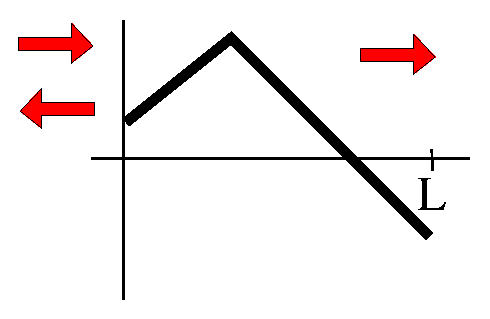
\includegraphics{pictures/transmission_derivation_14_LR}}
\scalebox{0.5}{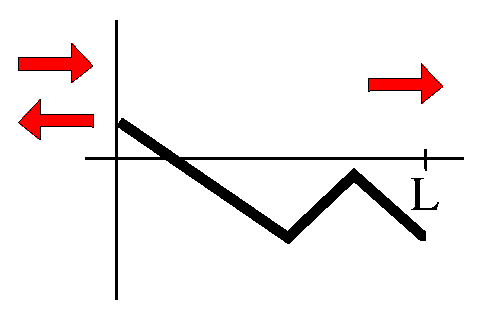
\includegraphics{pictures/transmission_derivation_34_LR}}
\scalebox{0.5}{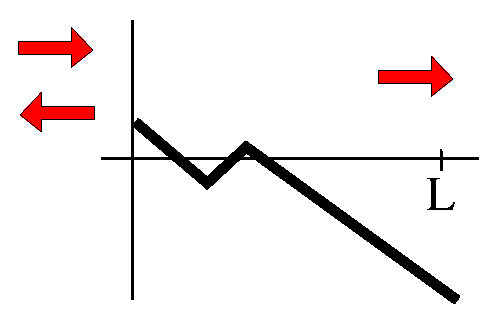
\includegraphics{pictures/transmission_derivation_off_res_LR}}
}
\vskip -0.5cm
\caption{Log of energy versus position sketches for a center of localization in the first half (left), Eq.~\ref{fig:left}; and second half (center), Eq.~\ref{fig:right}. The turning point in the center plot is $L-2 x_o$. The right sketch is off-resonance but prior to pure exponential decay, which applies to any center of localization position, as described by Eq.~\ref{fig:startingequations}. The turning point in the right plot from the initial exponential decay to growth varies depending how far off resonance one is. We call this $x_1$}
\label{fig:cononicaldefectpositions}
\end{figure}
\end{comment}

From the off-resonance Eq.~\ref{fig:startingequations}, we apply boundry conditions to determine the coefficients in passive systems. We take gain into account and make corrections later.

At $x=0$ then $y_1=4$, giving $A=4$. Thus
\begin{equation}
\boxed{y_1 = 4 \exp\left(-\frac{2 x}{\xi}\right)}   \quad \quad \quad 0 < x < L-2 x_o 
\end{equation}

At $x=L$, $y_3=T$. Solve for C,
\begin{equation}
C=T \exp\left(\frac{2(L-x_o)}{\xi}\right)
\end{equation}
plug back in,
\begin{equation}
y_3 = T \exp\left(\frac{2(L-x_o)}{\xi}) \exp(-\frac{2 (x-x_o)}{\xi}\right)  \quad \quad \quad  x_o < x < L
\end{equation}
simplify to get
\begin{equation}
\boxed{y_3 = T \exp\left(-\frac{2(x-L)}{\xi}\right)}  \quad \quad \quad  x_o < x < L
\end{equation}
at $x_o$, $y_2 = y_3$
\begin{equation}
B \exp\left(\frac{2 (x_o-x_o)}{\xi}\right) = B = T \exp\left(-\frac{2(x_o-L)}{\xi}\right)
\end{equation}
plug in to $y_2$
\begin{equation}
y_2 = T \exp\left(-\frac{2(x_o-L)}{\xi}\right) \exp\left(\frac{2 (x-x_o)}{\xi}\right) \quad \quad \quad L-2 x_o < x < x_o 
\end{equation}
simplify to get
\begin{equation}
\boxed{y_2 = T \exp\left(\frac{2(x+L-2 x_o)}{\xi}\right)} \quad \quad \quad L-2 x_o < x < x_o 
\end{equation}

The turning point $x_1$ varies as a function of frequency. Boundry conditions on $x_1$ are that it should remain less than $x_o$ and that it be non-negative. To solve for $x_1$, see where $y_1=y_2$
\begin{equation}
4 \exp\left(-\frac{2 x_1}{\xi}\right) = T \exp\left(\frac{2(x_1+L-2 x_o)}{\xi}\right)
\end{equation}

\begin{equation}
\boxed{x_1(\omega) = -\frac{\xi}{4} \log(\frac{1}{4} T) - \frac{1}{2}L + x_o}
\end{equation}

Knowing $y_1,y_2$, and $y_3$ we can integrate to find the energy ${\cal E}$:
\begin{equation}
\begin{gathered}
{\cal E}(x,\omega) = \int _0 ^{x_1} 4 \exp\left(-\frac{2 x}{\xi}\right) dx +
    \int _{x_1} ^{x_o} T \exp\left(\frac{2(x+L-2 x_o)}{\xi}\right) dx + \\
    \int _{x_o} ^{L} T \exp\left(-\frac{2(x-L)}{\xi}\right)
\label{fig:Eintegral}
\end{gathered}
\end{equation}

Solve, reduce to get the energy as a function of x, frequency, and transmission:
\begin{equation}
\begin{gathered}
{\cal E}(x,\omega) = \frac{\xi}{2} \left( T \left( \exp\left(\frac{2(L-x_o)}{\xi}\right) - \exp\left(\frac{2(L-2 x_o+x_1)}{\xi}\right)+\right. \right.\\
\left.\left.\exp\left(\frac{2(L-x_o))}{\xi}\right) -1 \right) + 4 \left(1-\exp\left(-\frac{2 x_1}{\xi}\right)\right) \right)
\label{fig:appendixenergy}
\end{gathered}
\end{equation}



\specialhead{BIBLIOGRAPHY}
\remline
%\singlespace
\bibliography{../../research/Bibliography/latex_bibliography}
% for an example, see http://amath.colorado.edu/documentation/LaTeX/reference/faq/bibstyles.html
%%20091214%%\bibliographystyle{abbrv}  % numbered alphabetical list
\bibliographystyle{unsrt} % in order to citation. Problem: forces lower case 
%\bibliographystyle{unsrtnat} % NOT what I want

%%20091214%%\addcontentsline{toc}{chapter}{Curriculum Vitae}
%%20091214%%%\specialhead{VITA}

Ben Payne was born on the planet Earth. As a Boy Scout he achieved the rank of Eagle Scout. From 2001 to 2008 he served as a crew chief on F-16s in the Air National Guard, earning an Associates degree in Aircraft Maintenance Technology from the Community College of the Air Force. At the University of Wisconsin-Madison he served as President and then Secretary of the UW-Madison Physics club from 2005 to 2007. He earned a Bachelors of Science from UW-Madison, majoring in both ``Applied Math, Engineering, and Physics'' and also in Physics. During this time he earned his private pilots license and skydiving license. While an undergraduate in Madison, Ben worked as a Network Administrator at the UW-Madison Office of the Registrar from 2002 to 2007. 

After he moved to Missouri, Ben was the founding employee at Micom LLC, again working as a Network Administrator. At Missouri University of Science and Technology he earned his Masters of Science in 2009 and Doctorate of Philosophy in May 2012. While there he greatly enjoyed his work as a research assistant to Dr. Alexey Yamilov for five years. He served as a teaching assistant in a unique role, helping to rewrite the undergraduate course content. In addition to publishing the papers presented in this dissertation, Ben presented his research at scientific meetings and participated in conferences discussing challenges in high performance computing. This was possible as a result of his securing competitive funding from the National Science Foundation. Ben earned multiple competition prizes for presentations given at the Missouri S\&T Physics department. He won awards from the Council of Graduate Students for ``Best Representative'' for two consecutive years. While in Rolla he served as the primary officer of the Missouri S\&T Skydiving club from~2007 to~2012. 


\newpage 
\printglossary
% make sure the glossary shows up in table of contents:
\addcontentsline{toc}{chapter}{Glossary}

\newpage
\printindex
\addcontentsline{toc}{chapter}{Index}

\end{document}
